\documentclass[12pt,oneside]{uhthesis}
% \usepackage{subfigure}
\usepackage[ruled,lined,linesnumbered,titlenumbered,algochapter,spanish,onelanguage]{algorithm2e}
\usepackage{amsmath}
\usepackage{amssymb}
\usepackage{amsbsy}
\usepackage{caption,booktabs}
\usepackage{subcaption}
\captionsetup{ justification = centering }
%\usepackage{mathpazo}
\usepackage{float}
\setlength{\marginparwidth}{2cm}
\usepackage{todonotes}
\usepackage{listings}
\usepackage{xcolor}
\usepackage{hyperref}
\usepackage[utf8]{inputenc}
\usepackage{enumitem}
\usepackage{diagbox}
\usepackage{multirow}
\usepackage{multicol}
\usepackage{textcomp}
\usepackage{graphicx}
\usepackage{tikz}
\usepackage{pgfplots}
\pgfplotsset{compat=1.18}
\usepgfplotslibrary{statistics}
\usepackage{adjustbox}
\usepackage{mdframed}
\usepackage{makecell}
\usepackage{longtable}
\usepackage[spanish]{babel}
% \hypersetup{
%     colorlinks=true,   % Activa el color en los textos con enlaces
%     linkcolor=blue,    % El glosario, ecuaciones e índices se verán azules
%     citecolor=black,   % Las citas bibliográficas se quedan en negro (opcional)
%     urlcolor=blue      % Los enlaces a páginas web externas serán azules
% }
\usepackage[acronym]{glossaries}
\makeglossaries
\definecolor{mygrey}{rgb}{0.95,0.95,0.95} % Un gris claro para el fondo
\mdfsetup{
    backgroundcolor=mygrey,
    linewidth=0pt, % Sin borde
    innertopmargin=1em, % Margen interno superior
    innerbottommargin=1em, % Margen interno inferior
    innerleftmargin=1.5em, % Margen interno izquierdo (para simular indentación)
    innerrightmargin=1.5em % Margen interno derecho
}
\floatstyle{plaintop}
\restylefloat{table}
\addbibresource{Bibliography.bib}
% \setlength{\parskip}{\baselineskip}%
\renewcommand{\tablename}{Tabla}
\renewcommand{\listalgorithmcfname}{Índice de Algoritmos}
%\dontprintsemicolon
\SetAlgoNoEnd

\definecolor{codegreen}{rgb}{0,0.6,0}
\definecolor{codegray}{rgb}{0.5,0.5,0.5}
\definecolor{codepurple}{rgb}{0.58,0,0.82}
\definecolor{backcolour}{rgb}{0.95,0.95,0.92}

% Lenguaje TypeScript
\lstdefinelanguage{TypeScript}{
    keywords={break, case, catch, continue, debugger, default, delete, do, else, finally, for, function, if, in, instanceof, new, return, switch, this, throw, try, typeof, var, void, while, with, class, const, enum, export, extends, import, let, private, public, static, super, interface, implements, async, await, from, as, any, boolean, string, number},
    keywordstyle=\color{purple}\bfseries,
    sensitive=true,
    morecomment=[l]{//},
    morecomment=[s]{/*}{*/},
    morestring=[b]',
    morestring=[b]",
}

% Lenguaje Dockerfile
\lstdefinelanguage{Dockerfile}{
    keywords={FROM, RUN, COPY, WORKDIR, EXPOSE, ENV, ENTRYPOINT, CMD, AS},
    keywordstyle=\color{blue}\bfseries,
    sensitive=true,
    morecomment=[l]{\#},
    morestring=[b]",
    morestring=[b]',
}

% Lenguaje JSON
\lstdefinelanguage{JSON}{
    keywords={true, false, null},
    keywordstyle=\color{purple}\bfseries,
    sensitive=true,
    morestring=[b]",
    morestring=[b]',
    literate={{{$}{$\{$}}1 {{}$}{$\}$}}1
}


\lstdefinestyle{mystyle}{
    backgroundcolor=\color{backcolour},   
    commentstyle=\color{codegreen},
    keywordstyle=\color{purple},
    numberstyle=\tiny\color{codegray},
    stringstyle=\color{codepurple},
    basicstyle=\ttfamily\footnotesize,
    breakatwhitespace=false,         
    breaklines=true,                 
    captionpos=b,                    
    keepspaces=true,                 
    numbers=left,                    
    numbersep=5pt,                  
    showspaces=false,                
    showstringspaces=false,
    showtabs=false,                  
    tabsize=4
}

% \lstdefinelanguage{JavaScript}{
%     keywords={import, export, const, from, function, return, let, new, if, else, for, typeof, var, true, false, null, undefined},
%     keywordstyle=\color{blue}\bfseries,
%     sensitive=true,
%     comment=[l]{//},
%     morecomment=[s]{/*}{*/},
%     commentstyle=\color{gray}\itshape,
%     stringstyle=\color{red},
%     morestring=[b]',
%     morestring=[b]",
%     basicstyle=\ttfamily\footnotesize,
%     breaklines=true,
%     frame=single,
%     numbers=left,
%     numbersep=5pt,
%     showstringspaces=false,
% }

% \lstset{
%     basicstyle=\ttfamily\small\color{white},
%     breaklines=true,
%     frame=none,
%     numbers=left,
%     numberstyle=\tiny\color{gray},
%     tabsize=4,
%     showstringspaces=false,
%     backgroundcolor=\color{darkgray},
%     inputencoding=utf8,
%     extendedchars=true,
%     literate={á}{{\'a}}1 {é}{{\'e}}1 {í}{{\'i}}1 {ó}{{\'o}}1 {ú}{{\'u}}1
%              {Á}{{\'A}}1 {É}{{\'E}}1 {Í}{{\'I}}1 {Ó}{{\'O}}1 {Ú}{{\'U}}1
%              {ñ}{{\~n}}1 {Ñ}{{\~N}}1
% }


\lstset{style=mystyle}


\title{Sistema web para el autorreporte de Eventos Supuestamente Atribuibles a la Vacunación o Inmunización (ESAVI) en el Instituto Finlay de Vacunas (IFV)}
\author{\\\vspace{0.25cm}Jabel Resendiz Aguirre}
\advisor{\\\vspace{0.25cm}MsC. Joanna Campbell Amos\\\vspace{0.2cm}MsC. Aracelys García Armenteros}
\degree{Licenciado en Ciencia de la Computación}
\faculty{Facultad de Matemática y Computación}
\date{\today \\\vspace{0.25cm}\href{https://github.com/JabelResendiz/thesis}{github.com/JabelResendiz/thesis}}
\logo{Graphics/uhlogo}
\makenomenclature

\renewcommand{\vec}[1]{\boldsymbol{#1}}
\newcommand{\diff}[1]{\ensuremath{\mathrm{d}#1}}
\newcommand{\me}[1]{\mathrm{e}^{#1}}
\newcommand{\pf}{\mathfrak{p}}
\newcommand{\qf}{\mathfrak{q}}
%\newcommand{\kf}{\mathfrak{k}}
\newcommand{\kt}{\mathtt{k}}
\newcommand{\mf}{\mathfrak{m}}
\newcommand{\hf}{\mathfrak{h}}
\newcommand{\fac}{\mathrm{fac}}
\newcommand{\maxx}[1]{\max\left\{ #1 \right\} }
\newcommand{\minn}[1]{\min\left\{ #1 \right\} }
\newcommand{\lldpcf}{1.25}
\newcommand{\nnorm}[1]{\left\lvert #1 \right\rvert }
\renewcommand{\lstlistingname}{Ejemplo de código}
\renewcommand{\lstlistlistingname}{Ejemplos de código}

\begin{document}

\frontmatter
\maketitle

%  \begin{dedication}
    A mi familia, a mis profesores, a mis amigos y compañeros de la carrera, \\
    por sostenerme cuando el código no compilaba y la vida tampoco.
\end{dedication}
%  \begin{acknowledgements}
    Agradecemos al Proyecto PN223LH010-042 "Nuevas aproximaciones en la modelación dinámica de enfermedades", del Programa Nacional de Ciencias Básicas 2024-2026, y a la Unidad Docente-Investigativa IFV\_MATCOM por su invaluable apoyo.
\end{acknowledgements}
%  \begin{opinion}

    \noindent\textbf{Título:} Sistema web para el autorreporte de Eventos Supuestamente Atribuibles a la Vacunación o Inmunización (ESAVI) en el Instituto Finlay de Vacunas (IFV)\\
    \textbf{Autor:} Jabel Resendiz Aguirre\\
    \textbf{Tutores:} MSc. Joanna Campbell Amos, MSc. Aracelys García Armenteros, Lic. Javier Rodríguez Sánchez
    
    \vspace{0.5cm}
    
    Los que suscribimos, tutores del trabajo de diploma de Jabel Resendiz Aguirre, queremos expresar desde el inicio nuestra profunda satisfacción con el resultado alcanzado. El tema abordado —un sistema web para el autorreporte de eventos adversos en farmacovigilancia— exigía no solo dominio técnico, sino también una sensibilidad especial para comprender un problema de salud pública. Jabel demostró madurez intelectual y compromiso desde la primera reunión, asumiendo con responsabilidad cada sugerencia y devolviéndonos siempre más de lo que pedíamos. Esa chispa de superación constante ha sido, sin dudas, el sello distintivo de su proceso formativo.
    
    A lo largo de los capítulos 1 y 2, Jabel realizó una exhaustiva revisión del estado del arte sobre sistemas de farmacovigilancia, normas internacionales y tecnologías web para el manejo de datos sensibles. Lo que más nos impresionó fue su capacidad para aprender de manera autodidacta: frameworks front-end, protocolos de seguridad y validación de formularios médicos eran territorios nuevos para él, pero los conquistó con perseverancia y método. 
    
    En el capítulo 3, propone e implementa una solución funcional, escalable y centrada en el usuario, donde la usabilidad y la confidencialidad se integran con buen criterio. Cada línea de código y cada decisión arquitectónica reflejan horas de trabajo silencioso, pero también de consultas activas a sus tutores, demostrando que sabe equilibrar la independencia con la búsqueda oportuna de orientación.
    
    Por todo ello, como tutores nos sentimos orgullosos del camino recorrido junto a Jabel. Consideramos que su tesis cumple holgadamente los requisitos académicos de una licenciatura y aporta una herramienta con potencial real para el sistema de salud. Es un alumno que no solo aprende, sino que también sabe escuchar, preguntar y agradecer —cualidades que enriquecen cualquier vínculo educativo. Por todo lo anterior, proponemos al tribunal que se le otorgue la calificación de \textbf{Excelente (5)}.
    
    \vspace{1.5cm}
    
    \begin{flushright}
        La Habana, junio de 2026
    \end{flushright}
    
    \vspace{3cm}
    
    \begin{flushright}
        \begin{minipage}{0.3\textwidth}
            \centering
            
\includegraphics[width=4.5cm, height=2.5cm, keepaspectratio]{Graphics/firma_joanna.png}\\[0.2cm]
            \rule{4.5cm}{0.4pt}\\[0.1cm]
            \small MSc. Joanna Campbell Amos
        \end{minipage}%
        \hfill
        \begin{minipage}{0.3\textwidth}
            \centering
            
\includegraphics[width=4.5cm, height=2.5cm, keepaspectratio]{Graphics/firma_aracelys.png}\\[0.2cm]
            \rule{4.5cm}{0.4pt}\\[0.1cm]
            \small MSc. Aracelys García Armenteros
        \end{minipage}%
        \hfill
        \begin{minipage}{0.3\textwidth}
            \centering
            
\includegraphics[width=4.5cm, height=2.5cm, keepaspectratio]{Graphics/firma_javier.png}\\[0.2cm]
            \rule{4.5cm}{0.4pt}\\[0.1cm]
            \small Lic. Javier Rodríguez Sánchez
        \end{minipage}
    \end{flushright}
    

\end{opinion}
  \begin{resumen}
	La implementación del sistema web para la gestión de ESAVI se fundamenta en una arquitectura modular basada en los principios de Clean Architecture, utilizando .NET 8 para el backend y React con TypeScript para el frontend. 
	La solución integra mecanismos avanzados de seguridad, incluyendo autenticación mediante JWT con rotación de refresh tokens almacenados en cookies HttpOnly, limitación de velocidad (rate limiting) y protección contra ataques automatizados mediante Friendly CAPTCHA. 
	Para optimizar la experiencia del usuario y la fiabilidad, se implementó una comunicación asíncrona empleando RabbitMQ y MassTransit, facilitando notificaciones automáticas vía correo electrónico y WhatsApp. 
	El sistema garantiza la integridad y trazabilidad de los datos de farmacovigilancia mediante el uso del patrón Unit of Work y un registro de auditoría automatizado sobre una base de datos MySQL.
\end{resumen}

\begin{abstract}
	The implementation of the ESAVI management web system is based on a modular architecture following Clean Architecture principles. 
	The backend was developed using .NET 8 and C\#, while the frontend was built as a Single Page Application (SPA) with React and TypeScript. 
	The system features a robust security framework, including JWT authentication with Refresh Token rotation (HttpOnly cookies), IP-based rate limiting, and Friendly CAPTCHA protection for public endpoints. 
	To ensure high availability and responsiveness, the solution incorporates asynchronous messaging via RabbitMQ and MassTransit for automated email and WhatsApp notifications. 
	Data integrity and traceability are managed through Entity Framework Core, the Unit of Work pattern, and an automated Audit Log system.
\end{abstract}
%  \include{FrontMatter/Contents}

\mainmatter

% \chapter{Introducción}\label{chapter:introduction}
\addcontentsline{toc}{chapter}{Introducción}

La medicina moderna ha fortalecido el control de enfermedades mediante el desarrollo de vacunas. 
Sin embargo, su aplicación masiva en la población exige garantizar su seguridad de manera rigurosa y continua.
Esta exigencia toma forma en un proceso escalonado de investigación clínica, que transcurre por diversas etapas antes de la aprobación del fármaco, tal como ilustra la figura \ref{fig:desarrollo_clinico}.

En las etapas I, II y III, el producto atraviesa estudios controlados en grupos seleccionados de voluntarios para reunir datos preliminares sobre su seguridad y definir las recomendaciones de posología y eficacia a corto plazo. 
Durante estas fases, el producto biológico permanece en un entorno científico resguardado, donde la población de estudio es reducida (rara vez superando los 5,000 sujetos) y generalmente homogénea, lo que limita la detección de reacciones poco frecuentes \cite{who_pharmacovigilance_2004}.

\begin{figure}[htbp]
    \centering
    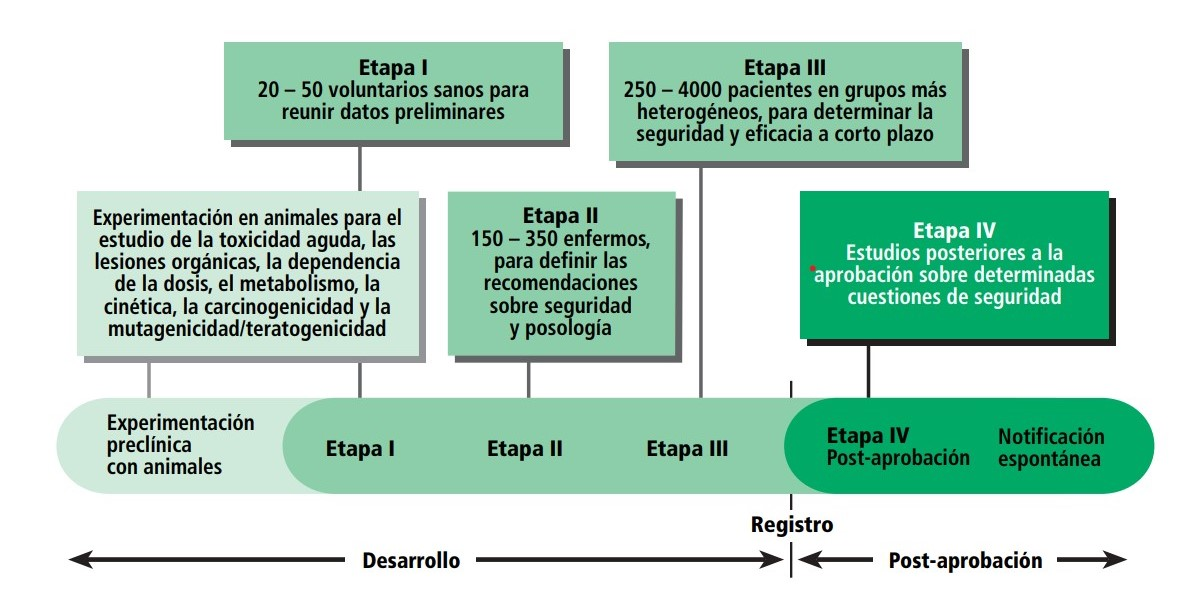
\includegraphics[width=0.8\textwidth]{Graphics/Cap1/fig1_desarrollo_clinico.jpg}
    \caption{Etapas del desarrollo clínico de vacunas. Adaptado de \cite{who_pharmacovigilance_2004}.}
    \label{fig:desarrollo_clinico}
\end{figure}

Una vez que la \gls{vacuna} recibe el registro sanitario y comienza su uso masivo en la población general, inicia la etapa IV o post-aprobación. 
En estas condiciones reales de uso, el escenario cambia drásticamente: el producto alcanza a grupos diversos que incluyen niños, ancianos, embarazadas y personas con múltiples patologías, quienes a menudo fueron excluidos de los ensayos iniciales \cite{who_pharmacovigilance_2004}.

Precisamente en esta fase es donde comienzan a manifestarse los eventos supuestamente atribuibles a la vacunación o inmunización (ESAVI), definidos como cualquier cuadro clínico desfavorable (signo, síntoma o enfermedad) que ocurre tras la vacunación y no necesariamente tiene una relación causal con la vacuna \cite{paho_curso_esavi}.

Para gestionar estos riesgos inevitables, surge la \gls{farmacovigilancia} como la ciencia y las actividades relativas a la detección, evaluación, comprensión y prevención de los efectos adversos de los medicamentos.
Esta disciplina permite evaluar continuamente la relación beneficio-riesgo y detectar señales de alerta que no fueron identificadas durante las fases iniciales de investigación \cite{who_pharmacovigilance_2004}.

\section{Contexto histórico y social de la farmacovigilancia}\label{section:contextoHistoricoSocial}

La evolución de la farmacovigilancia ha estado marcada por tragedias sanitarias —como el desastre de la talidomida en 1961— que evidenciaron la necesidad de sistemas formales de vigilancia\cite{tarrago_farmacovigilancia_cuba_2019,palacios2021talidomida}. 
Como respuesta, la Organización Mundial de la Salud (\gls{oms}) impulsó mecanismos internacionales que dieron origen al Centro de Monitoreo de Uppsala \cite{barrero2022notificacion}. 
Desde los primeros intentos de notificación voluntaria y el modelo de la Tarjeta Amarilla (ver glosario \gls{tarjeta_amarilla}) en papel, la práctica ha transitado hacia repositorios globales como VigiBase (ver glosario \gls{VigiBase}), que centraliza más de 20 millones de registros y exige la automatización para procesar flujos masivos de datos.

\subsection{La farmacovigilancia en Cuba}

El país posee una sólida trayectoria en seguridad de medicamentos. 
Cuba ingresó al Programa Internacional de Monitoreo de Medicamentos de la \gls{oms} en 1994 y consolidó su Sistema Cubano de Farmacovigilancia (\gls{scfv}) en 1999 \cite{tarrago_farmacovigilancia_cuba_2019, paho_vigilancia_medicamentos_cuba}.

Los indicadores del sistema cubano superan los estándares internacionales. Mientras la tasa eficiente global oscila entre 250 y 300 notificaciones por millón de habitantes al año, el país alcanzó en 2020 un total de 13,025 reportes, lo que representa una tasa de 1,163 por millón de habitantes \cite{cecmed_farmacovigilancia_cuba_2020} (véase Anexo \ref{app:reportes_cuba_2020}). 
Sin embargo, al analizar la distribución por grupo farmacológico, la mayoría de los reportes corresponde a medicamentos de uso frecuente, mientras que los eventos asociados a vacunas representan una proporción menor, con alrededor de 700 reportes (véase Anexo \ref{app:grupo_farmacologico}).

La nación alcanzó un desempeño destacado, situándose entre los 20 países con mayores tasas de notificación a nivel mundial \cite{normas_farmacovigilancia_cuba_2012}. En el ámbito específico de las vacunas, mediante su sistema de vigilancia de los \glspl{esavi}, ocupó en 2018 el tercer lugar en la región de las Américas, con 6,682 reportes, solo detrás de Estados Unidos y Brasil \cite{ops_manual_esavi_2021}. La figura \ref{fig:esavi_paises_americas} (véase Anexo \ref{app:esavi_por_paises}) ilustra este comportamiento.

Detrás de estos indicadores existe una estructura organizativa consolidada. 
El sistema de vigilancia de medicamentos opera bajo la rectoría del \gls{cecmed}, con una red coordinada que integra a la \gls{ucnfv}, los fabricantes (QUIMEFA), las redes de distribución mayorista y minorista, el \gls{cenatox} y la vigilancia especializada de vacunas a cargo del \gls{pai} \cite{paho_vigilancia_medicamentos_cuba}. 
Cada uno de estos actores tiene la obligación de informar sobre los problemas detectados en sus respectivos ámbitos (calidad, seguridad, distribución, toxicidad, vacunas) a través de los canales establecidos.
Toda la información fluye hacia el Observatorio de Vigilancia Postcomercialización del \gls{cecmed}, encargado de evaluar la relación beneficio-riesgo para emitir alertas o retirar lotes.

\subsection{Instituto Finlay de Vacunas: contexto y rol como fabricante nacional}

El Instituto Finlay de Vacunas (\gls{ifv}) es una organización científica y empresa estatal de alta tecnología cubana, integrada al Grupo de las Industrias Biotecnológica y Farmacéutica de Cuba ,\gls{biocubafarma}, que opera bajo un modelo de ciclo cerrado que abarca desde la investigación básica hasta la comercialización y el seguimiento postcomercialización \cite{finlay_instituto_2026}.

Como pilar estratégico de la soberanía tecnológica del país, el instituto garantiza la producción de 8 de las 11 vacunas administradas por el Programa Nacional de Inmunización, proveyendo el 78\% de las dosis totales del sistema de salud \cite{carbonell_cmi_finlay_2016}.

Su trayectoria de innovación incluye hitos científicos mundiales como la VA-MENGOC-BC® —primera vacuna eficaz contra el serogrupo B de la meningitis— y la Quimi-Hib, la primera vacuna conjugada con un antígeno totalmente sintético. 
Durante la crisis sanitaria global, el \gls{ifv} reafirmó su liderazgo al desarrollar la línea de vacunas SOBERANA contra la COVID-19, logrando una escala de operación sin precedentes con más de 38,7 millones de dosis administradas al cierre de julio de 2022 \cite{finlay_instituto_2026}. 
Internacionalmente, su prestigio descansa en exportaciones y colaboraciones estratégicas que impactan en más de 17 países de América Latina, Asia y África \cite{carbonell_cmi_finlay_2016}.



\section{Antecedentes, Motivación y Justificación}\label{section:antecedentesMotivacionJustificacion}

El sistema cubano de farmacovigilancia estructura el reporte de eventos adversos en tres niveles: municipal (profesionales o pacientes llenan formularios en papel como los modelos 33-36-02 y 84-30-2), provincial (16 unidades coordinan y validan los reportes) y nacional (la \gls{ucnfv} administra la base \gls{FarmaVigiC} con 75 variables clínicas). 
Los casos graves exigen notificación en menos de 24 horas, mientras que el flujo regular es quincenal \cite{tarrago_farmacovigilancia_cuba_2019,normas_farmacovigilancia_cuba_2012}. 
A nivel internacional, los datos validados viajan trimestralmente a \gls{VigiBase} mediante los estándares \gls{WHO-ART} e \gls{ICD-10} \cite{normas_farmacovigilancia_cuba_2012} (véanse Anexos \ref{app:modelos_formularios}).

Sin embargo, este modelo presenta deficiencias que afectan su operatividad. 
La dependencia de formularios en papel y su transcripción manual reducen la notificación a apenas entre el 5\% y el 10\% de las reacciones adversas que realmente ocurren en la población, fenómeno conocido como \gls{infranotificacion} \cite{tarrago_farmacovigilancia_cuba_2019}.
Adicionalmente, tanto la base nacional \gls{FarmaVigiC} como el propio \gls{ifv} sustentan su gestión de datos en hojas de cálculo (Excel), un formato rudimentario que limita la integridad y escalabilidad del procesamiento \cite{normas_farmacovigilancia_cuba_2012}.


De forma transversal, los fabricantes como el \gls{ifv} participan mediante un flujo bidireccional con la autoridad reguladora. 
A través de convenios con la \gls{ucnfv}, tienen acceso a la base nacional y reciben retroalimentación sobre la seguridad de sus productos, a la vez que están obligados a notificar sus \gls{ips} (ver glosario \gls{ips}) \cite{normas_farmacovigilancia_cuba_2012}.
Por su parte, la autoridad nacional les transmite alertas de forma ágil —especialmente en casos graves o mortales— y comparte señales de riesgo identificadas, permitiendo a los fabricantes actualizar la información de seguridad de sus productos y aplicar estrategias de minimización de riesgos \cite{normas_farmacovigilancia_cuba_2012}.
El ciclo quincenal de actualización introduce una latencia de 15 días, lo que retrasa la detección de señales de seguridad y afecta la elaboración oportuna de los \gls{ips} por parte de los fabricantes \cite{normas_farmacovigilancia_cuba_2012}.

No obstante, el propio IFV carece de una base de datos formal y digitalizada que le permita capturar y procesar de forma inmediata los reportes vinculados a sus vacunas.




\section{Presentación del problema científico}\label{section:presentacionProblema}

A pesar de su alto nivel tecnológico, el \gls{ifv} presenta una brecha en la gestión digital de los datos de seguridad postcomercialización, aún dependiente de procesos manuales. 

Desde una perspectiva computacional, esta situación comprende las siguientes limitaciones internas, cuantificadas a partir de los indicadores históricos del sistema cubano de farmacovigilancia:

\begin{enumerate}[label=L\arabic*]
\item \textbf{Fragmentación de la infraestructura de datos:} El IFV gestiona la información de seguridad de sus vacunas mediante herramientas no estandarizadas (hojas de cálculo, archivos sueltos), sin contar con una base de datos formal. El estado deseado implica un modelo de datos que garantice un procesamiento ágil y estructurado.

\item \textbf{Retrasos en el procesamiento y análisis de la información:} El flujo actual de notificación de los \glspl{esavi} descansa en un ciclo quincenal, lo que introduce una demora de 15 días entre la ocurrencia del evento y su disponibilidad para el análisis por parte del \gls{ifv}. 
Frente a ello, el instituto necesita una solución que permita la notificación inmediata, especialmente para eventos graves.

\item \textbf{Barreras en la captura ciudadana:} La dependencia de formularios en papel y la ausencia de canales digitales directos generan una tasa de infranotificación estimada entre el 90\% y el 95\%. 
El instituto necesita un canal digital de autorreporte accesible al ciudadano y profesionales de la salud.

\item \textbf{Aislamiento del ciudadano en el seguimiento de su reporte:} El sistema actual no proporciona al paciente o ciudadano ningún canal ágil para conocer el estado de su reporte una vez entregado. 
Esta falta de retroalimentación genera desconfianza en el proceso de farmacovigilancia, desmotiva futuras notificaciones y contribuye a la percepción de que el reporte ``no sirve para nada'' o ``termina extraviado en el sistema''. 
El estado deseado incluye un mecanismo de trazabilidad que permita al ciudadano consultar el estado de su reporte en todo momento.
 
\end{enumerate}


A partir de las limitaciones identificadas, el problema científico queda definido como:

\textit{La combinación de fragmentación de datos, latencia de 15 días, infranotificación >90\% y aislamiento del ciudadano impide una gestión oportuna, íntegra y confiable de los eventos supuestamente atribuibles a la vacunación o inmunización (ESAVI) en el IFV.}

De este problema surge la siguiente pregunta científica:

¿Cómo reducir la infranotificación y latencia en la gestión de eventos supuestamente atribuibles a la vacunación o inmunización (ESAVI) en el \gls{ifv} mediante un sistema de autorreporte web que integre validación estructurada de datos?

\section{Objetivo general y objetivos específicos}\label{section:objetivosPrincipalesEspecificos}

El objetivo general de la presente investigación consiste en desarrollar un sistema informático, en forma de aplicación web, que permita la notificación ciudadana, el almacenamiento estructurado y la consulta de los \glspl{esavi} con trazabilidad en el contexto de la farmacovigilancia del Instituto Finlay de Vacunas.

De este objetivo general surgen los siguientes objetivos específicos:

\begin{enumerate}
    \item \textbf{Investigar el estado del arte} de sistemas de farmacovigilancia, analizando comparativamente al menos tres sistemas (VAERS, NotificaRAM y V-Safe) en términos de sus modelos de datos, flujos de notificación, mecanismos de interoperabilidad y estrategias de privacidad.
    
    \item \textbf{Diseñar un modelo de datos relacional} que estructure las variables clínicas esenciales para la captura y gestión de los ESAVI en el instituto, garantizando la integridad referencial y la compatibilidad de exportación hacia los formatos requeridos por la entidad regulatoria.
    
    \item \textbf{Definir la arquitectura del sistema} basada en principios de diseño modular e independencia de la infraestructura (arquitectura limpia), que garantice la escalabilidad y la facilidad de mantenimiento del sistema.
    
    \item \textbf{Implementar un Mínimo Producto Viable (MVP)} que integre la captura ciudadana de eventos adversos, la gestión de revisiones médicas por niveles de acceso y mecanismos de seguridad informática para la protección de datos sensibles.
    
    \item \textbf{Validar el funcionamiento del sistema} mediante una evaluación integral que verifique el cumplimiento de los requerimientos funcionales, el comportamiento bajo carga concurrente, la calidad del despliegue web y la usabilidad percibida por los usuarios finales.
    
\end{enumerate}



\section{Actualidad, Novedad e Importancia}\label{section:actualidadNovedadImportancia}


\subsection{Actualidad}


La actualidad de esta investigación responde a la imperativa transición del IFV hacia infraestructuras digitales soberanas, capaces de procesar flujos masivos de datos en tiempo real tras el éxito de la serie SOBERANA. 
En un contexto global donde la farmacovigilancia exige la automatización y el empoderamiento del paciente a través del autorreporte digital.
Resulta crítico alinear la gestión institucional con los actuales enfoques de eficiencia empresarial en Cuba, priorizando la toma de decisiones basada en evidencia clínica inmediata frente a los modelos manuales tradicionales.

\subsection{Novedad Científica}

La novedad de este trabajo reside en el diseño e implementación de un sistema web centralizado, diseñado específicamente para que el fabricante gestione de forma soberana la seguridad de sus vacunas. A diferencia de los métodos actuales basados en registros manuales y hojas de cálculo, esta solución aporta los siguientes elementos innovadores desde una perspectiva computacional:

\begin{enumerate}
    \item \textbf{Arquitectura de \gls{autorreporte} con validación en origen:} El sistema captura el dato en la fuente mediante validaciones sintácticas y semánticas en tiempo real, garantizando la integridad y consistencia clínica desde el momento del registro por parte de médicos o pacientes.
    
    \item \textbf{Automatización de alertas por eventos graves:} Un motor de reglas de negocio detecta automáticamente casos graves (p. ej., muerte, hospitalización) y dispara notificaciones al equipo de farmacovigilancia del \gls{ifv}, eliminando el retardo quincenal del sistema actual.
    
    \item \textbf{Industrialización del análisis:} El sistema sustituye los procesos manuales de consolidación por cuadros de mando (dashboards) dinámicos, que actualizan indicadores de riesgo en tiempo real a partir de los reportes almacenados.
    
    \item \textbf{Mensajería asíncrona para notificaciones:} El sistema incorpora una cola de mensajes basada en RabbitMQ que desacopla la generación de reportes del envío de notificaciones por correo electrónico, garantizando la entrega confiable y no bloqueante.
    
    \item \textbf{Seguimiento y trazabilidad del reporte:} El sistema permite al usuario (paciente o médico) consultar en cualquier momento el estado de su reporte (recibido, en validación, procesado, cerrado), proporcionando transparencia y confianza en el proceso.
    
    \item \textbf{Mecanismo de seguridad informática anti-spam:} El sistema incorpora herramientas de protección para prevenir el envío masivo y automatizado de información (\textit{\gls{spam}}),mediante el uso de Friendly CAPTCHA (basado en desafíos criptográficos invisibles) y técnicas de control de frecuencia de solicitudes.
    
\end{enumerate}

Para comprender el alcance de la novedad, la Tabla \ref{tab:comparativa_novedad} contrasta la solución propuesta con el sistema actual en Cuba (FarmaVigiC) y referentes internacionales\footnote{Los referentes internacionales considerados reciben un análisis en el Capítulo \ref{chapter:marco-teorico-referencial} (Sección \ref{subsection:sistemas_autorreporte}).}. 


\begin{table}[ht]
    \centering
    \small
    \caption{Comparativa entre la solución propuesta y los sistemas existentes}
    \label{tab:comparativa_novedad}
    \begin{tabular}{|p{3.8cm}|p{3cm}|p{3cm}|p{3.5cm}|}
        \hline
        \textbf{Característica / Novedad} & \textbf{FarmaVigiC (actual)} & \textbf{Referentes internacionales} & \textbf{Solución propuesta (IFV)} \\
        \hline
        Validación de datos en origen & No (transcripción manual posterior) & Parcial & Sí (validación sintáctica y semántica en tiempo real) \\
        \hline
        Automatización de alertas por eventos graves & No (revisión manual) & Parcial & Sí (motor de reglas, alertas <3 minuto) \\
        \hline
        Industrialización del análisis (dashboards) & No (procesos manuales en Excel) & Parcial & Sí (cuadros de mando dinámicos en tiempo real) \\
        \hline
        Mensajería asíncrona para correos & No aplica & Limitado & Sí (RabbitMQ, entrega confiable y no bloqueante) \\
        \hline
        Seguimiento y trazabilidad del reporte & No (usuario aislado) & Parcial & Sí (consulta de estado: recibido, validación, procesado, cerrado) \\
        \hline
        Seguridad anti-spam & No aplica & Sí (requisito en algunos sistemas) & Sí (CAPTCHA + limitador de velocidad) \\
        \hline
        Canal de autorreporte ciudadano & No (solo profesional sanitario) & Sí (web pública) & Sí (web con validaciones) \\
        \hline
        Tiempo de disponibilidad para fabricante & 15 días (ciclo quincenal) & 24-48 horas & Inmediato (aplicación para fabricante, <3minutos) \\
        \hline
    \end{tabular}
\end{table}


\subsection{Importancia}

La importancia de este trabajo radica en tres dimensiones:

\textbf{Salud pública:} El canal digital de autorreporte elimina barreras físicas y burocráticas, permite capturar datos de forma masiva y favorece la detección temprana de eventos adversos, fortaleciendo la seguridad del paciente y la confianza en los programas de inmunización.

\textbf{Fortalecimiento institucional:} La gestión digital de la información de seguridad permite al Instituto Finlay de Vacunas mejorar su capacidad de análisis y disponer de datos actualizados y trazables para la toma de decisiones sobre sus vacunas.

\textbf{Base para futuras innovaciones:} La estructuración de la información clínica constituye el cimiento para que, en trabajos futuros, el instituto pueda aplicar técnicas de minería de datos o análisis de patrones temporales. El presente trabajo no aborda dichos modelos analíticos, pero sienta las bases técnicas para su implementación posterior.




\section{Estructura del trabajo}\label{section:estructuraTrabajo}

El presente trabajo de investigación consta de cinco capítulos que organizan de manera progresiva los elementos teóricos, metodológicos y prácticos desarrollados:

\begin{itemize}
    \item \textbf{Capítulo 1 - Introducción:} Presenta el diseño teórico de la investigación: el contexto de la farmacovigilancia, la motivación y justificación del estudio en el marco del Instituto Finlay de Vacunas, la formulación del problema científico, y los objetivos que guían el desarrollo del trabajo.

    \item \textbf{Capítulo 2 - Marco Teórico y Referencial:} Aborda el estado del arte relacionado con el objeto de estudio. Analiza sistemas existentes de autorreporte de eventos adversos, así como tecnologías y enfoques de desarrollo, lo que permite fundamentar la selección de las herramientas empleadas en la solución propuesta.

    \item \textbf{Capítulo 3 - Metodología y diseño de la propuesta de solución:} Constituye el núcleo técnico de la investigación. Describe los requerimientos del sistema, los casos de uso, la arquitectura seleccionada y el modelo de datos.

    \item \textbf{Capítulo 4 - Detalles de Implementación:} Expone la materialización concreta del sistema: las tecnologías empleadas, la organización de la solución, los mecanismos de seguridad y la integración entre componentes, así como el despliegue en los entornos definidos.

    \item \textbf{Capítulo 5 - Validación de la aplicación:} Presenta los escenarios de prueba, las herramientas utilizadas y los resultados obtenidos. Evalúa el cumplimiento de los requerimientos definidos y la calidad de la información gestionada por el sistema.

\end{itemize}

Finalmente, el trabajo incluye las conclusiones, que sintetizan los principales aportes de la investigación; las recomendaciones para trabajos futuros y las referencias bibliográficas consultadas.


\section*{Uso de la inteligencia artificial generativa}

% \chapter{Marco Teórico y Referencial}\label{chapter:marco-teorico-referencial}


El presente capítulo establece los fundamentos conceptuales y tecnológicos que sustentan el desarrollo del sistema. El estado del arte revisa las plataformas de farmacovigilancia digital existentes e identifica sus brechas. Los fundamentos de sistemas web y de bases de datos definen la arquitectura y los principios que garantizan la integridad de la información clínica. El capítulo concluye con un análisis comparativo de las tecnologías disponibles para la implementación, cuyos resultados orientan la selección del conjunto de herramientas del sistema.


\section{Marco Referencial (Estado del Arte)}

El marco referencial de este trabajo examina soluciones existentes para la notificación de eventos adversos, desde plataformas genéricas hasta sistemas nacionales de farmacovigilancia, con el fin de identificar sus limitaciones y extraer buenas prácticas que orienten el diseño del sistema ESAVI del IFV.

\subsection{Limitaciones de plataformas genéricas (Google Forms)}

El uso de plataformas de formularios en la nube como Google Forms, Microsoft Forms o JotForm podría considerarse una alternativa rápida para la captura de eventos adversos. Sin embargo, sus características las inhabilitan como solución para un sistema nacional de farmacovigilancia:

\begin{itemize}

\item \textbf{Soberanía de los datos:} La información de salud reside en servidores externos bajo jurisdicciones extranjeras, vulnerando el principio de residencia de datos clínicos que exige el marco regulatorio nacional.

\item \textbf{Validación clínica insuficiente:} Solo ofrecen validaciones básicas (campos obligatorios, formatos). Carecen de capacidad para integrar codificación clínica estandarizada o para implementar reglas de negocio complejas como la coherencia cronológica entre vacunación y aparición de síntomas.

\item \textbf{Ausencia de control de acceso granular:} No permiten definir roles diferenciados (reportante, médico evaluador, jefe de vacunación) con permisos específicos, lo cual es indispensable en un flujo de farmacovigilancia.

\item \textbf{Falta de trazabilidad:} No registran quién modificó un reporte ni cuándo, imposibilitando la auditoría de los datos.

\item \textbf{Interoperabilidad nula:} Los datos requieren exportación manual a hojas de cálculo, impidiendo la integración automatizada con sistemas de información de salud.

\end{itemize}

En consecuencia, estas plataformas son adecuadas para encuestas, pero no para un sistema de autorreporte de ESAVI que requiere seguridad, estructuración, trazabilidad e interoperabilidad. Esta brecha justifica el desarrollo de una solución específica.

\subsection{Análisis de sistemas de autorreporte de eventos adversos existentes}

Los sistemas de autorreporte de eventos adversos operan bajo dos modelos. 
La vigilancia pasiva depende de la iniciativa voluntaria del ciudadano o profesional para notificar un evento. 
La vigilancia activa, en cambio, contacta proactivamente al usuario mediante encuestas digitales para recopilar datos en tiempo casi real.

Este apartado examina cuatro sistemas —VAERS, NotificaRAM, V-safe y el formulario del CECMED— con el objetivo de identificar brechas de diseño que fundamenten la propuesta del sistema ESAVI-IFV.

\subsubsection{Sistema de Notificación de Eventos Adversos a Vacunas (VAERS, por sus siglas en inglés)}

\textbf{VAERS} es el sistema nacional de farmacovigilancia en los Estados Unidos, administrado por la Administración de Alimentos y Medicamentos (FDA, por sus siglas en inglés), agencia reguladora de medicamentos y alimentos, y los Centros para el Control y la Prevención de Enfermedades (CDC, por sus siglas en inglés), organismo responsable del control y prevención de enfermedades \cite{fda_vaers}.
Su objetivo principal es detectar señales de seguridad no identificados durante los ensayos clínicos \cite{cdc_vaers}.

Permite la notificación voluntaria de eventos adversos por parte de profesionales de la salud, fabricantes y ciudadanos mediante formularios web y PDF descargables \cite{vaers_official}.
Para garantizar la integridad del repositorio, la legislación estadounidense contempla sanciones civiles y penales ante el suministro intencional de información falsa en los reportes \cite{vaers_official}. 
Esto contribuye a reducir la introducción de datos malintencionados en un sistema de acceso público.

Los reportes alimentan la base de datos CDC WONDER\footnote{CDC WONDER (Wide-ranging Online Data for Epidemiologic Research): plataforma de los CDC para el acceso público a datos epidemiológicos anonimizados.}, garantizando la transparencia mediante su disponibilidad abierta \cite{vaers_official}. 
Ante una señal de alerta, el monitoreo escala hacia sistemas complementarios de vigilancia activa y evaluación clínica como VSD\footnote{Vaccine Safety Datalink (VSD): red de vigilancia que integra datos de múltiples organizaciones sanitarias para el análisis de seguridad vacunal.} y el proyecto CISA\footnote{Clinical Immunization Safety Assessment (CISA): iniciativa orientada a la evaluación clínica especializada de eventos adversos asociados a la vacunación.} para confirmar posibles riesgos \cite{cdc_vaers}.

El formulario consta de 28 secciones con un nivel de detalle que puede resultar abrumador para un usuario que reporta bajo condiciones de malestar físico. 
Además, información que en el sistema de salud cubano resulta relevante para la evaluación clínica —como síntomas, su intensidad y desenlace— termina resumida en campos de texto libre, lo que genera datos heterogéneos y difíciles de analizar de forma automatizada.


\subsubsection{NotificaRAM}

\textbf{NotificaRAM} es la plataforma oficial de farmacovigilancia en España para la notificación de sospechas de reacciones adversas a medicamentos \cite{aemps_manual_2025}.
\textit{La Agencia Española de Medicamentos y Productos Sanitarios (AEMPS)} gestiona este portal en el marco del Sistema Español de Farmacovigilancia de Medicamentos de Uso Humano (SEFV-H) \cite{aemps_sefv_2025}.

El sistema funciona de forma descentralizada, remitiendo los reportes a los Centros Autonómicos de Farmacovigilancia para su validación técnica inicial \cite{aemps_manual_2025}. 
Tras esta evaluación, la base de datos \textit{FEDRA(Farmacovigilancia Española, Datos de Reacciones Adversas)}, sistema nacional de notificación y almacenamiento de sospechas de reacciones adversas a medicamentos, centraliza todos los registros del país \cite{aemps_fedra_2026}.
Estos registros alimentan la plataforma europea EudraVigilance\footnote{EudraVigilance: sistema de la Agencia Europea de Medicamentos (EMA) para la gestión de notificaciones de reacciones adversas en la Unión Europea.} y la base de datos mundial VigiBase\footnote{VigiBase: base de datos global de reportes de seguridad, gestionada por el Centro de Monitoreo de Uppsala bajo la OMS.}, que consolidan reportes de múltiples países para la detección de señales de seguridad a nivel internacional \cite{aemps_notificacion_2026}.


Para la identificación de medicamentos, NotificaRAM emplea un sistema de búsqueda por código que sugiere posibles valores y evita cargar catálogos extensos, aunque resulta poco práctico si el notificador desconoce el código. A pesar de esta validación puntual, el formulario aún conserva numerosos campos de texto libre. Al igual que otros sistemas pasivos, depende de la iniciativa voluntaria del notificador, lo que conlleva subregistro.

\subsubsection{Formulario de notificación de \gls{ram} del \gls{cecmed} (Cuba)}

El CECMED, como autoridad reguladora de Cuba, pone a disposición un formulario para la notificación voluntaria de sospechas de reacciones adversas a medicamentos (RAM), que abarca también a las vacunas como categoría de medicamento \cite{cecmed_ram}.
A través de este formulario, el CECMED recolecta información sobre eventos adversos para alimentar la base nacional de farmacovigilancia y cumplir con su función de monitoreo continuo de la seguridad de los medicamentos comercializados en el país.

El formulario exige pocos campos obligatorios, pero omite datos esenciales para la farmacovigilancia vacunal como el número de lote, la dosis o la fecha de administración. 
Sus catálogos de medicamentos y reacciones adversas resultan extensos y complejos para un usuario sin formación sanitaria. 
Tampoco solicita contacto del paciente, lo que imposibilita el seguimiento posterior. 
Con estos datos, los reportes constituyen hechos aislados que permiten sospechar sobre un medicamento, pero resultan insuficientes para establecer relaciones de causalidad.

\subsubsection{V-safe}

Los \gls{cdc} diseñaron \textbf{V-safe} como una herramienta digital para monitorear la seguridad vacunal en los Estados Unidos.
Tras su lanzamiento inicial en diciembre de 2020 para supervisar las vacunas contra la COVID-19, el sistema extendió su alcance a otras inmunizaciones, incluyendo aquellas contra el virus respiratorio sincitial (VRS) \cite{cdc_vsafe_portal}.

A diferencia de los modelos de notificación espontánea, V-safe emplea un enfoque de vigilancia activa mediante el contacto proactivo con los usuarios. 
El sistema envía encuestas digitales por mensajes de texto o correo electrónico para recopilar información directamente del paciente \cite{cdc_about_vsafe}.
El seguimiento incluye encuestas diarias durante la primera semana posterior a la vacunación y encuestas semanales durante seis semanas adicionales \cite{cdc_vsafe_portal,vsafe_monitoring_article}. 
Esta frecuencia de contacto, aunque sistemática, puede generar fatiga en el participante.

El Anexo~\ref{app:vsafe-form-ene2021} recoge capturas representativas de la interfaz de usuario, que muestran un reporte rápido, estructurado y de baja carga sobre el estado de salud diario del usuario.

V-safe integra sistemas de vigilancia pasiva: cuando un usuario reporta la necesidad de atención médica, el sistema facilita la generación de un reporte en VAERS mediante la precarga de datos \cite{cdc_about_vsafe}.
Además, la plataforma publica los datos recopilados en formato anonimizado para su consulta en portales de acceso público.

\subsection{Análisis comparativo de los sistemas estudiados}

Este análisis compara los sistemas VAERS, NotificaRAM, V-safe y el formulario del CECMED en términos de su enfoque metodológico, actores involucrados, canales de notificación y mecanismos de captura de datos. La Tabla \ref{tab:sistemas_comparacion} sintetiza estos criterios con el objetivo de evidenciar diferencias estructurales en los modelos actuales de farmacovigilancia.

\begin{table}[htbp]
\centering
\caption{Comparación de sistemas de autorreporte de eventos adversos}
\label{tab:sistemas_comparacion}
\renewcommand{\arraystretch}{1.3}
\begin{tabular}{p{2.8cm} p{2.7cm} p{2.7cm} p{2.7cm} p{2.7cm}}

\textbf{Criterio} & \textbf{VAERS} & \textbf{NotificaRAM} & \textbf{V-safe} & \textbf{CECMED}\\[6pt]

		Tipo de vigilancia &
		Pasiva  &
		Pasiva  &
		Activa  &
		Pasiva \\[6pt]
		\hline

		Actores &
		Profesionales de salud, fabricantes y ciudadanos &
		Profesionales de salud y ciudadanos &
		Usuarios vacunados registrados &
		Profesionales, ciudadanos, industria y distribuidor\\[6pt]
        \hline
		
		Canal de notificación &
		Formularios web y PDF descargable &
		Formulario web &
		Encuestas digitales (SMS y correo electrónico) &
		Formulario web\\[6pt]
        \hline
		
		Validación clínica inicial &
No &
Sí (centros autonómicos) &
No &
No \\[6pt]
\hline
		
		Estructuración del dato &
		Texto libre; baja estandarización &
		Campos definidos; control parcial; búsqueda por código &
		Formularios digitales con validación y opciones predefinidas &
		Campos estructurados; catálogos extensos
		\\[6pt]
        \hline


		Retroalimentación al reportante &
No &
No &
Sí (seguimiento longitudinal) &
No \\[6pt]
\hline
		
		
	Limitaciones &
Subregistro; formulario extenso (28 secciones); texto libre que dificulta el análisis automatizado &
Subregistro; dependencia del notificador; búsqueda por código poco práctica sin conocerlo &
Fatiga del usuario; limitada representatividad &
Sin especificidad para vacunas; ambigüedad en roles; sin seguimiento; sin validación de coherencia \


	\end{tabular}
\end{table}



Todos comparten un rasgo común: son plataformas gubernamentales administradas por las entidades reguladoras de sus respectivos países —FDA y CDC en VAERS, AEMPS en NotificaRAM, CDC en V-safe y CECMED en Cuba—. VAERS, NotificaRAM y V-safe exigen al usuario la aceptación expresa de un aviso de privacidad; el formulario del CECMED, en cambio, no incluye este mecanismo.

En conjunto, los cuatro sistemas representan soluciones consolidadas de farmacovigilancia, pero ninguno fue diseñado para el contexto del sistema de salud cubano ni para los protocolos de un fabricante específico como el Instituto Finlay de Vacunas.
Las brechas derivadas de esta falta de adecuación, así como las directrices de diseño que de ellas emanan, aparecen en la siguiente sección.



\subsection{Síntesis de brechas y directrices para el sistema de ESAVI-IFV}


El análisis de los sistemas VAERS, NotificaRAM, V-safe y el formulario del CECMED ha permitido identificar un conjunto de brechas estructurales que limitan la aplicabilidad directa de estos modelos al contexto del sistema de salud cubano y, en particular, al Programa Nacional de Inmunización.

\subsubsection{Brechas identificadas}

\begin{enumerate}

\item \textbf{Falta de validación clínica inicial:} VAERS, V-safe y el CECMED incorporan reportes sin revisión médica previa. Solo NotificaRAM realiza una validación descentralizada, pero su modelo autonómico no es directamente replicable en Cuba.

\item \textbf{Estructuración insuficiente o inadecuada de los datos:} VAERS depende del texto libre; los catálogos del CECMED y la búsqueda por código de NotificaRAM resultan complejos para un usuario sin formación sanitaria. Estas estrategias generan datos heterogéneos o difíciles de capturar.

\item \textbf{Falta de retroalimentación al reportante:} Salvo V-safe, ningún sistema informa al usuario sobre el resultado de su notificación ni le ofrece seguimiento, lo que reduce la confianza y la motivación para reportar.

\item \textbf{Falta de especialización para un fabricante:} 
Ningún sistema está diseñado para un fabricante específico. El CECMED incluye vacunas cubanas, pero dentro de un catálogo general de medicamentos, sin adaptarse a los protocolos particulares del Instituto Finlay de Vacunas.

\item \textbf{Desalineación con el flujo de trabajo del MINSAP:} 
El CECMED recoge provincia y municipio, pero no contempla las áreas de salud ni establece roles diferenciados: los reportes alimentan directamente la base nacional sin pasar por una validación clínica municipal. VAERS, NotificaRAM y V-safe carecen por completo de la estructura organizativa del sistema de salud cubano.

\end{enumerate}

\subsubsection{Directrices de diseño derivadas del análisis}

A partir de las brechas identificadas, el análisis establece las siguientes directrices para el sistema ESAVI-IFV:

\begin{enumerate}[label=\textbf{D-\arabic*}]
\item \textbf{Validación clínica descentralizada:} Incorporar un flujo donde un médico evaluador del municipio correspondiente revise cada reporte y establezca la causalidad, adaptando el modelo de NotificaRAM a la estructura del MINSAP.

\item \textbf{Captura de datos mínima pero suficiente:} Recoger los datos esenciales para la evaluación de causalidad —sujeto vacunado, vacuna, lote, dosis, evento adverso y reportante— organizados por secciones, como hacen VAERS y NotificaRAM.

\item \textbf{Catálogos reducidos y especializados:} Limitar las vacunas a las del Instituto Finlay y del esquema nacional objeto de estudio, con eventos adversos en listas predefinidas, minimizando el texto libre.

\item \textbf{Interfaz usable bajo malestar físico:} Formulario breve, con campos estructurados, que pueda completarse en pocos minutos.

\item \textbf{Retroalimentación al reportante:} Informar al usuario sobre el estado de su reporte y el resultado de la evaluación médica, tomando como referencia el seguimiento de V-safe.

\item \textbf{Consentimiento informado:} Incluir la aceptación expresa del uso de datos con fines de farmacovigilancia, como hacen VAERS, NotificaRAM y V-safe.

\item \textbf{Alineación con el MINSAP:} Reflejar los niveles de consultorio, área de salud y municipio en los roles, permisos y flujos de trabajo.
\end{enumerate}

Estas directrices constituyen la base conceptual para el diseño del sistema ESAVI-IFV, cuyo desarrollo metodológico, arquitectónico y de base de datos aparece detallado en el Capítulo \ref{chapter:proposal}.


\section{Fundamentos de sistemas web}

Una vez identificadas las brechas de los sistemas de farmacovigilancia actuales y establecidas las directrices de diseño, corresponde definir las bases conceptuales que sustentarán la solución.

El sistema propuesto pertenece al dominio de las aplicaciones web, un paradigma donde la lógica de negocio y la interfaz de usuario residen en componentes diferenciados que colaboran a través de una red. 
Antes de analizar las tecnologías concretas disponibles para cada uno de estos componentes, es necesario establecer los fundamentos que describen su arquitectura, sus roles y sus mecanismos de comunicación.

\subsection{Arquitectura cliente-servidor.}

Las aplicaciones web modernas siguen el modelo cliente-servidor. 
En este modelo, el sistema consta de dos componentes que residen en máquinas distintas y mantienen comunicación a través de una red. 
El cliente —típicamente un navegador web— solicita recursos o servicios y presenta la información al usuario mediante una interfaz gráfica. 
El servidor —una aplicación que funciona en una máquina remota— recibe esas solicitudes, procesa la lógica de negocio, consulta o modifica los datos y devuelve una respuesta. 

\subsection{Interfaz de usuario y servidor.}

En el lado del cliente opera la interfaz de usuario —denominada frontend en la literatura técnica—. 
Constituye la capa del sistema con la que el usuario interactúa directamente: presenta la información, captura datos mediante formularios y guía la experiencia de navegación. 
Funciona íntegramente en el navegador y no tiene acceso directo a la base de datos ni a la lógica de negocio. 
En el lado del servidor opera la capa de servicios —conocida como backend—, que procesa las solicitudes del usuario, ejecuta la lógica de negocio y gestiona la persistencia de los datos. 
Reside en un servidor remoto y expone sus servicios a través de una API (Application Programming Interface), un conjunto de reglas que define cómo otros programas pueden interactuar con él.

\subsection{Comunicación mediante HTTP y REST.}

La comunicación entre la interfaz de usuario y la capa de servicios ocurre mediante el protocolo HTTP (Hypertext Transfer Protocol), que establece un formato estandarizado para las solicitudes y respuestas. 
Cada solicitud del cliente incluye un método HTTP que indica la operación deseada —GET para consultar, POST para crear, PUT para modificar, DELETE para eliminar— y una URL que identifica el recurso sobre el cual opera. 
El servidor procesa la solicitud y devuelve un código de estado —200 para éxito, 201 para creación, 400 para error del cliente, 500 para error del servidor— junto con los datos solicitados.

El estilo arquitectónico REST (Representational State Transfer) refina este modelo estableciendo que cada solicitud debe contener toda la información necesaria para procesarla, sin que el servidor necesite mantener el estado de la sesión entre peticiones. 
Los datos viajan típicamente en formato JSON (JavaScript Object Notation), un formato ligero de texto que resulta legible tanto para humanos como para máquinas y que todos los lenguajes de programación modernos pueden interpretar.

\subsection{Conceptos técnicos para el análisis de tecnologías}

Para comparar las tecnologías de desarrollo, es necesario definir previamente algunos conceptos.

\begin{itemize}
	\item Marco de trabajo (framework): conjunto de bibliotecas, herramientas y convenciones que proporcionan una estructura base para el desarrollo de aplicaciones.
	\item Multiplataforma: capacidad de un entorno de desarrollo para ejecutarse en distintos sistemas operativos sin requerir modificaciones en el código fuente.
	\item Entorno de ejecución (runtime): componente que ejecuta el código compilado y gestiona recursos como la memoria y los hilos de ejecución.
	\item Middleware: componente de software que procesa una solicitud HTTP encadenándose con otros componentes para validarla, autenticarla o transformarla antes de que alcance la lógica de negocio.
	\item Inyección de dependencias (DI): patrón de diseño mediante el cual un objeto recibe sus dependencias desde el exterior en lugar de crearlas internamente.
\end{itemize}

\section{Fundamentos de bases de datos}

El sistema ESAVI del IFV requiere almacenar datos clínicos de forma segura, consistente y trazable. 
Para fundamentar las decisiones de diseño de la capa de datos, a continuación aparecen los conceptos esenciales que sustentan el modelo de base de datos seleccionado.

\subsection{Modelo relacional}

El modelo relacional organiza los datos en tablas (relaciones) compuestas por filas (tuplas) y columnas (atributos). Cada tabla representa una entidad del dominio y las relaciones quedan definidas mediante claves foráneas.
Este modelo, propuesto por Codd en 1970, constituye la base de los sistemas de gestión de bases de datos relacionales (SGBDR) y sigue siendo el estándar para aplicaciones que requieren integridad y consistencia de los datos \cite{codd1970}.

\subsection{Propiedades ACID}

Las propiedades ACID garantizan la fiabilidad de las transacciones en una base de datos relacional \cite{ibm_acid_properties}:

\begin{itemize}
	\item \textbf{Atomicidad:} Una transacción ocurre por completo o no ocurre en absoluto. Si un fallo interrumpe el proceso, el sistema no almacena datos parciales.
    \item \textbf{Consistencia:} Cada transacción lleva la base de datos de un estado válido a otro, respetando todas las reglas de integridad definidas.
    \item \textbf{Aislamiento:} Las transacciones concurrentes no interfieren entre sí. El reporte de un usuario no afecta los datos de otro reporte en curso.
    \item \textbf{Durabilidad:} Una vez confirmada una transacción, sus efectos persisten incluso ante fallos del sistema.
\end{itemize}

Estas propiedades son especialmente relevantes en un sistema de farmacovigilancia, donde la integridad de los reportes de eventos adversos tiene implicaciones para la seguridad de la población.

\subsection{Propiedades BASE y teorema CAP}

En contraste con el modelo ACID, las bases de datos NoSQL adoptan el modelo BASE \cite{moniruzzaman2013nosql}:

\begin{itemize}
    \item \textbf{Básicamente disponible (Basically Available):} el sistema garantiza disponibilidad de los datos en todo momento, aunque no necesariamente consistentes.
    \item \textbf{Estado blando (Soft-state):} el estado del sistema puede cambiar con el tiempo, incluso sin entrada de datos.
    \item \textbf{Consistencia eventual (Eventual consistency):} los datos alcanzarán un estado consistente en algún momento posterior, tras la propagación de las actualizaciones.
\end{itemize}

Esta elección responde al teorema CAP, el cual establece que un sistema distribuido solo puede garantizar simultáneamente dos de tres propiedades \cite{ibm_cap_theorem}: consistencia (todos los nodos ven los mismos datos al mismo tiempo), disponibilidad (el sistema responde a cada solicitud) y tolerancia a particiones (el sistema sigue operando con la red dividida).

\subsection{Escalabilidad}

La escalabilidad describe la capacidad de un sistema para manejar un incremento de carga sin degradar su rendimiento. Existen dos estrategias:

\begin{itemize}
    \item \textbf{Escalabilidad vertical:} aumentar los recursos hardware (RAM, CPU) del servidor existente. 
    \item \textbf{Escalabilidad horizontal:} agregar más servidores al sistema y distribuir la carga entre ellos. 
\end{itemize}

\subsection{Normalización}

La normalización es el proceso de organizar los datos para eliminar redundancias y dependencias inconsistentes \cite{codd1970}. 
Consiste en aplicar un conjunto de reglas (formas normales) que evitan anomalías durante la inserción, actualización o eliminación de registros. 
En un sistema de ESAVI, los datos del paciente y los datos de la vacuna residen en tablas separadas para evitar repetir información en cada reporte.


\section{Análisis de tecnologías para la implementación del sistema propuesto}
\label{section:analisis_tecnologias}

El desarrollo de sistemas informáticos orientados al dominio clínico requiere la selección de un conjunto de tecnologías que garanticen propiedades fundamentales como la confiabilidad, la integridad de los datos, la escalabilidad y la mantenibilidad del software. El presente análisis estudia diferentes alternativas tecnológicas utilizadas en la construcción de sistemas modernos, abarcando tanto el desarrollo de la capa de servicios como de la interfaz de usuario y los sistemas de gestión de bases de datos.

\subsection{Criterios técnicos para la selección de tecnologías}
\label{subsection:criterios}

La selección de estas tecnologías parte de criterios técnicos previamente definidos que permiten evaluar de forma objetiva las distintas opciones disponibles.

\begin{itemize}
    \item \textbf{Eficiencia y rendimiento:} capacidad de la tecnología para responder adecuadamente bajo cargas de trabajo variables, garantizando tiempos de respuesta adecuados en escenarios de uso intensivo.
    \item \textbf{Escalabilidad:} capacidad del sistema para adaptarse al crecimiento en el número de usuarios y volumen de datos, tanto a nivel vertical como horizontal.
    \item \textbf{Mantenibilidad:} facilidad para realizar modificaciones, extensiones o correcciones en el software sin afectar negativamente su funcionamiento global.
    \item \textbf{Madurez tecnológica:} nivel de estabilidad y uso comprobado de una tecnología, reflejado en su adopción en entornos reales, la calidad de su documentación y el soporte de su comunidad.
    \item \textbf{Curva de aprendizaje:} esfuerzo requerido para que un desarrollador adquiera competencia en la tecnología y pueda contribuir al proyecto.
\end{itemize}

Estos criterios sirven como base para el análisis comparativo presentado en las secciones siguientes.


\subsection{Tecnologías para el desarrollo de la capa de servicios}
\label{subsection:backend}

Definida la capa de servicios en la sección anterior, corresponde ahora analizar las tecnologías disponibles para su implementación. 
El objetivo no consiste en identificar la mejor solución en términos absolutos, sino en analizar tres marcos de trabajo —.NET, Spring Boot y NestJS— que representan paradigmas distintos dentro del ecosistema actual.
Cada uno aporta fortalezas aplicables al sistema de farmacovigilancia, y la elección final dependerá de su ajuste a los criterios definidos.

\subsubsection{.NET}

.NET es un framework multiplataforma de código abierto mantenido por Microsoft que utiliza C\# como lenguaje de programación principal.
Su entorno de ejecución traduce el código a instrucciones nativas mediante dos estrategias complementarias. 
La compilación JIT (Just-In-Time) convierte el código a medida que la aplicación lo ejecuta. 
La estrategia AOT (Ahead-Of-Time) realiza la conversión completa antes de la ejecución para reducir el tiempo de inicio y el consumo de memoria \cite{dotnet_official}.

ASP.NET Core, su módulo para APIs REST, organiza el procesamiento de cada solicitud mediante un conjunto de middlewares encadenados que procesan la petición antes de generar la respuesta. 
Este modelo evita la sobrecarga de hilos por conexión \cite{ms_aspnet_architecture}.

Incorpora de manera nativa un contenedor de inyección de dependencias que gestiona el ciclo de vida de los componentes sin necesidad de bibliotecas externas \cite{ms_di_doc}. 
Para el acceso a los datos, .NET integra Entity Framework Core. 
Esta herramienta permite escribir consultas en el mismo lenguaje de programación sin necesidad de aprender un lenguaje de consulta separado, lo que reduce la curva de aprendizaje \cite{ef_core_doc}.

\subsubsection{Spring Boot}

Spring Boot es un framework basado en Java que opera sobre la Máquina Virtual de Java (JVM), un entorno que ejecuta el código compilado sobre una capa de abstracción independiente del sistema operativo. 
Esta capa adicional simplifica el desarrollo, pero incrementa el consumo de memoria en estado de reposo y bajo carga en comparación con otros entornos de ejecución \cite{spring_official}.
Utiliza el paradigma de Inversión de Control (IoC) para gestionar los componentes de la aplicación, y Spring MVC para implementar APIs REST con una estructura organizada en controladores, servicios y repositorios \cite{spring_in_action}. 
Para la persistencia, integra Spring Data JPA, que abstrae el acceso a los datos y permite definir consultas mediante anotaciones directamente en el código, lo que reduce la complejidad del desarrollo.

El desarrollo con Spring Boot requiere instalar el entorno de desarrollo de Java, configurar un gestor de dependencias y familiarizarse con un ecosistema extenso de anotaciones, lo que incrementa la curva de aprendizaje en comparación con otros frameworks \cite{spring_in_action}.

\subsubsection{NestJS}

NestJS es un framework basado en Node.js y TypeScript. 
Funciona sobre el motor V8 de Google, que compila JavaScript a código máquina en tiempo de ejecución. 

Su modelo de concurrencia descansa en un bucle de eventos (event loop) de un solo hilo, lo que permite manejar miles de conexiones simultáneas sin crear un hilo por cada solicitud.
Este diseño resulta muy eficiente en operaciones de entrada/salida (I/O) y favorece la escalabilidad en escenarios con alta concurrencia de conexiones ligeras, aunque pierde rendimiento en tareas intensivas en CPU \cite{nestjs_official}.

La arquitectura del framework organiza la aplicación mediante módulos que agrupan controladores y servicios, e incorpora un sistema de inyección de dependencias propio. 
A diferencia de .NET y Spring Boot, no incluye una herramienta de persistencia integrada, sino que delega esta responsabilidad en bibliotecas externas como TypeORM o Prisma, lo que añade una dependencia adicional y puede incrementar la curva de aprendizaje.

\subsubsection{Comparación de las plataformas de desarrollo}

La Tabla \ref{tab:comparacion_backend} resume la comparación realizada según los criterios definidos en la Sección~\ref{subsection:criterios}.

\begin{table}[htbp]
	\centering
	\caption{Comparación de tecnologías para la capa de servicios según criterios de evaluación}
	\label{tab:comparacion_backend}
	\renewcommand{\arraystretch}{1.3}
	\begin{tabular}{p{3.2cm} p{3.5cm} p{3.5cm} p{3.5cm}}
	\textbf{Criterio} & \textbf{.NET} & \textbf{Spring Boot} & \textbf{NestJS} \\[6pt]
		Eficiencia & Alta (alta tasa de transferencia, menor tiempo de procesamiento, menor consumo de RAM) & Alta (rendimiento estable, mayor consumo de memoria JVM) & Media (eficiente en I/O, menor rendimiento en CPU intensivo) \\[6pt] \hline
		Escalabilidad & Alta (menor consumo de recursos por instancia, alto rendimiento bajo carga) & Muy alta (ecosistema maduro y ampliamente probado en arquitecturas distribuidas) & Alta (alta concurrencia en I/O mediante modelo no bloqueante) \\[6pt] \hline
		Mantenibilidad & Alta (DI nativo, arquitectura estructurada y tipada) & Alta (IoC consolidado, ecosistema estandarizado) & Media (ecosistema heterogéneo) \\[6pt] \hline
		Madurez & Muy alta (plataforma enterprise, soporte LTS) & Muy alta (amplia adopción empresarial) & Media (ecosistema en crecimiento) \\[6pt] \hline
		Curva de aprendizaje & Media-Alta (herramientas integradas) & Alta (ecosistema complejo) & Media-Baja (framework accesible) \\[6pt] \hline
	\end{tabular}
\end{table}

La valoración de este criterio encuentra respaldo en estudios que han medido el comportamiento de los frameworks bajo condiciones de carga controladas. 
Godinho et al. (2024) compararon el rendimiento de APIs REST implementadas en .NET y Spring Boot mediante una suite de pruebas controladas. 

Sus resultados muestran que, en estado de reposo, Spring Boot consume aproximadamente el doble de memoria RAM que .NET (1.40 GiB frente a 694 MiB), mientras que el uso de CPU es similar en ambos \cite{performance_study}. 
En cuanto al throughput —el número de respuestas por segundo que el servidor es capaz de procesar—, .NET supera consistentemente a Spring Boot bajo carga concurrente. 
Esta ventaja también aparece en los benchmarks independientes de TechEmpower\footnote{TechEmpower Framework Benchmarks es un proyecto de código abierto que ejecuta pruebas estandarizadas sobre cientos de frameworks web. Evalúa múltiples escenarios —consultas a base de datos, serialización JSON, texto plano, entre otros— midiendo el rendimiento relativo de cada tecnología bajo condiciones homogéneas de carga \cite{techempower_benchmarks}.}, que sitúan a .NET por delante de Spring Boot y de NestsJs en el escenario de múltiples consultas por solicitud .
La Figura \ref{fig:benchmark_rendimiento} muestra ambas métricas: .NET obtiene la mayor tasa de transferencia y el menor tiempo de procesamiento entre los tres frameworks, lo que fundamenta la valoración de este criterio.

\begin{figure}[htbp]
    \centering
    \begin{minipage}[b]{0.50\textwidth}
        \centering
        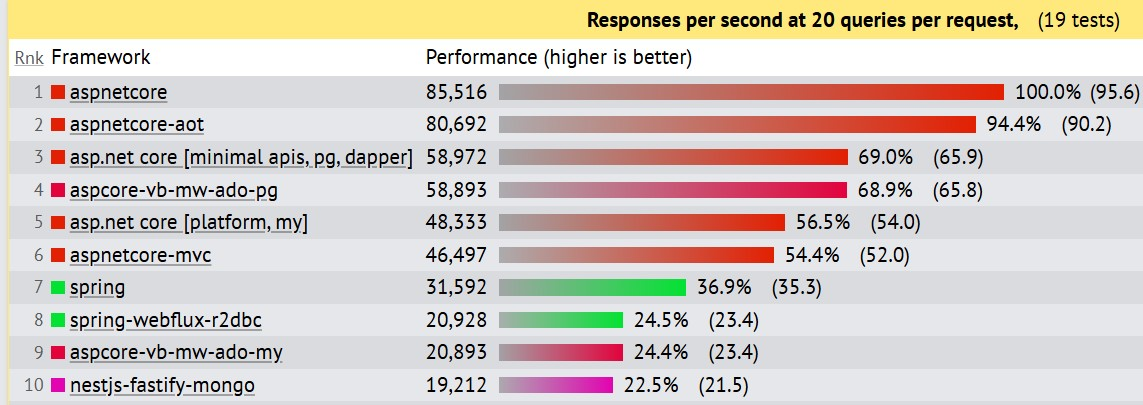
\includegraphics[width=\textwidth]{Graphics/Cap2/bencharmk_definitivo.jpg}
        \textbf{(a)} Tasa de transferencia (respuestas por segundo)
    \end{minipage}
    \hfill
    \begin{minipage}[b]{0.48\textwidth}
        \centering
        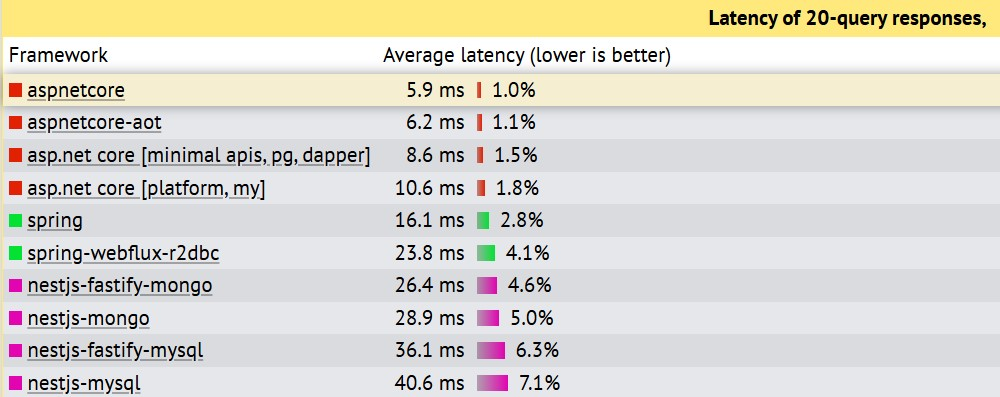
\includegraphics[width=\textwidth]{Graphics/Cap2/latencia.jpg}
        \textbf{(b)} Tiempo de procesamiento para 20 consultas
    \end{minipage}
    \caption{Comparación de rendimiento entre .NET, Spring Boot y Node.js en el escenario de 20 consultas por solicitud (adaptado de TechEmpower Framework Benchmarks \cite{techempower_benchmarks})}
    \label{fig:benchmark_rendimiento}
\end{figure}



\subsubsection{Selección de la plataforma}

A partir del análisis realizado, .NET constituye la opción más adecuada para el sistema de farmacovigilancia por las siguientes razones:

\begin{enumerate}
    \item \textbf{Eficiencia de recursos:} menor consumo de memoria y alto rendimiento bajo carga, lo que favorece su despliegue en entornos con recursos limitados \cite{performance_study}.
    \item \textbf{Fiabilidad en operación:} comportamiento estable bajo cargas sostenidas, que garantiza la integridad de las transacciones críticas \cite{performance_study}.
    \item \textbf{Ecosistema integrado:} proporciona bibliotecas nativas para seguridad, persistencia y autenticación, lo que evita la dependencia de componentes externos y facilita la evolución del sistema con soporte a largo plazo.
    \item \textbf{Adecuación al contexto:} la experiencia previa con el ecosistema .NET reduce la curva de aprendizaje y el riesgo de implementación.
\end{enumerate}

\subsection{Tecnologías para el desarrollo de la interfaz de usuario}
\label{subsection:frontend}

El análisis considera tres tecnologías representativas del desarrollo de interfaces de usuario modernas: React, Angular y Vue. La selección de estas tres responde a que representan enfoques distintos dentro del ecosistema actual —una biblioteca flexible, un framework integral y un marco progresivo—, lo que permite una comparación basada en los criterios definidos.

\subsubsection{React}

React es una biblioteca de JavaScript desarrollada por Meta para la construcción de interfaces mediante componentes reutilizables. 
Su modelo declarativo opera sobre una representación virtual del documento (Virtual DOM). En lugar de manipular directamente la estructura del navegador, React aplica los cambios sobre esta representación virtual. A continuación, un algoritmo de reconciliación calcula la diferencia mínima con el estado anterior y actualiza solo los elementos modificados.
Esta estrategia reduce las operaciones costosas de manipulación del documento y mejora el rendimiento en interfaces con alta frecuencia de cambios \cite{react_official}. 
React no impone una estructura completa; el enrutamiento y la gestión de estado recaen en bibliotecas externas, lo que otorga flexibilidad a costa de una mayor dependencia del ecosistema.

\subsubsection{Angular}

Angular es un framework de desarrollo de interfaces de usuario basado en TypeScript, mantenido por Google. 
Utiliza un mecanismo de vinculación bidireccional que sincroniza automáticamente el modelo de datos con la vista sin necesidad de manipulación manual \cite{angular_official}.
A diferencia de React, Angular constituye una solución integral que incluye enrutamiento, inyección de dependencias, manejo de formularios y herramientas de estructuración. 
Su enfoque dirigido por convenciones define una arquitectura estandarizada desde el inicio del proyecto, lo que favorece la consistencia en aplicaciones de gran escala pero incrementa la curva de aprendizaje.

\subsubsection{Vue}

Vue.js es un framework progresivo de JavaScript diseñado para la construcción de interfaces interactivas. 
Su sistema de reactividad rastrea automáticamente las dependencias entre los datos y la vista, actualizando solo los componentes afectados cuando el estado cambia \cite{vue_official}. 
Su diseño incremental permite adoptarlo de forma gradual: puede integrarse en proyectos existentes como una biblioteca ligera o utilizarse como framework completo, lo que reduce la curva de aprendizaje inicial.
Su reducido tamaño lo hace adecuado para cargas rápidas en redes con conectividad limitada.

\subsubsection{Comparación de los frameworks de interfaz de usuarios}

La Tabla \ref{tab:comparacion_frontend} resume la comparación realizada según los criterios definidos en la Sección~\ref{subsection:criterios}. 
En la interfaz de usuario, la eficiencia corresponde a la velocidad de actualización de la vista, la escalabilidad a la gestión de componentes complejos, y la mantenibilidad a la estructura del código.

\begin{table}[htbp]
	\centering
	\caption{Comparación de tecnologías para la interfaz de usuario según criterios de evaluación}
	\label{tab:comparacion_frontend}
	\renewcommand{\arraystretch}{1.3}
	\begin{tabular}{p{3.2cm} p{3.5cm} p{3.5cm} p{3.5cm}}
	\textbf{Criterio} & \textbf{React} & \textbf{Angular} & \textbf{Vue} \\[6pt]
		Eficiencia & Alta (representación virtual, actualización selectiva) & Media (detección de cambios por zonas) & Alta (reactividad basada en dependencias) \\ \hline
		Escalabilidad & Alta (componentes reutilizables) & Muy alta (arquitectura modular integrada) & Alta (composición flexible) \\ \hline
		Mantenibilidad & Alta (ecosistema flexible) & Muy alta (estructura tipada integral) & Alta (estructura progresiva) \\ \hline
		Curva de aprendizaje & Media (dependencia de bibliotecas externas) & Alta (framework integral) & Baja-Media (adopción gradual) \\ \hline
		Madurez & Muy alta (respaldada por Meta, amplia comunidad) & Muy alta (uso empresarial consolidado) & Alta (comunidad activa, ecosistema en crecimiento) \\ \hline
	\end{tabular}
\end{table}


\subsubsection{Selección del framework de interfaz de usuario}

Considerando los criterios evaluados, React presenta un equilibrio entre eficiencia, flexibilidad y mantenibilidad. Su modelo basado en componentes reutilizables y su estrategia de actualización selectiva lo hacen adecuado para interfaces con formularios dinámicos como los requeridos por el sistema de farmacovigilancia. Su ecosistema de bibliotecas externas permite cubrir los requisitos de validación, visualización de datos y diseño responsivo sin la rigidez estructural de Angular ni la menor madurez de Vue. Por estas razones, React constituye la tecnología seleccionada para el desarrollo de la interfaz de usuario.

\subsection{Sistemas de gestión de bases de datos}
\label{subsection:bases_datos}

Un sistema de gestión de bases de datos (SGBD) es un software encargado de gestionar el almacenamiento, la organización y la consulta de grandes volúmenes de información. 
Para el sistema de farmacovigilancia, el análisis aborda primero los dos paradigmas predominantes —relacional y no relacional— y posteriormente los gestores concretos dentro del paradigma seleccionado.

\begin{itemize}
\item \textbf{Bases de datos relacionales:} organizan la información en tablas con esquema rígido y utilizan el lenguaje de consulta estructurado (SQL, del inglés Structured Query Language) para acceder a los datos. Cumplen las propiedades ACID, lo que garantiza la integridad de los datos en operaciones críticas \cite{elmasri2016fundamentals}.
\item \textbf{Bases de datos no relacionales (NoSQL, del inglés Not Only SQL):} operan con esquemas flexibles y priorizan la disponibilidad y el rendimiento sobre la consistencia inmediata, siguiendo el modelo BASE \cite{moniruzzaman2013nosql}. Son adecuadas para grandes volúmenes de datos no estructurados.
\end{itemize}


\begin{table}[htbp]
	\centering
	\caption{Comparación de paradigmas de bases de datos según criterios de evaluación}
	\label{tab:comparacion_db}
	\renewcommand{\arraystretch}{1.3}
	\begin{tabular}{p{3.2cm} p{6.0cm} p{6.0cm}}
	\textbf{Criterio} & \textbf{Relacional (SQL)} & \textbf{No Relacional (NoSQL)} \\[6pt]
		Estructura de datos & Tablas con columnas y filas & Modelos basados en documentos, pares clave-valor, familias de columnas o grafos \\ \hline
		Esquema & Esquema rígido (definido antes de la inserción de datos) \cite{elmasri2016fundamentals} & Esquema flexible (puede variar entre registros) \cite{moniruzzaman2013nosql} \\ \hline
		Escalabilidad & Verticalmente escalable (aumento de recursos hardware del nodo) & Horizontalmente escalable (agregando más nodos al sistema) \\ \hline
		Integridad de los datos & Cumple con ACID (alta consistencia) \cite{ibm_acid_properties} & Cumple con BASE (mayor disponibilidad, menor consistencia) \cite{ibm_cap_theorem} \\ \hline
		Rendimiento & Alto en consultas complejas y operaciones transaccionales & Alta en grandes volúmenes de datos y operaciones de lectura/escritura rápidas \\ \hline
		Curva de aprendizaje & Media (requiere modelado relacional, normalización y dominio de SQL) & Media-Baja (menor necesidad de esquemas rígidos) \\ \hline
	\end{tabular}
\end{table}

En el sistema de farmacovigilancia, la prioridad es la integridad de la información clínica, no el manejo de grandes volúmenes de datos no estructurados. 
Las propiedades ACID de las bases de datos relacionales aseguran que cada operación concluya sin inconsistencias, lo que resulta esencial cuando los datos alimentan directamente la toma de decisiones clínicas.
Por esta razón, el paradigma relacional constituye la base del sistema. 
Las bases de datos no relacionales mantienen su vigencia para escenarios complementarios —documentos, evidencias, fotografías o mecanismos de almacenamiento en caché— donde la flexibilidad de esquema y el rendimiento en lectura predominan sobre la consistencia transaccional.

\subsubsection{Comparación de gestores de bases de datos relacionales}

Una vez seleccionado el paradigma relacional, el análisis compara tres gestores —MySQL, PostgreSQL y SQL Server— que comparten un perfil adecuado para aplicaciones web multiusuario: todos operan como servicio independiente, admiten concurrencia y ofrecen integración con .NET \cite{microsoft_sql_comparison}. 

La comparación valora cuatro criterios, resumidos en la Tabla \ref{tab:comparacion_sql}: 
La integración con .NET determina la facilidad de conexión entre el gestor y el framework de desarrollo elegido, y evita configuraciones adicionales.
La licencia condiciona la viabilidad económica del proyecto: una licencia comercial introduce costos que una solución de código abierto elimina. 
El despliegue multiplataforma garantiza que el sistema pueda trasladarse entre entornos sin cambios en la configuración. 
La curva de aprendizaje influye en la velocidad con que un desarrollador puede dominar la administración del gestor \cite{microsoft_sql_comparison}. 


\begin{table}[H]
	\centering
	\caption{Comparación de gestores de bases de datos relacionales}
	\label{tab:comparacion_sql}
	\renewcommand{\arraystretch}{1.3}
	\begin{tabular}{p{2.8cm} p{3.2cm} p{3.2cm} p{3.2cm} p{3.2cm}}
	\textbf{Criterio} & \textbf{MySQL} & \textbf{PostgreSQL} & \textbf{SQL Server}  \\[6pt]
		Integración con .NET & Alta (Pomelo) & Alta (Npgsql) & Nativa (Microsoft)  \\ \hline
		Rendimiento & Alto en lectura & Alto en consultas complejas & Alto, optimizado para .NET  \\ \hline
		Licencia & Código abierto (GPL) & Código abierto (PostgreSQL) & Comercial (Microsoft)  \\ \hline
		Despliegue & Multiplataforma & Multiplataforma & Principalmente Windows \\ \hline
		Curva de aprendizaje & Media & Media-Alta & Media \\ \hline
	\end{tabular}
\end{table}


SQL Server ofrece la integración más natural con .NET y Entity Framework por pertenecer al mismo ecosistema Microsoft, lo que aporta soporte nativo, documentación unificada y herramientas de desarrollo integradas. 
Sin embargo, su licencia comercial introduce costos difíciles de justificar para un proyecto en fase de desarrollo, y su dependencia del entorno Windows limita la portabilidad del sistema. 

PostgreSQL ofrece la mayor potencia en consultas complejas y un ecosistema de extensiones que lo hacen preferible para aplicaciones con requisitos analíticos avanzados, aunque esta capacidad adicional incrementa su curva de aprendizaje y el consumo de recursos. 

MySQL, aunque no alcanza la integración nativa de SQL Server ni la potencia analítica de PostgreSQL, ofrece un equilibrio adecuado para el sistema de farmacovigilancia: un proveedor consolidado para .NET (Pomelo), una licencia de código abierto que elimina los costos de licenciamiento, una compatibilidad multiplataforma que facilita el despliegue en cualquier entorno y una imagen de contenedor ligera que reduce el consumo de recursos durante el desarrollo. 
Por estas razones, MySQL constituye el gestor seleccionado para el sistema.

% \subsection{Otras herramientas y librerías}

% % hablaremos de las librerias de react para desarrollar graficos y formulario dinamicos
% % hablaremos de las librerias de net para manejar bases de datos, para manejar seguridad
% % alternativas de captcha entre Friendly Captcha, Google ReCaptcha y las de imágenes



\section{Conclusiones del capítulo}
\label{section:conclusiones_estado_arte}

El presente capítulo estableció los fundamentos conceptuales y tecnológicos que sustentan el desarrollo del sistema de farmacovigilancia. El análisis del estado del arte identificó las brechas de los sistemas existentes y permitió extraer directrices de diseño que orientan la solución propuesta. Los fundamentos de sistemas web definieron la arquitectura cliente-servidor como modelo organizativo, y los fundamentos de bases de datos justificaron la elección del paradigma relacional a partir de las propiedades ACID.

El análisis comparativo de tecnologías permitió seleccionar el conjunto de herramientas que materializará el sistema. Para la capa de servicios, .NET ofreció el mejor equilibrio entre eficiencia, mantenibilidad y adecuación al contexto de desarrollo. Para la interfaz de usuario, React aportó flexibilidad y un ecosistema compatible con los requisitos del sistema. Para la persistencia, MySQL proporcionó una solución de código abierto, multiplataforma y con integración consolidada con .NET. Estas decisiones constituyen la base tecnológica sobre la cual el Capítulo \ref{chapter:proposal} desarrolla el diseño del sistema.
%\chapter{Metodología y Análisis del Sistema Propuesto:}\label{chapter:proposal}

¿Cómo se va a construir el sistema y por qué se eligió esta forma?


\section{Metodologías de desarrollo de software}
\label{section:metodologias_desarrollo}

Una metodología de desarrollo de software es un marco de trabajo estructurado que organiza, planifica y controla el proceso de construcción de un sistema. Su relevancia radica en que permite reducir la complejidad del desarrollo al dividir el proyecto en etapas gestionables, establecer un lenguaje común entre los involucrados y mejorar la calidad del producto final mediante prácticas sistemáticas de ingeniería de software \cite{Pfleeger2015}.

En este contexto, existen diversas metodologías de desarrollo, cada una con enfoques particulares para la gestión del ciclo de vida del software.

\begin{itemize}

\item El modelo en cascada se basa en un enfoque secuencial y lineal del desarrollo, donde las fases de análisis, diseño, implementación, pruebas y mantenimiento se ejecutan de manera ordenada y progresiva. Cada fase debe completarse antes de iniciar la siguiente, lo que proporciona un alto nivel de control y documentación, aunque limita la flexibilidad ante cambios durante el desarrollo \cite{Sommerville2015, Royce1987}.

\item Scrum es un marco de trabajo ágil basado en el desarrollo iterativo e incremental, en el cual el sistema se construye mediante ciclos cortos llamados \textit{sprints}. Cada iteración produce un incremento funcional del sistema, permitiendo la adaptación continua a cambios y la inspección constante del progreso \cite{Schwaber2020}.

\item Kanban es un método de gestión del flujo de trabajo orientado a la mejora continua del proceso de desarrollo. Se basa en la visualización del trabajo, la limitación del trabajo en curso y la optimización del flujo de tareas, permitiendo una entrega continua sin necesidad de iteraciones fijas \cite{Anderson2010}.

\item Extreme Programming (XP) es una metodología ágil centrada en la calidad técnica del software. Se fundamenta en valores como la simplicidad, la comunicación y la retroalimentación constante, e incorpora prácticas como el desarrollo guiado por pruebas, la refactorización continua y la programación en parejas, con el objetivo de mejorar la mantenibilidad y robustez del sistema \cite{Beck2004}.

\end{itemize}


\subsection{Comparación de metodologías de desarrollo aplicadas al sistema}
\label{subsection:comparacion_metodologias_sistema}

Con el objetivo de seleccionar la metodología más adecuada para el desarrollo del sistema de gestión y autorreporte de ESAVI , se realizó un análisis comparativo entre los diferentes enfoques de desarrollo de software, evaluando su comportamiento en relación con las características específicas del proyecto.

Entre los criterios considerados se incluyen la variabilidad de los requisitos, la necesidad de desarrollo incremental, la mantenibilidad del código, la compatibilidad con una arquitectura desacoplada, la capacidad de adaptación a cambios en el diseño y la resiliencia ante interrupciones operativas durante el desarrollo, tales como cortes de energía eléctrica y problemas de conectividad.


\begin{table}[h!]
\centering
\renewcommand{\arraystretch}{1.3}
\begin{tabular}{|p{3.5cm}|p{2.8cm}|p{2.8cm}|p{2.8cm}|p{2.8cm}|}
\hline
\textbf{Criterio} & \textbf{Cascada} & \textbf{Scrum} & \textbf{Kanban} & \textbf{XP} \\
\hline

Flexibilidad ante cambios de requisitos y rediseño 
& Baja. Enfoque secuencial con poca capacidad de adaptación una vez avanzadas las fases. 
& Alta. Permite adaptación iterativa de requisitos y ajustes entre entregas. 
& Alta. Facilita la reorganización continua de tareas y prioridades. 
& Alta. Soporta cambios mediante refactorización continua y desarrollo incremental. \\
\hline

Calidad y mantenibilidad del código 
& Baja. No incorpora prácticas técnicas específicas de calidad. 
& Media. Depende de las prácticas del equipo de desarrollo. 
& Baja. No influye directamente en la calidad del código. 
& Alta. Promueve refactorización, simplicidad y buenas prácticas de desarrollo. \\
\hline

Soporte para arquitectura modular (Clean Architecture) 
& Baja. Diseño rígido definido al inicio con poca adaptabilidad. 
& Alta. Permite evolución progresiva de la arquitectura. 
& Media. No define estructura arquitectónica. 
& Alta. Favorece la separación de responsabilidades y modularidad del sistema. \\
\hline

Adecuación al contexto de desarrollo individual y restricciones operativas 
& Baja. Requiere planificación rígida y secuencial. 
& Media. Diseñado para equipos, requiere adaptación en contexto individual. 
& Alta. Flexible y adecuado para gestión individual de tareas. 
& Alta. Compatible con desarrollo individual y mejora continua del código. \\
\hline

\end{tabular}
\caption{Comparación de metodologías de desarrollo según criterios del sistema}
\label{tab:comparacion_metodologias_4criterios}
\end{table}

\subsection{Aplicación Práctica de Scrum en el Proyecto}

Para el desarrollo del sistema de autorreporte de ESAVI se seleccionó Scrum por su flexibilidad para gestionar entregas incrementales y adaptarse a cambios en los requisitos, decisión respaldada por la experiencia previa del autor, las tutoras y el equipo revisor del Instituto Finlay de Vacunas en metodologías ágiles. Dado el carácter unipersonal del proyecto, el desarrollador asumió los roles de \textit{Scrum Master} y Equipo de Desarrollo, mientras que las tutoras oficiaron como \textit{Product Owner}, definiendo requisitos y validando entregas sin intervenir en aspectos técnicos \cite{Schwaber2020}.


El trabajo se estructuró en \textbf{cuatro \textit{Sprints}} de dos semanas. Antes de cada uno, se realizaba una \textit{Sprint Planning} donde las tutoras comunicaban las prioridades y se acordaban el objetivo y las tareas del ciclo. Durante la iteración, el progreso se controlaba mediante un tablero Kanban. Las funcionalidades desarrolladas fueron:
\begin{itemize}
    \item \textbf{\textit{Sprint} 1:} Arquitectura base y formulario de autorreporte con datos del paciente, vacuna administrada y tipo de evento adverso.
    \item \textbf{\textit{Sprint} 2:} Anonimización de datos y almacenamiento seguro de reportes.
    \item \textbf{\textit{Sprint} 3:} Panel de seguimiento de casos notificados para profesionales de salud.
    \item \textbf{\textit{Sprint} 4:} Refinamiento de interfaz, validaciones clínicas y preparación para despliegue.
\end{itemize}
Al cierre de cada \textit{Sprint}, se efectuaba una \textit{Sprint Review} con las tutoras para verificar el cumplimiento de requisitos y plazos, y una \textit{Sprint Retrospective} individual para ajustar el proceso. Esta dinámica permitió incorporar, desde el segundo ciclo, nuevos criterios de clasificación de eventos adversos de la OMS sin afectar la fecha de entrega \cite{Schwaber2020}.

\section{Levantamiento y análisis de requisitos}
\label{section:requisitos}

En esta sección se presentan los requisitos del sistema, obtenidos a partir del análisis del flujo de farmacovigilancia del Instituto Finlay de Vacunas. Se clasifican en requisitos funcionales —las acciones que el sistema debe realizar— y no funcionales —los atributos de calidad bajo los cuales debe operar—.

\subsection{Requisitos funcionales}
\label{subsection:requisitos_funcionales}

El sistema web de autorreporte de \gls{esavi} se centra en la captura, gestión y seguimiento de reportes, así como en el soporte al análisis de la información por parte del personal autorizado. A continuación, se describen los principales requerimientos funcionales:

\begin{itemize}

\item \textbf{RF-01. Registro de eventos adversos:}  
El sistema deberá permitir a los usuarios registrar reportes de eventos adversos post-vacunación mediante un formulario web estructurado.

\item \textbf{RF-02. Gestión de información del reporte:}  
El sistema deberá permitir la captura de datos del paciente, vacunas administradas, y descripción del evento adverso, incluyendo la posibilidad de registrar múltiples eventos en un mismo reporte.

\item \textbf{RF-03. Identificación del reporte:}  
El sistema deberá generar automáticamente un código único de notificación o identificación para cada reporte registrado exitosamente.

\item \textbf{RF-04. Validación de formularios:}  
El sistema deberá validar los campos obligatorios del formulario antes de permitir el envío del reporte.

\item \textbf{RF-05. Almacenamiento de reportes:}  
El sistema deberá almacenar los reportes en una base de datos centralizada para su posterior análisis y seguimiento.

\item \textbf{RF-06. Gestión del estado del reporte:}  
El sistema deberá permitir la actualización del estado de los reportes dentro del flujo de farmacovigilancia (por ejemplo: pendiente, en revisión, validado, cerrado).

\item \textbf{RF-07. Consulta y filtrado de reportes:}  
El sistema deberá permitir la búsqueda y filtrado de reportes según criterios como fecha, vacuna, severidad y datos demográficos.

\item \textbf{RF-08. Visualización de información:}  
El sistema deberá permitir la visualización detallada de cada reporte de evento adverso.

\item \textbf{RF-09. Gestión de usuarios:}  
El sistema deberá permitir la autenticación de usuarios y la administración de roles para el acceso a funcionalidades específicas.

\item \textbf{RF-10. Generación de estadísticas:}  
El sistema deberá generar reportes estadísticos y visualizaciones gráficas para el análisis de los eventos adversos registrados.

\item \textbf{RF-11. Exportación de datos:}  
El sistema deberá permitir la exportación de información en formatos utilizados para análisis o reporte institucional.

\item \textbf{RF-12. Notificaciones del sistema:}  
El sistema deberá generar notificaciones automáticas basadas en eventos del flujo de gestión de reportes de eventos adversos, dirigidas a los usuarios según su rol dentro del sistema.

\end{itemize}

\subsection{Requerimientos no funcionales del sistema}
\label{subsection:requerimiento_no_funcionales}

El sistema web de autorreporte de eventos adversos post-vacunación deberá cumplir con un conjunto de requerimientos no funcionales orientados a garantizar la calidad, seguridad, disponibilidad y usabilidad de la plataforma.

\begin{itemize}

\item \textbf{RNF-01 Eficiencia y usabilidad del registro.}  
El sistema deberá cumplir con los siguientes criterios en el proceso de reporte de un evento adverso:
\begin{itemize}
    \item Completarse en un tiempo promedio menor a 2 minutos por parte de un usuario familiarizado con la plataforma.
    \item Presentar una interfaz intuitiva\footnote{Se entiende por interfaz intuitiva aquella que puede ser utilizada sin entrenamiento previo, siguiendo patrones de diseño web convencionales reconocidos por el usuario promedio.} y fácil de usar para usuarios con diferentes niveles de alfabetización digital.
    \item Basar la captura de datos principalmente en elementos estructurados como listas desplegables, botones de selección y casillas de verificación, minimizando el uso de texto libre.
\end{itemize}

\item \textbf{RNF-02. Accesibilidad:}  
El sistema deberá cumplir con las pautas de accesibilidad WCAG 2.1\footnote{Web Content Accessibility Guidelines (WCAG) 2.1: estándar internacional que establece criterios para hacer el contenido web accesible a personas con discapacidad visual, auditiva, motriz y cognitiva. El nivel AA es el umbral recomendado para sitios web gubernamentales y de salud.} nivel AA, garantizando su uso por personas con diferentes capacidades físicas y sensoriales.

\item \textbf{RNF-03. Diseño responsivo:}  
El sistema deberá adaptarse adecuadamente a diferentes dispositivos y resoluciones de pantalla, incluyendo computadoras de escritorio, tabletas y dispositivos móviles.

\item \textbf{RNF-04 Rendimiento.}  
El sistema deberá cargar sus páginas en un tiempo inferior a 3 segundos y procesar el envío de un reporte en menos de 5 segundos bajo condiciones normales de conectividad.

\item \textbf{RNF-05. Seguridad de la información:}  
El sistema deberá garantizar la confidencialidad, integridad y disponibilidad de los datos mediante mecanismos de autenticación, control de acceso y cifrado de información sensible.

\item \textbf{RNF-06. Auditoría y trazabilidad:}  
El sistema deberá registrar las acciones relevantes realizadas por los usuarios, incluyendo creación, modificación y actualización de reportes, con fines de auditoría y control institucional.

\item \textbf{RNF-07 Mantenibilidad.}  
El sistema deberá estar diseñado de manera modular, con separación clara entre sus componentes, facilitando la corrección de errores, la incorporación de nuevas funcionalidades y la escalabilidad del sistema.

\item \textbf{RNF-08. Compatibilidad:}  
El sistema deberá ser compatible con los principales navegadores web modernos: Google Chrome, Mozilla Firefox, Microsoft Edge y Safari.

\end{itemize}

\subsection{Reglas de negocio}
\label{subsection:reglas_negocio}

A continuación se describen las reglas que rigen la lógica de los formularios y el procesamiento de reportes dentro del sistema:

\begin{itemize}

\item \textbf{RN-01 Unicidad de vacuna por fecha.} No se puede registrar la misma vacuna más de una vez en la misma fecha para un mismo sujeto vacunado.

\item \textbf{RN-02 Vacunación previa al evento.} La fecha del primer evento adverso reportado debe ser siempre posterior a la fecha de la vacunación más reciente registrada en el reporte.

\item \textbf{RN-03 Eventos posteriores al fallecimiento.} Si en alguno de los eventos adversos se declara como desenlace el fallecimiento del sujeto vacunado, no se permitirá registrar nuevos eventos adversos con fecha posterior a la fecha de muerte.

\end{itemize}

\section{Modelado del sistema}

\subsection{Diagrama de casos de uso}

En esta sección se exponen las acciones que pueden realizar los distintos tipos de usuarios dentro de la plataforma, detalladas a través de un diagrama de casos de uso\footnote{Diagrama de casos de uso: Forma de diagrama de comportamiento UML mejorado. Sirve para especificar la comunicación y el comportamiento de un sistema mediante su interacción con los usuarios y/u otros sistemas.}. 
Para una mejor comprensión, se han categorizado las funcionalidades según el rol del actor y las dependencias lógicas de inclusión y extensión que rigen el sistema.

\subsubsection{Identificación de Actores}

De acuerdo con el modelado funcional, se han identificado cinco actores principales que interactúan con el sistema de gestión de vacunación y \gls{esavi}:

\begin{itemize}
    \item \textbf{Usuario:} Actor abstracto que representa la base de permisos comunes. De él heredan todos los roles que requieren autenticación en el sistema.
    \item \textbf{Jefe de Vacunación Municipal:} Hereda de Usuario. Responsable de la supervisión local, encargado de la gestión del personal médico y la distribución de la carga de trabajo.
    \item \textbf{Médico Evaluador:} Hereda de Usuario. Profesional sanitario encargado del análisis clínico de los eventos reportados.
    \item \textbf{Administrador:} Hereda de Usuario. Perfil técnico responsable del mantenimiento de los parámetros del sistema (catálogos) y la gestión de usuarios de alto nivel.
    \item \textbf{Reportante:} Actor independiente sin autenticación. Encargado de la entrada inicial de datos y el seguimiento de los reportes generados mediante el número de notificación.
\end{itemize}

\subsubsection{Análisis de los Casos de Uso}
A continuación, se describen las funcionalidades principales representadas en la Figura \ref{fig:diagrama_casos_uso}, detallando la lógica de negocio asociada a cada interacción:

\begin{figure}[H]
    \centering
    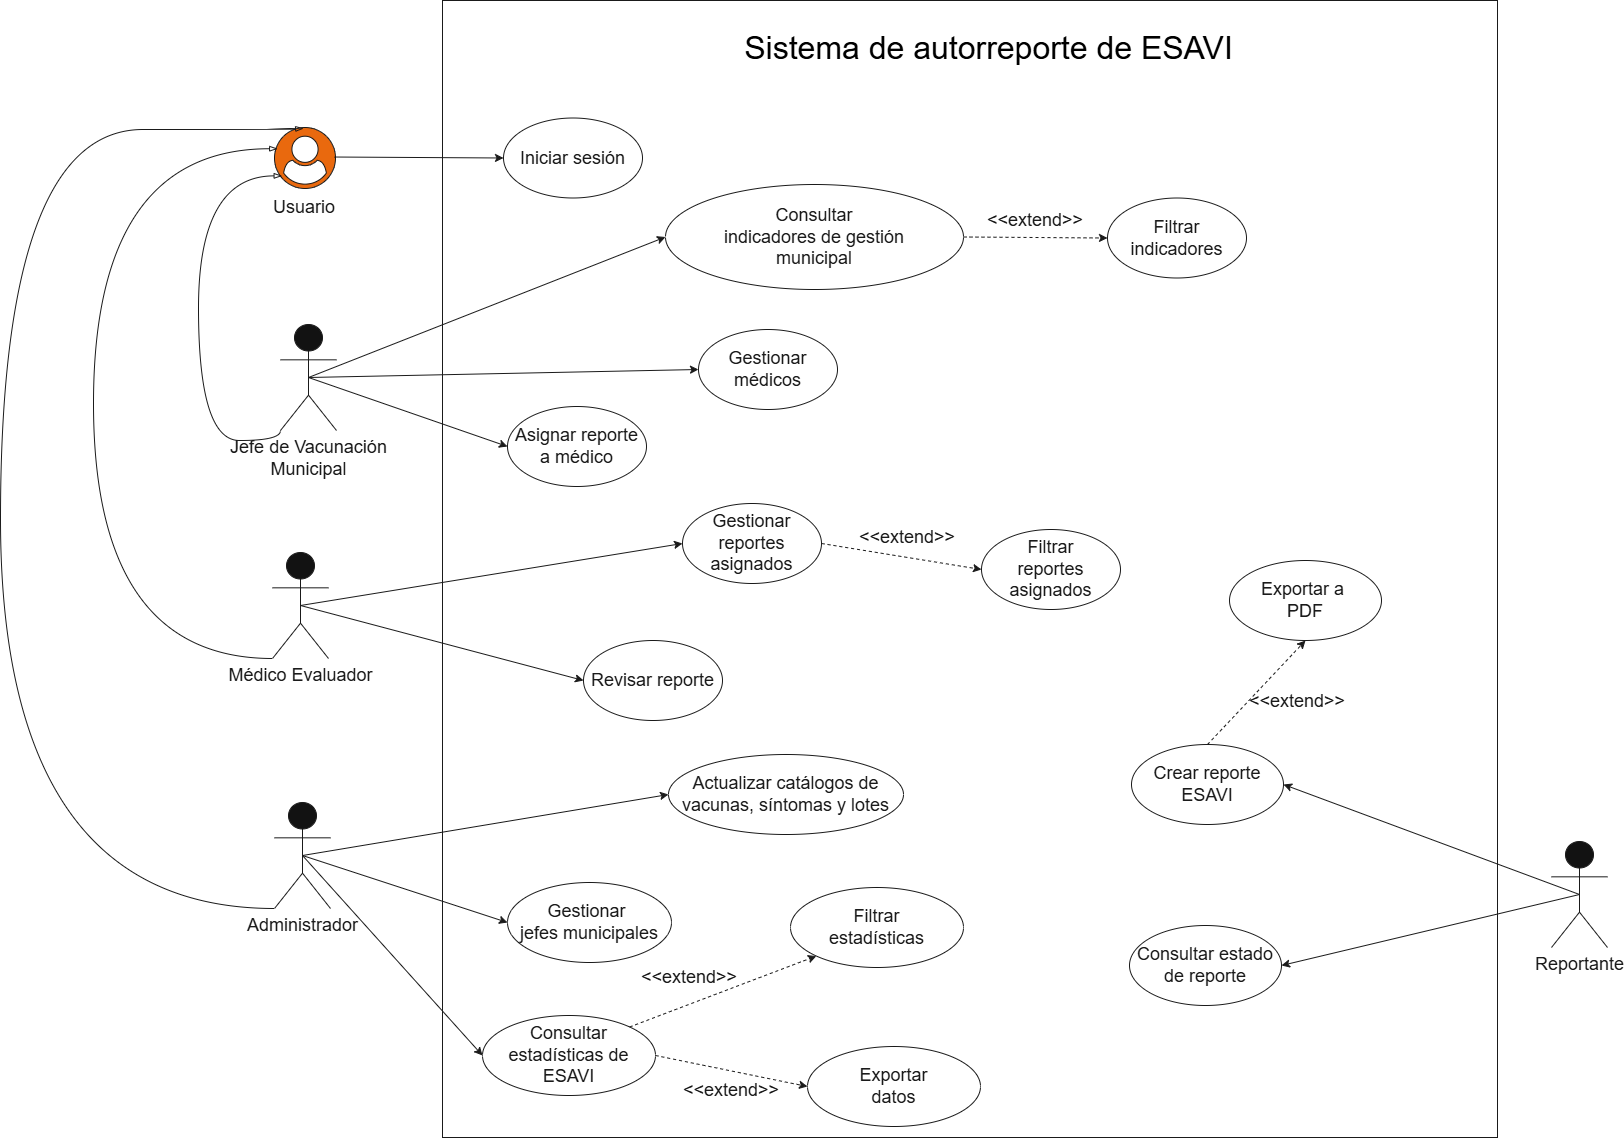
\includegraphics[scale=0.2]{Graphics/Cap3/diagrama_casos_uso_white.drawio (4).png}
    \caption[Diagrama de casos de uso]{Diagrama de casos de usos. Fuente: elaboración propia.}
    \label{fig:diagrama_casos_uso}
\end{figure}


\begin{itemize} 
    \item \textbf{Iniciar sesión:} Caso de uso base que permite el acceso controlado a la plataforma según las credenciales del usuario.
    \item \textbf{Gestión de reportes (Reportante):}
        \begin{itemize}
            \item \textbf{Crear reporte ESAVI:} Permite el ingreso de un nuevo evento adverso. Este caso de uso posee una relación de tipo \textit{extend} hacia \textbf{Exportar a PDF}, lo que indica que el usuario puede, opcionalmente, generar un comprobante documental tras completar el registro.
            \item \textbf{Consultar estado de reporte:} Permite al reportante verificar el estado de sus envíos previos ingresando el número de notificación.
        \end{itemize}

    \item \textbf{Gestión Clínica (Médico Evaluador):}
    \begin{itemize}
        \item \textbf{Gestionar reportes asignados:} Vista principal del médico donde visualiza su carga laboral. De manera opcional (\textit{extend}), puede aplicar \textbf{Filtrar reportes asignados} para priorizar por antigüedad, severidad u otros criterios.
        \item \textbf{Revisar reporte:} Acción de análisis detallado de la información clínica para determinar la causalidad del evento.
    \end{itemize}

    \item \textbf{Supervisión Municipal (Jefe de Vacunación):}
    \begin{itemize}
        \item \textbf{Asignar reporte a médico:} Funcionalidad crítica para delegar los casos entrantes al personal evaluador disponible.
        \item \textbf{Consultar indicadores de gestión municipal:} Permite al jefe municipal visualizar un panel con métricas clave para la toma de decisiones, tales como carga de trabajo por médico, porcentaje de reportes completados, tiempos promedio de respuesta y congestión del flujo de trabajo. De manera opcional (\textit{extend}), puede aplicar \textbf{Filtrar indicadores} para segmentar los datos por período, médico, estado del reporte y la severidad.
        \item \textbf{Gestionar médicos:} Permite el alta, baja y modificación de los perfiles médicos bajo su jurisdicción.
    \end{itemize}

    \item \textbf{Administración y Configuración (Administrador):}
    \begin{itemize}
        \item \textbf{Actualizar catálogos:} Garantiza que la información de vacunas, síntomas y lotes se mantenga vigente.
        \item \textbf{Gestionar jefes municipales:} Permite el alta, baja y modificación de las cuentas de los jefes de vacunación municipal.
        \item \textbf{Consultar estadísticas de ESAVI:} Permite al administrador visualizar un panel con indicadores agregados de los eventos adversos reportados, como número de reportes por vacuna, lote, región, municipio o nivel de severidad. De manera opcional, permite aplicar \textbf{Filtrar estadísticas} (\textit{extend}) para segmentar los datos y \textbf{Exportar datos} (\textit{extend}) en formatos PDF o Excel para análisis externos.
    \end{itemize}
\end{itemize}



\subsection{Diagramas de secuencia}

\subsection{Modelo de dominio}


\section{Arquitectura del sistema}
\label{section:arquitectura}

La arquitectura de software se define como la estructura o conjunto de estructuras del sistema, que comprende los elementos de software, sus propiedades visibles externamente y las relaciones entre ellos \cite{bass2021}. Es el plano conceptual que define la organización fundamental del sistema.

Su importancia para este proyecto radica en su rol como habilitador de atributos de calidad críticos. Una arquitectura bien definida permite razonar y gestionar cambios futuros (como nuevas regulaciones de farmacovigilancia), anticipar el cumplimiento de propiedades como seguridad o mantenibilidad, y establecer una base común de comunicación entre los interesados (desarrolladores, personal médico y entes regulatorios) \cite{bass2021}.


\subsection{Monolito vs Microservicios}
\label{subsection: monolito_vs_microservicios}

\begin{itemize}
    \item \textbf{Arquitectura Monolítica:} Es el modelo tradicional donde toda la funcionalidad del software se construye como una única unidad con una sola base de código \cite{ibm_microservices_monolith}. Todos sus componentes (interfaz de usuario, lógica de negocio y acceso a datos) están estrechamente acoplados e interdependientes \cite{aws_monolith_microservices}.
    \item \textbf{Arquitectura de Microservicios:} Descompone la aplicación en una colección de servicios pequeños, autónomos y débilmente acoplados \cite{ibm_microservices_advantages}. Cada servicio se encarga de una función de negocio específica, tiene su propia base de datos y se comunica con otros mediante APIs (normalmente HTTP/REST) \cite{aws_monolith_microservices}. 
\end{itemize}

\begin{table}[htbp]
	\centering
	\label{tab:monolito_microservicios}
	
	\renewcommand{\arraystretch}{1.3}
	
	\begin{tabular}{p{3.2cm} p{4.3cm} p{4.3cm}}
		
		\textbf{Características} & \textbf{Monolito} & \textbf{Microservicios}\\[6pt]
		
		Unidad de despliegue &
	    Única (un solo archivo ejecutable) \cite{ibm_microservices_monolith} &
		Múltiple (cada servicio es independiente) \cite{aws_monolith_microservices} \\[6pt]
		\hline

		Complejidad Operativa &
        Baja; fácil de gestionar inicialmente. \cite{ibm_microservices_monolith} &
		Alta; requiere orquestación y monitoreo complejo \cite{aws_monolith_microservices}\\[6pt]
        \hline
		
		Depuración &
		Sencilla; flujo de datos en un mismo entorno \cite{ibm_microservices_monolith} &
		Difícil; requiere rastrear datos entre múltiples servicios \cite{aws_monolith_microservices}.  \\[6pt]
        \hline
		
		
	Escalabilidad
	& Se escala toda la aplicación completa \cite{ibm_microservices_monolith}
	& Se escala cada servicio según su demanda específica \cite{aws_monolith_microservices}
    
	\end{tabular}
\end{table}

Para el desarrollo del sistema de autorreporte de vacunas del Instituto Finlay, se determinó que la arquitectura monolítica es la opción más adecuada, especialmente considerando que el equipo de desarrollo inicial estuvo compuesto por un único integrante y que existían límites de tiempo estrictos para la entrega del producto. 
Las razones estratégicas se detallan a continuación:

\begin{itemize}
    \item \textbf{Rapidez de desarrollo (Time-to-Market):} En proyectos con cronogramas ajustados, el enfoque monolítico permite un desarrollo y despliegue mucho más ágil. 
    Al trabajar con una única base de código, se evita la complejidad y el tiempo adicional que supone coordinar múltiples servicios, interfaces de programación de aplicaciones (API) y fuentes de datos externas \cite{ibm_microservices_monolith}. 
    Esto permite al desarrollador centrarse en la lógica de negocio del reporte de ESAVI sin incurrir en la sobrecarga de diseño que exigen los microservicios.
    
    \item \textbf{Viabilidad para equipos de desarrollo reducidos:} Las fuentes indican que la arquitectura monolítica es ideal para equipos de desarrollo ajustados, ya que no impone una curva de aprendizaje excesivamente pronunciada ni requiere habilidades complejas de administración de sistemas distribuidos \cite{ibm_microservices_monolith}. 
    Para un solo desarrollador, gestionar una unidad de despliegue única simplifica drásticamente las tareas de codificación, pruebas de extremo a extremo y depuración, al poder rastrear el flujo de datos dentro de un mismo entorno de programación \cite{ibm_microservices_monolith}.
    
    \item \textbf{Eficiencia operativa y rendimiento técnico:} A diferencia de los microservicios, donde cada llamada entre componentes se convierte en una solicitud de red sujeta a latencia, congestión y fallos de comunicación, en un monolito las llamadas a funciones son instantáneas y predecibles \cite{docker_microservices_need}. 
    Se evitó así la sobrecarga innecesaria de serialización y deserialización de datos, garantizando un mejor desempeño en entornos donde los recursos de red e infraestructura pueden ser limitados \cite{ibm_microservices_monolith}.

\end{itemize}

Cabe destacar que la adopción de una arquitectura monolítica en la etapa inicial del sistema ESAVI no constituye una decisión irreversible, ni impide una eventual migración hacia microservicios \cite{aws_monolith_microservices}. 
Para que dicha transición sea viable sin requerir una reescritura completa del sistema, resulta imperativo aplicar desde el inicio patrones que favorezcan la modularidad y el bajo acoplamiento. 
Un monolito modular, diseñado con límites bien definidos entre sus componentes, permite que la extracción de un módulo hacia un servicio independiente sea un proceso incremental y de riesgo controlado, ya que las responsabilidades y los datos se encuentran lógicamente aislados desde su concepción \cite{docker_microservices_need}.

Con el propósito de alcanzar este nivel de preparación y asegurar la mantenibilidad a largo plazo, se evaluaron tres enfoques arquitectónicos para estructurar la lógica interna del sistema. Estos se introducen y comparan a continuación.

\subsection{Filosofías Candidatas}
\label{subsection:filosofia_candidatas}

\begin{itemize}
    \item \textbf{Arquitectura de N-Capas:} Su filosofía es dividir el sistema según responsabilidades técnicas. Consiste en organizar el código en estratos horizontales —presentación, lógica de negocio y acceso a datos— donde una capa solo puede invocar a la que está directamente debajo. Esto implica que la capa de negocio contiene referencias directas a la capa de base de datos, acoplando ambas \cite{microsoft_arch}.
    \item \textbf{Arquitectura Hexagonal (Puertos y Adaptadores):} Su filosofía es hacer que el núcleo de negocio ignore por completo los detalles externos. Consiste en colocar el dominio en el centro de la aplicación y rodearlo de puertos (interfaces que declaran lo que el dominio necesita del exterior) y adaptadores (implementaciones concretas de esas interfaces para tecnologías específicas como una base de datos o un sistema de correo). Así, cambiar de tecnología solo requiere escribir un nuevo adaptador, sin tocar el dominio \cite{cockburn2005, aws_hexagonal}.
    \item \textbf{Arquitectura Limpia (Clean Architecture):} Su filosofía es que las decisiones técnicas —frameworks, bases de datos, interfaces gráficas— sean detalles postergables que no afecten al núcleo del sistema. Consiste en disponer el código en anillos concéntricos: en el centro, las entidades de negocio con sus reglas; alrededor, los casos de uso que orquestan esas entidades; más afuera, los adaptadores que traducen formatos externos; y en la periferia, los frameworks. La regla es que una clase de un anillo exterior puede depender de una del interior, pero nunca al revés. Así, el dominio no sabe si los datos vienen de una API REST o de una línea de comandos \cite{martin2018}.
\end{itemize}

\begin{table}[h!]
\centering
\caption{Comparativa de arquitecturas según criterios del sistema de autorreporte ESAVI}
\label{tab:comparativa_esavi}
\begin{tabular}{|p{3.2cm}|p{3.5cm}|p{3.5cm}|p{3.5cm}|}
\hline
\textbf{Criterio} & \textbf{Arquitectura de N-Capas} & \textbf{Arquitectura Hexagonal} & \textbf{Arquitectura Limpia} \\
\hline
\textbf{Independencia de la infraestructura} & 
Baja. La capa de negocio referencia directamente a la capa de datos. Cambiar tecnología obliga a modificar la lógica \cite{microsoft_arch}. & 
Alta. El dominio define puertos; los adaptadores se reemplazan sin tocar el núcleo \cite{cockburn2005}. & 
Muy alta. Mismo principio que Hexagonal, con una regla de dependencia explícita que refuerza el aislamiento \cite{martin2018}. \cite{martin2018}. \\
\hline
\textbf{Testabilidad de la lógica clínica} & 
Baja. Probar una nueva función requiere instanciar la capa de datos o usar mocks complejos. & 
Alta. Los puertos permiten inyectar dobles de prueba directamente en el dominio. & 
Muy alta. El dominio no tiene dependencias; los casos de uso reciben interfaces que se simulan sin esfuerzo. \\
\hline
\textbf{Mantenibilidad ante cambios regulatorios} & 
Baja. Una modificación en las reglas de reporte obliga a revisar todas las capas. & 
Alta. Las reglas residen solo en el dominio; agregar o modificar no afecta los adaptadores \cite{cockburn2005}. & 
Alta. La división en Entidades y Casos de Uso indica exactamente dónde modificar: regla pura en Entidad, flujo en Caso de Uso \cite{martin2018}.\\
\hline
\end{tabular}
\end{table}

Con base en los resultados de la tabla, se seleccionó la Arquitectura Limpia. Esta satisface los criterios de independencia de la infraestructura, testabilidad y facilidad para agregar y mantener reglas de negocio, mientras que su diseño basado en interfaces permite intercambiar tecnologías —base de datos, proveedor de correo electrónico, sistema de notificaciones— sin modificar el núcleo del sistema. Asimismo, la regla de dependencia y la separación en anillos favorecen la aplicación de los principios \gls{SOLID} y DRY (ver glosario \gls{DRY}), al conducir naturalmente a clases con responsabilidades únicas, interfaces segregadas y lógica no duplicada \cite{martin2018}.


\subsection{Implementación de Arquitectura Limpia en el proyecto}
\label{subsection:clean_architecture}

La implementación de la Arquitectura Limpia en el sistema ESAVI se materializa en cuatro proyectos de .NET, cada uno correspondiente a un anillo de la arquitectura.
La Figura \ref{fig:arquitectura} ilustra esta organización: las dependencias entre proyectos reflejan estrictamente la regla de dependencia, apuntando únicamente hacia el centro.

\begin{figure}[htbp]
    \centering
    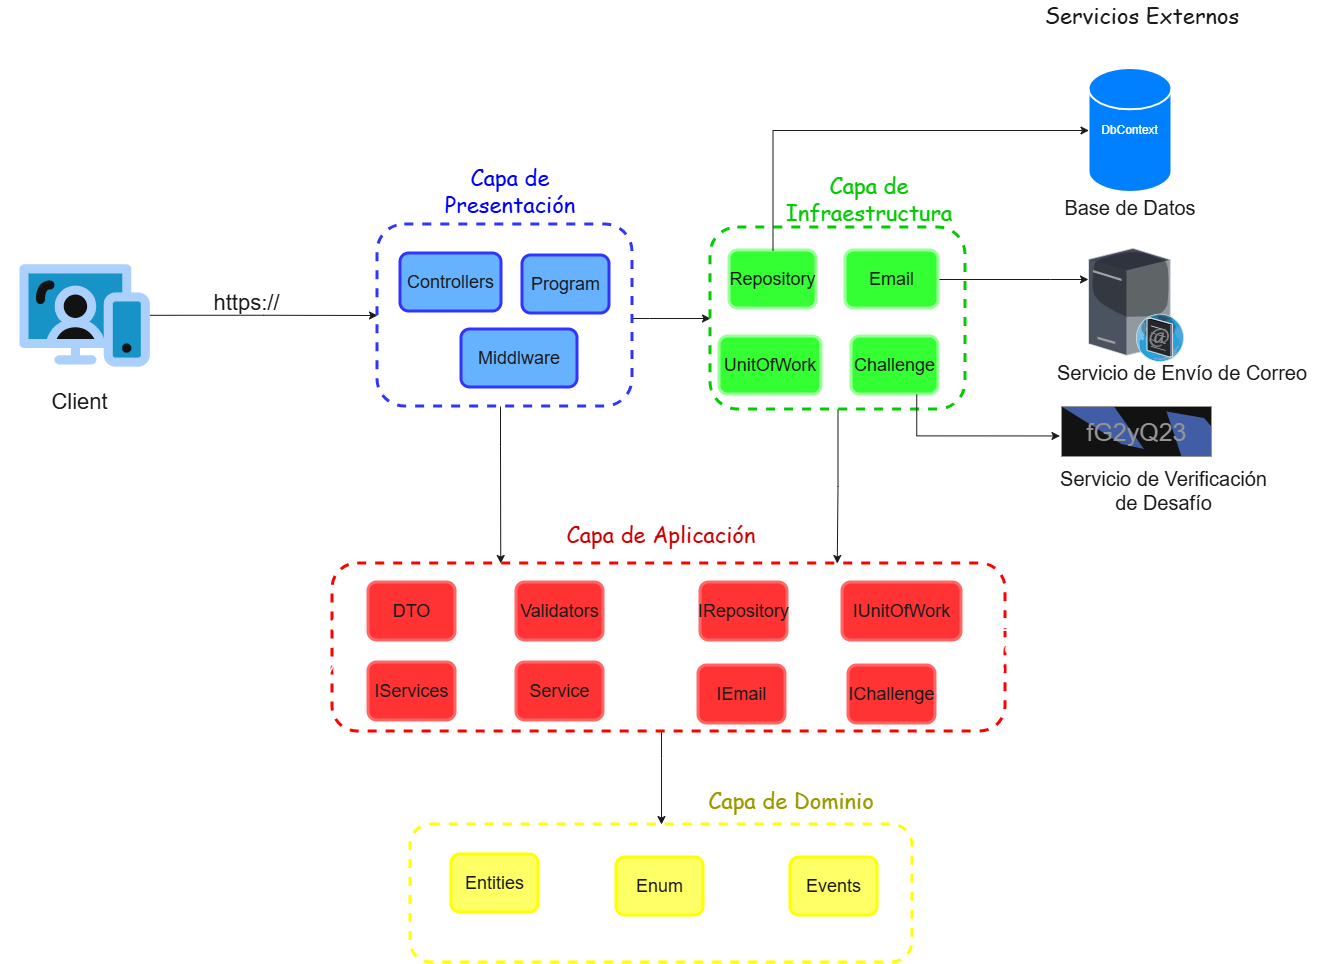
\includegraphics[scale=0.4]{Graphics/Cap3/arquitectura2.drawio.png}
    \caption[Diagrama de la organización del sistema bajo arquitectura limpia]{Diagrama representativo de la organización del sistema bajo un modelo de arquitectura limpia. Fuente: elaboración propia.}
    \label{fig:arquitectura}
\end{figure}

\begin{itemize}
    \item \textbf{Capa de Dominio:} Proyecto central sin dependencias externas. Contiene las entidades de negocio (\texttt{AefiReport}, \texttt{VaccinatedSubject}, \texttt{Vaccine}, \texttt{AdverseEvent}, \texttt{MedicalReviewer}), enumeraciones para clasificación de severidad, estado del paciente.
    
    \item \textbf{Capa de Aplicación:} Depende exclusivamente del proyecto Domain. Contiene los casos de uso organizados según el patrón CQRS: comandos para operaciones de escritura y consultas para lecturas. Define las interfaces de los repositorios, la unidad de trabajo (\texttt{IUnitOfWork}), el servicio de notificaciones (\texttt{INotificationService}), el servicio de envío de correo (\texttt{IEmailSender}), el servicio de verificación de desafío (\texttt{IChallengeVerifier}) y los DTOs para transferencia de datos. Implementa las validaciones de existencia mediante la consulta a repositorios.
    
    \item \textbf{Capa de Infraestructura:} Depende de los proyectos Application y Domain. Proporciona las implementaciones concretas de las interfaces definidas en Application: repositorios con Entity Framework Core sobre MySQL, la unidad de trabajo mediante \texttt{DbContext.SaveChangesAsync}, el servicio de notificaciones, el servicio de envío de correo y el servicio de verificación de CAPTCHA. Contiene además la configuración de autenticación y autorización mediante JWT.
    
    \item \textbf{Capa de Presentación:} Depende del proyecto Application. Corresponde a la API REST desarrollada con ASP.NET Core. Contiene los controladores que reciben las peticiones HTTP, las traducen a comandos o consultas, y retornan las respuestas adecuadas. Implementa las validaciones de formato mediante Data Annotations en los DTOs de entrada. Incluye también la configuración de CORS, Swagger y el middlewares global de excepciones.

\end{itemize}


\subsection{Patrones de Diseño}

La implementación de la Arquitectura Limpia se complementa con un conjunto de patrones de diseño que refuerzan la separación de responsabilidades y la mantenibilidad del sistema. A continuación se describen los más relevantes y se ilustran con fragmentos de código del proyecto.


\subsubsection{Repository}

El patrón Repository abstrae el acceso a los datos mediante una interfaz que simula una colección en memoria, permitiendo al dominio obtener y almacenar objetos sin conocer los detalles de persistencia \cite{evans2003, fowler2002}.

En el proyecto, cada entidad del dominio cuenta con una interfaz de repositorio definida en la capa de Aplicación. La implementación concreta reside en Infraestructura y utiliza Entity Framework Core sobre MySQL. Así, los casos de uso invocan métodos como \texttt{GetByIdAsync} o \texttt{AddAsync} sin depender del \texttt{DbContext} ni del motor de base de datos.

\subsubsection{Unit of Work}

El patrón Unit of Work mantiene el registro de los cambios realizados sobre un conjunto de objetos durante una transacción de negocio y los persiste de forma atómica \cite{fowler2002}.

En el proyecto se implementa mediante la interfaz \texttt{IUnitOfWork} definida en Aplicación. Su implementación en Infraestructura aprovecha el método \texttt{SaveChangesAsync} del \texttt{DbContext} de Entity Framework Core, que por diseño ya actúa como una unidad de trabajo, garantizando que todas las operaciones pendientes se confirmen o se descarten como un solo bloque.

\subsubsection{Inyección de dependencias}

La inyección de dependencias es un patrón mediante el cual un objeto recibe las dependencias que necesita en lugar de instanciarlas directamente, invirtiendo el control de su creación \cite{fowler2004}.

En el proyecto se utiliza el contenedor nativo de ASP.NET Core. En la capa de Presentación se registran todas las interfaces definidas en Aplicación con sus implementaciones concretas en Infraestructura. De este modo, cuando un caso de uso solicita un \texttt{IAefiReportRepository}, el contenedor resuelve automáticamente la implementación concreta, manteniendo las capas internas desacopladas de las externas.

\subsubsection{Mapper}

El patrón Mapper transfiere datos entre dos objetos independientes sin que ninguno conozca la estructura del otro \cite{fowler2002}.

En el proyecto se emplea para convertir entidades de dominio en DTOs y viceversa. Esto evita exponer las entidades fuera de la capa de Aplicación y mantiene el dominio aislado de los formatos de transporte utilizados por la API REST.

\section{Diseño de base de datos}

\subsection{Modelo Entidad-Relación Extendido (MERX)}
% Aquí presentas el diagrama MERX completo con entidades, atributos, 
% claves primarias/foráneas, cardinalidad y herencia (si aplica).

\subsection{Diccionario de datos}
% Descripción detallada de cada tabla: nombre, atributos, tipo de dato, 
% restricciones, valores por defecto, descripción.

\subsection{Normalización}
% Justificas que el esquema cumple con la 3FN (o la que hayas aplicado), 
% mostrando dependencias funcionales y cómo resolviste posibles anomalías.



% \section{Diseño de la interfaz de usuario (UI/UX)}

% \subsection{Pantallas principales}


% \subsection{Justificación de diseño centrado en el usuario}


% \section{Consideraciones de seguridad y privacidad}

% \subsection{Protección de datos sensibles}

% \subsection{Autenticación y autorización}

% \subsection{Protección contra ataques}

% \subsection{Control anti-bot}

% \section{Alternativas de notificación}




%\chapter{Detalles de Implementación}
\label{chapter:implementation}

\section{Introducción}

Este capítulo describe los principales aspectos relacionados con la implementación del sistema web desarrollado para el autorreporte y la gestión operativa de \gls{esavi}. 
El contenido aborda las tecnologías y herramientas incorporadas durante el desarrollo, la organización estructural de la solución y los mecanismos implementados tanto en el backend como en el frontend.

La implementación materializa las decisiones arquitectónicas definidas en el capítulo anterior mediante una arquitectura modular basada en los principios de Clean Architecture y Domain-Driven Design. 
La solución integra mecanismos de autenticación, comunicación asíncrona, persistencia de datos y validación de información, con el propósito de garantizar escalabilidad, mantenibilidad y seguridad.

Además, el capítulo expone los principales componentes funcionales de la plataforma, incluyendo el registro de reportes de ESAVI, la gestión de revisiones médicas, la asignación de responsables y el sistema de notificaciones. 
Finalmente, el contenido aborda elementos asociados al despliegue y la organización técnica de la aplicación.

\section{Tecnologías y herramientas utilizadas}
\label{section:technologies}

\subsection{Tecnologías del backend}

\textbf{C\# y .NET 8.} El backend se desarrolló en C\# sobre .NET 8, un framework de alto rendimiento que ofrece compilación nativa, inyección de dependencias integrada y un ecosistema maduro de bibliotecas para construir APIs REST. La documentación oficial de Microsoft establece que .NET 8 es la versión LTS (Long Term Support) recomendada para aplicaciones en producción \cite{dotnet8}.

\textbf{Entity Framework Core.} La persistencia de datos emplea Entity Framework Core como ORM (Object-Relational Mapper), que permite trabajar con la base de datos mediante objetos de C\# y expresiones LINQ sin escribir consultas SQL manualmente \cite{microsoft_efcore}.

\subsection{Tecnologías de la interfaz de usuario}

\textbf{React con TypeScript.} La interfaz de usuario se construye como una Single Page Application (SPA) en React, una biblioteca de JavaScript que permite crear interfaces interactivas mediante componentes reutilizables. TypeScript añade tipado estático sobre JavaScript, lo que reduce errores en tiempo de desarrollo y mejora la mantenibilidad del código.

\subsection{Sistema gestor de bases de datos}

\textbf{MySQL.} El sistema utiliza MySQL como motor de base de datos relacional. La documentación oficial de MySQL establece que su arquitectura de almacenamiento basada en tablas y su soporte para claves foráneas e índices lo hacen adecuado para aplicaciones que requieren integridad referencial estricta \cite{mysql_docs}. Esta característica resultó determinante para un dominio como el de farmacovigilancia, donde entidades como reportes, sujetos vacunados, revisores y vacunas deben mantener relaciones consistentes.

\subsection{Herramientas de infraestructura y despliegue}

\textbf{Docker.} La contenedorización de la aplicación empleó \textbf{Docker} para garantizar la consistencia entre los entornos de desarrollo, pruebas y producción. La documentación oficial de Docker establece que los contenedores empaquetan el código junto con todas sus dependencias, lo que asegura que el software funcione de manera uniforme en cualquier infraestructura \cite{docker-overview}. Esta característica elimina el clásico problema de ``en mi máquina funciona'' y facilita la distribución del proyecto.

\textbf{Railway.} El despliegue de la API, la base de datos MySQL y los servicios externos como RabbitMQ recayó en \textbf{Railway}, una plataforma como servicio que permite aprovisionar infraestructura en la nube y conectar el despliegue directamente con un repositorio de GitHub \cite{railway-docs}. Railway gestiona de forma automática las variables de entorno, los volúmenes de datos y la exposición de puertos, y activa una nueva construcción y publicación con cada cambio en la rama principal, lo que reduce significativamente el esfuerzo operativo durante el desarrollo \cite{railway-deployments}.

\textbf{Vercel.} Para el \textit{frontend}, el despliegue recayó en \textbf{Vercel}, una plataforma optimizada para aplicaciones web modernas que ofrece integración continua con repositorios de GitHub y distribución global mediante una red de entrega de contenido \cite{vercel-docs}.

Es importante señalar que tanto Railway como Vercel constituyen soluciones de desarrollo y demostración, adoptadas exclusivamente para facilitar que el equipo de investigadores del Instituto Finlay de Vacunas (IFV) y los tutores del proyecto pudieran observar los avances de forma remota y en tiempo real. La arquitectura del sistema está diseñada para migrar y contenerizar en servidores físicos dedicados del IFV cuando el proyecto transite a la etapa de producción, garantizando así el control institucional sobre los datos y la infraestructura.

\subsection{Herramientas de apoyo al desarrollo}

\textbf{Visual Studio Code.} El desarrollo del proyecto transcurrió en \textbf{Visual Studio Code}, con las extensiones oficiales para C\# y Docker. 
Microsoft recomienda este entorno para el desarrollo en .NET, ya que ofrece una integración completa con el SDK y la CLI de .NET \cite{vscode-dotnet}. 
Dicha integración permite crear, compilar y ejecutar aplicaciones directamente desde el editor, lo que agiliza el flujo de trabajo \cite{vscode-csharp}.

\textbf{Git y GitHub.} El control de versiones recayó con \textbf{Git} y el alojamiento del código en \textbf{GitHub}. 
GitHub proporciona un historial completo de cambios donde es posible consultar qué modificaciones ocurrieron, quién las hizo y por qué \cite{github-commits}. 
Al tratarse de un sistema distribuido, cada copia local del repositorio contiene el historial completo del proyecto, lo que permite recuperar cualquier estado anterior del código sin depender del servidor central \cite{pro-git-distributed}.

\textbf{Swagger (Swashbuckle).} Para documentar y probar la API, el proyecto incorporó \textbf{Swagger} a través de la librería Swashbuckle, que genera automáticamente una interfaz web con todos los endpoints, sus parámetros y permite ejecutar peticiones de prueba directamente desde el navegador \cite{swagger-ui}.



% \section{Estructura general de la solución}
% \label{section:solution_structure}

% \subsection{Organización de proyectos}

% \subsection{Separación por capas y responsabilidades}

% \subsection{Estructura modular del sistema}




\section{Implementación de la arquitectura}
\label{section:backend}

Una vez definida la arquitectura del sistema en la sección \ref{section:arquitectura}, este apartado describe cómo se materializaron las decisiones de diseño en código. 
La implementación sigue la estructura en capas propuesta por la arquitectura limpia: dominio, aplicación, infraestructura y presentación. Por cada capa se presentan los patrones utilizados, las tecnologías que los materializan y los fragmentos de código que ilustran las decisiones más relevantes.

\subsection{Capa de Dominio}

La capa de dominio constituye el núcleo del sistema y no depende de ningún otro proyecto de la solución ni de paquetes externos. 
Contiene las entidades de negocio, los objetos de valor, los enumerados, los eventos de dominio y las reglas intrínsecas del dominio de farmacovigilancia. 
Su independencia garantiza que los cambios en la infraestructura o en la presentación no afecten la lógica central del negocio.

\subsubsection{Entidades y agregados}

El diseño de las entidades parte del modelo de base de datos definido en el Capítulo 3. Cada tabla se modela como una clase de C\# que hereda de una jerarquía de clases base diseñada para unificar propiedades comunes y permitir la creación de interfaces genéricas en la capa de aplicación.

La jerarquía de herencia parte de \texttt{BasicEntity}, una clase abstracta que define las marcas de tiempo comunes a todas las entidades del sistema:

\begin{lstlisting}[language={[Sharp]C}, caption={Clase base BasicEntity con marcas de tiempo}, label={lst:basicentity}]
public abstract class BasicEntity
{
    public DateTime CreatedAt { get; set; }
    public DateTime UpdatedAt { get; set; }
}
\end{lstlisting}

Para contemplar entidades con distintos tipos de identificador, el dominio define la interfaz genérica \texttt{IEntity<TId>}:

\begin{lstlisting}[language={[Sharp]C}, caption={Interfaz genérica para identificadores de entidad}, label={lst:ientity}]
public interface IEntity<TId>
{
    TId Id { get; init; }
}
\end{lstlisting}

A partir de esta interfaz, el dominio proporciona dos clases abstractas especializadas. La clase \texttt{GuidEntity} constituye la norma para la mayoría de las entidades del sistema y utiliza un \texttt{Guid} como identificador:

\begin{lstlisting}[language={[Sharp]C}, caption={Clase GuidEntity para entidades con identificador Guid}, label={lst:guidentity}]
public abstract class GuidEntity : BasicEntity, IEntity<Guid>
{
    public Guid Id { get; init; } = new Guid();
}
\end{lstlisting}

Para entidades de catálogo que requieren un identificador entero —como las listas de provincias y municipios, cuyos registros son pocos, estables y no requieren las propiedades de seguridad de un \texttt{Guid}—, existe la clase \texttt{CatalogEntity}.

\begin{lstlisting}[language={[Sharp]C}, caption={Clase CatalogEntity para entidades con identificador entero}, label={lst:catalogentity}]
public abstract class CatalogEntity : BasicEntity, IEntity<int>
{
    public int Id { get; init; }
}
\end{lstlisting}

La elección de \texttt{Guid} como tipo de identificador para las entidades principales responde a criterios de seguridad y escalabilidad. La documentación oficial de Microsoft establece que un \texttt{Guid} (Globally Unique Identifier) es un número pseudoaleatorio de 128 bits con una probabilidad de colisión tan baja que resulta estadísticamente insignificante \cite{microsoft_guid}. A diferencia de los identificadores enteros autoincrementales, un \texttt{Guid} no revela la cantidad de registros en una tabla y no es predecible, lo que refuerza la seguridad de la aplicación. Esta propiedad permite, por ejemplo, exponer el identificador en una URL sin riesgo de que un usuario malintencionado itere sobre valores consecutivos.

Gracias a que \texttt{BasicEntity} unifica las propiedades comunes \texttt{CreatedAt} y \texttt{UpdatedAt}, la capa de aplicación puede definir interfaces genéricas que operan sobre cualquier entidad del sistema sin necesidad de implementaciones específicas por cada tipo. El siguiente fragmento, extraído de la capa de aplicación, ilustra esta ventaja:

\begin{lstlisting}[language={[Sharp]C}, caption={Interfaz genérica que opera sobre cualquier entidad que herede de BasicEntity}, label={lst:genericinterface}]
public interface IGenericRepository<T> where T : BasicEntity
{
    Task<T> GetByIdAsync<TId>(TId elementId);
    Task DeleteByIdAsync<TId>(TId elementId);
}
\end{lstlisting}

La restricción \texttt{where T : BasicEntity} garantiza en tiempo de compilación que la interfaz solo reciba entidades que posean las marcas de tiempo \texttt{CreatedAt} y \texttt{UpdatedAt}, independientemente del tipo de su identificador. Así, el sistema puede incorporar nuevas entidades —ya sea con \texttt{Guid} o con \texttt{int} como identificador— sin modificar las interfaces genéricas existentes, en cumplimiento del Principio de Abierto/Cerrado de \texttt{SOLID}.



\paragraph{Entidades User y Role}

Para la gestión de usuarios y roles, el proyecto emplea las clases \texttt{IdentityUser} y \texttt{IdentityRole} del paquete \texttt{Microsoft.AspNetCore.Identity}. Esta decisión evita implementar desde cero funcionalidades críticas como el almacenamiento seguro de contraseñas, la generación de tokens de verificación y el bloqueo de cuentas tras intentos fallidos.

La entidad \texttt{User} hereda de \texttt{IdentityUser<Guid>} y extiende el modelo con los campos requeridos por el dominio:

\begin{lstlisting}[language={[Sharp]C}, caption={Entidad User que hereda de IdentityUser<Guid>}, label={lst:user}]
public class User : IdentityUser<Guid>
{
    public Guid RoleId { get; set; }
    public DateTime CreatedAt { get; set; }
    public DateTime UpdatedAt { get; set; }
}
\end{lstlisting}

Aunque la clase derivada solo declara tres propiedades adicionales, la herencia de \texttt{IdentityUser<Guid>} aporta un conjunto completo de campos que cubren todas las necesidades de gestión de identidad \cite{microsoft_identity_model}. \texttt{UserName} almacena el nombre de usuario único para el inicio de sesión. \texttt{Email} contiene el correo electrónico empleado para notificaciones y verificación de cuenta. \texttt{PasswordHash} guarda el resultado del algoritmo de hashing y nunca contiene la contraseña en texto plano. \texttt{PhoneNumber} registra el teléfono para autenticación de dos factores o recuperación de cuenta. \texttt{EmailConfirmed} indica si el usuario verificó su correo electrónico. \texttt{LockoutEnd} establece la fecha y hora hasta la cual la cuenta permanece bloqueada tras superar el máximo de intentos fallidos. \texttt{AccessFailedCount} lleva el contador de intentos fallidos consecutivos. \texttt{SecurityStamp} almacena un valor aleatorio que cambia al modificar credenciales, lo que invalida automáticamente sesiones y tokens anteriores.

La entidad \texttt{Role} hereda de \texttt{IdentityRole<Guid>} y mantiene la misma coherencia en el tipo de identificador:

\begin{lstlisting}[language={[Sharp]C}, caption={Entidad Role que hereda de IdentityRole<Guid>}, label={lst:role}]
public class Role : IdentityRole<Guid>{ }
\end{lstlisting}

La herencia de \texttt{IdentityRole<Guid>} proporciona las propiedades \texttt{Name} (nombre único del rol) y \texttt{NormalizedName} (versión normalizada para búsquedas). 
La relación entre usuarios y roles sigue una restricción de uno a muchos: cada usuario posee un único rol mediante la clave foránea \texttt{RoleId} en la entidad \texttt{User}, mientras que un mismo rol puede agrupar a múltiples usuarios. 
Esta decisión simplifica la administración de permisos y refleja los perfiles definidos en el diseño del sistema (administrador, médico evaluador y jefe de vacunación municipal).


El uso de \texttt{Guid} como tipo de identificador en \texttt{IdentityUser} y \texttt{IdentityRole} mantiene la coherencia con la clase \texttt{GuidEntity} definida para el resto de las entidades del sistema, lo que permite que las tablas de identidad compartan el mismo tipo de clave primaria que las tablas de negocio.


\paragraph{Mecanismo de hashing de contraseñas}

La documentación oficial de Microsoft describe que el \texttt{PasswordHasher} de Identity implementa el algoritmo PBKDF2 (Password-Based Key Derivation Function 2), estándar del RFC 2898 que deriva una clave segura a partir de una contraseña \cite{rfc2898}. 
El algoritmo toma la contraseña del usuario, la combina con un \textit{salt} criptográficamente aleatorio de 128 bits y aplica repetidamente la función HMAC-SHA256\footnote{HMAC-SHA256: código de autenticación de mensajes basado en hash \cite{rfc2104}. Funciona aplicando de forma anidada el algoritmo SHA-256 a la combinación de una clave secreta (o \textit{salt}) con el mensaje. Internamente, la clave se procesa mediante una operación XOR con una secuencia de relleno interna (\textit{ipad}) antes de aplicar el primer hash al mensaje; posteriormente, el resultado se combina mediante XOR con una secuencia externa (\textit{opad}) y se somete a un segundo hash SHA-256, garantizando simultáneamente la integridad y autenticidad del resultado.}
durante 100,000 iteraciones como valor predeterminado \cite{microsoft_password_hasher}. Cada iteración adicional duplica el costo computacional de un ataque por fuerza bruta sin afectar perceptiblemente el tiempo de verificación para un usuario legítimo. El formato del hash generado produce una cadena con la siguiente estructura \cite{microsoft_hash_format}:

\begin{center}
\texttt{Base64(salt).Base64(subkey)}
\end{center}

Donde el \textit{salt} es un valor aleatorio único por cada contraseña y el \textit{subkey} es el resultado de aplicar PBKDF2 durante el número configurado de iteraciones.

Este mecanismo garantiza tres propiedades de seguridad esenciales:

\begin{itemize}
    \item \textbf{Unicidad del hash:} dos usuarios con la misma contraseña producen hashes completamente diferentes porque el \textit{salt} generado para cada uno es distinto. Esto impide que un atacante compare hashes para identificar contraseñas idénticas dentro de una base de datos comprometida \cite{owasp_password_storage}.
    
    \item \textbf{Irreversibilidad computacional:} PBKDF2 es una función unidireccional. El elevado número de iteraciones convierte el cálculo del hash en un proceso deliberadamente costoso en tiempo de CPU, lo que ralentiza significativamente cualquier intento de ataque por fuerza bruta incluso si el atacante posee hardware especializado \cite{microsoft_password_hasher}.
    
    \item \textbf{Invalidación de sesiones previas:} la propiedad \texttt{SecurityStamp}, generada aleatoriamente y modificada cada vez que el usuario cambia su contraseña, se incluye en la generación de tokens de autenticación. Si un atacante obtiene credenciales antiguas, el cambio de \texttt{SecurityStamp} invalida inmediatamente cualquier sesión o token previo \cite{microsoft_security_stamp}.
\end{itemize}

La verificación de la contraseña durante el inicio de sesión se realiza internamente mediante el método \texttt{VerifyHashedPassword}, que recalcula el hash con el \textit{salt} almacenado y compara los resultados en tiempo constante, sin que la aplicación necesite conocer el texto plano de la contraseña en ningún momento \cite{microsoft_password_hasher}.





\paragraph{Generación de tokens para verificación de identidad}

El paquete Identity incluye proveedores de tokens integrados que generan cadenas criptográficamente seguras para distintos propósitos. 
El sistema emplea estos tokens durante el proceso de registro para verificar que un usuario controla la dirección de correo electrónico declarada y para permitir el establecimiento seguro de su contraseña inicial. 
La documentación oficial explica que el proveedor predeterminado \texttt{DataProtectorTokenProvider} utiliza internamente la API de Protección de Datos de ASP.NET Core, la cual aplica cifrado autenticado (AES-256-CBC\footnote{AES-256-CBC (Advanced Encryption Standard con modo Cipher Block Chaining y clave de 256 bits): algoritmo de cifrado simétrico estandarizado por el Instituto Nacional de Estándares y Tecnología (NIST, por sus siglas en inglés), agencia del gobierno de Estados Unidos. Transforma datos legibles en texto cifrado usando una clave secreta, y el modo CBC garantiza que mensajes idénticos produzcan resultados cifrados diferentes \cite{nist_aes}.} con HMAC-SHA256) sobre los datos del token \cite{microsoft_token_providers}. 
Esto garantiza tres propiedades de seguridad esenciales: el token no revela información del usuario si es interceptado, cualquier modificación invalida la firma y provoca el rechazo del servidor, y un atacante no puede generar un token válido sin acceder a las claves de protección del servidor \cite{microsoft_data_protection}.

El token posee una vigencia predeterminada de 24 horas, controlada por la propiedad \texttt{TokenLifespan} de \texttt{DataProtectionTokenProviderOptions}, transcurrida la cual expira automáticamente \cite{microsoft_identity_config}. 
La validación ocurre en el servidor sin necesidad de consultar una tabla de tokens pendientes, lo que simplifica la arquitectura y elimina la necesidad de limpiar tokens expirados. 
El caso de uso concreto que orquesta la generación y validación de estos tokens durante el registro de médicos evaluadores se detalla en la sección dedicada a la capa de aplicación.

\paragraph{Configuración de seguridad adicional}

Además de los valores predeterminados, el proyecto configura el número de iteraciones del algoritmo PBKDF2 a 600,000 mediante la clase \texttt{PasswordHasherOptions}:

\begin{lstlisting}[language={[Sharp]C}, caption={Configuración de iteraciones de hashing en Program.cs}, label={lst:passwordoptions}]
builder.Services.Configure<PasswordHasherOptions>(options =>
{
    options.IterationCount = 600_000;
});
\end{lstlisting}

Este ajuste sigue las recomendaciones actuales de OWASP para el algoritmo PBKDF2-SHA256, que establecen un mínimo de 600,000 iteraciones para aplicaciones desplegadas en entornos de producción \cite{owasp_password_storage}. El incremento respecto al valor predeterminado de 100,000 iteraciones aumenta el costo computacional de cada intento de verificación de contraseña en un factor de seis, lo que dificulta aún más los ataques de diccionario sin afectar perceptiblemente el tiempo de inicio de sesión de un usuario legítimo.



\subsubsection{Objetos de valor}

El dominio incluye el objeto de valor \texttt{IdentityNumber}, que encapsula la validación del formato del carné de identidad cubano, la extracción de la fecha de nacimiento y el cálculo de la edad. Esta decisión responde a que varias entidades del sistema —\texttt{VaccinatedSubject}, \texttt{Reporter} y \texttt{MedicalReviewer}— contienen un carné de identidad y requieren las mismas operaciones sobre él. Al extraer esta lógica en un objeto de valor inmutable, se evita la duplicación de código y se garantiza que cualquier validación o cálculo sobre el carné se aplique de manera uniforme en todo el sistema.

\subsubsection{Enumerados}

Los enumerados representan clasificaciones propias del negocio cuyos valores no cambian durante la ejecución de la aplicación. El dominio los define mediante el tipo \texttt{enum} de C\#, lo que garantiza que toda la aplicación comparta las mismas categorías sin riesgo de discrepancias entre capas. Estos tipos no constituyen entidades ni tablas en la base de datos porque sus valores son fijos y no requieren persistencia independiente.

En contraste, conceptos como \texttt{Province} y \texttt{Municipality} sí se modelan como entidades y tablas. Existe una relación entre ambos —cada municipio pertenece a una provincia— que resulta más clara de expresar mediante llaves foráneas que mediante un enumerado extenso. Además, el sistema realiza operaciones frecuentes de búsqueda y filtrado sobre estos datos, para las cuales una tabla indexada ofrece mejor rendimiento. Por último, la lista de provincias y municipios puede actualizarse ocasionalmente por cambios administrativos, y una tabla permite modificarla sin recompilar la aplicación.


\subsubsection{Eventos de dominio}

Los eventos de dominio representan sucesos relevantes del negocio que otras partes del sistema deben conocer. El proyecto los define como clases simples con propiedades que identifican los datos del suceso y los utiliza para desencadenar el envío de notificaciones por correo electrónico sin acoplar la lógica de envío a las entidades. Esta arquitectura mantiene el dominio aislado de los detalles de infraestructura y permite agregar nuevos manejadores sin modificar las entidades ni los casos de uso.

Durante la implementación surgieron además dos entidades de infraestructura no previstas en el diseño inicial: \texttt{RefreshToken}, que permite la renovación de sesiones sin reautenticación, y \texttt{AuditLog}, que registra las operaciones realizadas sobre el sistema con fines de trazabilidad. Ambas heredan de \texttt{GuidEntity} y su definición detallada se presenta en el Anexo \ref{anexo:entidades_infraestructura}.



\subsection{Capa de Aplicación}
\label{subsection:aplicacion}

La capa de aplicación orquesta los casos de uso del sistema. Recibe comandos y consultas desde la capa de presentación, coordina las entidades del dominio y los servicios de infraestructura, y retorna resultados transformados en DTOs. Esta capa depende exclusivamente del dominio, por lo que desconoce los detalles de la base de datos, el envío de correos o la generación de tokens.

\subsubsection{Casos de uso y servicios de aplicación}

Los casos de uso se implementan mediante servicios de aplicación que el controlador invoca a través de interfaces. Esta decisión responde al patrón de Inyección de Dependencias (Dependency Injection, DI): en lugar de que cada clase cree sus propias dependencias mediante \texttt{new}, el contenedor de DI de ASP.NET Core las suministra automáticamente al constructor. 
El desarrollador registra qué implementación concreta corresponde a cada interfaz, y el contenedor resuelve las dependencias en tiempo de ejecución \cite{ms_di_doc}.

Este patrón resuelve un problema concreto de acoplamiento. Sin DI, la capa de presentación necesitaría conocer las clases concretas de la capa de aplicación para instanciarlas. Con DI, la presentación solo declara la interfaz en su constructor, sin saber qué implementación recibe ni dónde se encuentra. 
Así, si la lógica de negocio cambia, solo debe modificarse la capa de aplicación; la presentación permanece intacta. Este mismo principio se aplica en todas las capas del sistema: la capa de aplicación declara interfaces de repositorio que la infraestructura implementa, y la capa de infraestructura declara interfaces de servicios externos que los proveedores concretos satisfacen. 
El contenedor centraliza las dependencias en métodos como \texttt{AddAplication} e \texttt{AddInfrastructure}:

\begin{lstlisting}[language={[Sharp]C}, caption={Registro de servicios en el contenedor de DI}, label={lst:di_registration}]
// Capa de aplicación: AddAplication
services.AddScoped<IReportCommandService, ReportCommandService>();
services.AddScoped<IReportQueryService, ReportQueryService>();
services.AddScoped<IIdentityService, IdentityService>();

// Capa de infraestructura: AddInfrastructure
services.AddScoped<IUnitOfWork, UnitOfWork>();
services.AddScoped<IJwtTokenGenerator, JwtTokenGenerator>();
services.AddScoped<IEmailService, EmailJsService>();
\end{lstlisting}

El siguiente fragmento muestra cómo el controlador recibe \texttt{IIdentityService} sin conocer su implementación, y cómo el servicio de aplicación recibe a su vez \texttt{IJwtTokenGenerator} y \texttt{IUnitOfWork} bajo el mismo principio:

\begin{lstlisting}[language={[Sharp]C}, caption={Inyección de abstracciones en todas las capas}, label={lst:di_controller}]
// Capa de presentación: solo conoce la interfaz
public class AuthenticationController : ControllerBase
{
    private readonly IIdentityService _identityService;

    public AuthenticationController(IIdentityService identityService)
    {
        _identityService = identityService;
    }
}

// Capa de aplicación: recibe interfaces, no implementaciones
public class IdentityService : IIdentityService
{
    private readonly IJwtTokenGenerator _jwtTokenGenerator;
    private readonly IUnitOfWork _unitOfWork;

    public IdentityService(
        IJwtTokenGenerator jwtTokenGenerator,
        IUnitOfWork unitOfWork)
    {
        _jwtTokenGenerator = jwtTokenGenerator;
        _unitOfWork = unitOfWork;
    }
}
\end{lstlisting}

El sistema aplica además el Principio de Separación de Comandos y Consultas (CQS), propuesto por Bertrand Meyer, que establece que una operación debe ser un comando —modifica el estado sin retornar datos— o una consulta —retorna datos sin modificar el estado—, pero nunca ambas cosas \cite{Meyer1988}. 
Llevado a la arquitectura, cada recurso del dominio define dos interfaces: una para comandos y otra para consultas. 
El siguiente fragmento muestra esta separación para el recurso de reportes:

\begin{lstlisting}[language={[Sharp]C}, caption={Separación CQS en interfaces de reportes}, label={lst:cqs}]
// Comandos: modifican el estado
public interface IReportCommandService
{
    Task<Guid> CreatePublicReportAsync(PublicAefiReportDto dto);
    Task CompleteReviewAsync(CompleteReviewDto dto);
}

// Consultas: retornan datos sin modificar
public interface IReportQueryService
{
    Task<PagedResultDto<ReportDto>> GetReportsAsync(PagedRequestDto paged);
    Task<ReportDto> GetReportByNotificationNumber(string notificationNumber);
}
\end{lstlisting}

Esta separación no alcanza la complejidad de un CQRS completo —ambos servicios comparten el mismo modelo de dominio y la misma base de datos—, pero permite que cada interfaz evolucione según sus necesidades específicas.

Los servicios de aplicación coordinan los repositorios y el Unit of Work para ejecutar los casos de uso. El siguiente fragmento, extraído de \texttt{IdentityService}, muestra cómo un caso de uso orquesta múltiples dependencias dentro de una misma transacción:

\begin{lstlisting}[language={[Sharp]C}, caption={Orquestación de dependencias en un caso de uso}, label={lst:orchestration}]
public async Task<UserResponseDTO> LoginUserAsync(LoginUserDto loginDto)
{
    var savedUser = await _identityManager.CheckCredentialsAsync(
        loginDto.Email, loginDto.Password)
        ?? throw new ArgumentException("Invalid credentials");

    var accessToken = await _jwtTokenGenerator.GenerateToken(savedUser);
    var refreshToken = GenerateRefreshToken();

    await _unitOfWork.GetRepository<RefreshToken>().CreateAsync(
        new RefreshToken
        {
            Token = refreshToken,
            ExpiresAt = DateTime.UtcNow.AddDays(7),
            UserId = savedUser.Id
        });

    await _unitOfWork.CompleteAsync();

    return new UserResponseDTO { ... };
}
\end{lstlisting}

\subsubsection{Mapeo y transformación de datos}

La capa de aplicación define DTOs (Data Transfer Objects, objetos de transferencia de datos) para mover información entre la API y el dominio. Un DTO es un objeto plano que contiene solo propiedades, sin lógica de negocio, diseñado para transportar datos en un formato adecuado para el cliente. Las entidades del dominio no se exponen fuera de esta capa, lo que protege al núcleo del sistema de cambios en los formatos de intercambio y evita la exposición accidental de propiedades internas.

El sistema emplea AutoMapper para convertir entidades en DTOs y viceversa, aplicando el patrón Mapper \cite{fowler_mapper}. 
AutoMapper permite definir reglas de transformación en clases llamadas perfiles, que heredan de \texttt{Profile} y centralizan las conversiones entre tipos. 
Cada perfil declara cómo se asigna cada propiedad de un tipo origen a un tipo destino, incluyendo propiedades anidadas que requieren lógica adicional:

\begin{lstlisting}[language={[Sharp]C}, caption={Perfil de mapeo con AutoMapper}, label={lst:mapper_profile}]
public class AefiReportProfile : Profile
{
    public AefiReportProfile()
    {
        CreateMap<AefiReport, ReportDto>()
            .ForMember(dest => dest.SubjectName,
                opt => opt.MapFrom(src => src.VaccinatedSubject.FullName))
            .ForMember(dest => dest.VaccineNames,
                opt => opt.MapFrom(src => src.Vaccinations
                    .Select(v => v.Lot.Vaccine.Name)));
    }
}
\end{lstlisting}

En este ejemplo, \texttt{SubjectName} no existe directamente en \texttt{AefiReport}, sino que se obtiene navegando la relación hacia \texttt{VaccinatedSubject}. 
AutoMapper resuelve esta navegación automáticamente y genera la consulta SQL correspondiente.

Para las consultas, el sistema aprovecha el método \texttt{ProjectTo<T>} de AutoMapper. 
A diferencia de un mapeo en memoria —que cargaría la entidad completa para luego transformarla—, \texttt{ProjectTo} traduce la proyección directamente a SQL, de modo que solo las columnas necesarias viajan desde la base de datos hasta la aplicación:

\begin{lstlisting}[language={[Sharp]C}, caption={Proyección directa a DTO con ProjectTo}, label={lst:projectto}]
var items = await _unitOfWork.GetRepository<AefiReport>()
    .GetPaged(query, skip, take)
    .ProjectTo<ReportDto>(_mapper.ConfigurationProvider)
    .ToListAsync();
\end{lstlisting}

Esta técnica mejora el rendimiento de las consultas al evitar la carga completa de las entidades y sus relaciones, y al delegar la selección de columnas al motor de base de datos.


\subsubsection{Validaciones y manejo de solicitudes}

El sistema aplica dos niveles de validación sobre cada solicitud entrante, en momentos distintos del procesamiento y con propósitos complementarios.

El primer nivel opera sobre los DTOs mediante atributos de validación de .NET. 
Estos atributos verifican condiciones simples —obligatoriedad, longitud máxima, formato de correo electrónico o número de teléfono— antes de que la solicitud alcance el servicio de aplicación. ASP.NET Core ejecuta esta validación automáticamente al construir el DTO desde el cuerpo de la solicitud, gracias al atributo \texttt{[ApiController]}. 
Si algún atributo falla, el middleware devuelve un código 400 con los campos que incumplieron la validación. El siguiente fragmento muestra un DTO con atributos de validación estándar y personalizados:

\begin{lstlisting}[language={[Sharp]C}, caption={DTO con atributos de validación}, label={lst:dto_validation}]
public class VaccinatedSubjectDto
{
    [Required(ErrorMessage = "Full name is required.")]
    [StringLength(150, MinimumLength = 1)]
    public string FullName { get; set; } = string.Empty;

    [Required(ErrorMessage = "Identity number is required.")]
    [IdentityNumberValidation]
    public string IdentityNumber { get; set; } = string.Empty;
    
    // el resto de atributos
}
\end{lstlisting}

Los atributos personalizados \texttt{IdentityNumberValidation} y \texttt{EmailValidation}, definidos en la capa de aplicación, heredan de \texttt{ValidationAttribute} y encapsulan reglas reutilizables sin duplicar código en múltiples DTOs:

\begin{lstlisting}[language={[Sharp]C}, caption={Atributo de validación personalizado}, label={lst:custom_validation}]
public class IdentityNumberValidationAttribute : ValidationAttribute
{
    protected override ValidationResult? IsValid(object? value,
        ValidationContext validationContext)
    {
        // valida que tenga formato de 11 dígitos y coherencia
        return ValidationResult.Success;
    }
}
\end{lstlisting}

El segundo nivel opera dentro del servicio de aplicación, una vez que la solicitud superó las validaciones de formato. Este nivel aplica reglas de negocio que requieren consultar la base de datos o comparar datos de múltiples fuentes: verificar que una vacuna exista, que un lote pertenezca a la vacuna declarada, o que la fecha de administración de la vacuna no sea posterior a la fecha de inicio de los síntomas. Para ello, el sistema define la interfaz \texttt{IReportValidator<T>} y la inyecta en los servicios de aplicación mediante el contenedor de dependencias:

\begin{lstlisting}[language={[Sharp]C}, caption={Inyección de validadores en el servicio de aplicación}, label={lst:validator_injection}]
public class ReportCommandService : IReportCommandService
{
   // constructor de la clase y variables privadas
   
    public async Task<CreateReportResponseDto> CreatePublicReportAsync(
        PublicAefiReportDto reportDto)
    {
        // Ejecuta todos los validadores registrados para este tipo de DTO
        foreach (var validator in _validators)
            await validator.ValidateAsync(reportDto);

        // Continúa con la creación del reporte...
    }
}
\end{lstlisting}

El contenedor de dependencias resuelve automáticamente todas las implementaciones de \texttt{IReportValidator<T>} registradas y las inyecta como una colección. Esto permite que el servicio ejecute todos los validadores sin conocer sus tipos concretos, en cumplimiento del Principio de Abierto/Cerrado: agregar una nueva regla de validación solo requiere implementar la interfaz y registrarla en el contenedor, sin modificar el servicio de aplicación.

Este mismo patrón de validación en segundo nivel aplica a otras reglas de negocio que operan sobre datos ya persistidos. 
Un ejemplo es la expiración de asignaciones, implementada en \texttt{IAssignmentExpirationService}. 
Esta regla materializa RN-07 y RN-08 (Capítulo \ref{chapter:proposal}): determina la prioridad del reporte a partir del evento adverso más grave que contenga y aplica el plazo de evaluación correspondiente —24 horas para prioridad alta, 5 días para prioridad media y 7 días para prioridad baja—. 
El servicio consulta las asignaciones pendientes, compara su fecha de asignación con el plazo según la prioridad del reporte asociado y marca como expiradas aquellas que lo superan.

La capa de aplicación extiende el principio de inversión de dependencias a los servicios de infraestructura que necesita para completar sus casos de uso.
Para acceder a los datos, la aplicación declara interfaces de repositorio como \texttt{IGenericRepository<T>} y \texttt{IUserRepository}, cuyas implementaciones residen en la capa de infraestructura. Para enviar notificaciones, declara \texttt{IEmailService} sin saber si el envío utiliza un servicio externo, un servidor SMTP o cualquier otro mecanismo. Para la autenticación, declara \texttt{IJwtTokenGenerator} e \texttt{IIdentityManager} sin conocer los algoritmos de firma ni las claves secretas. 
En cada caso, el servicio de aplicación solo conoce la interfaz y confía en que el contenedor de DI suministrará la implementación registrada en \texttt{AddInfrastructure}. Esta separación permite cambiar el proveedor de correo electrónico, el motor de base de datos o el servicio de CAPTCHA sin modificar una sola línea de la capa de aplicación.







\subsection{Capa de Infraestructura}

La capa de infraestructura implementa los contratos definidos en las capas de dominio y aplicación. Contiene el acceso a la base de datos, la generación de tokens, el envío de correos electrónicos, la mensajería asíncrona y la integración con servicios externos. Todas las dependencias hacia el mundo exterior residen aquí, lo que permite que el núcleo del sistema permanezca independiente de tecnologías concretas.


\subsubsection{Persistencia de datos y configuración de Entity Framework Core}

El sistema utiliza MySQL como motor de base de datos relacional. 
La conexión se establece mediante una cadena de conexión —que contiene el servidor, el nombre de la base de datos y las credenciales de acceso— almacenada en las variables de entorno del servidor bajo el nombre \texttt{AppDbConnectionString}. 
El paquete Pomelo.EntityFrameworkCore.MySql, un proveedor de .NET que adapta Entity Framework Core a las características específicas de MySQL \cite{mysql_efcore}, toma esta cadena y la utiliza para establecer la comunicación con la base de datos. 
La configuración se realiza durante el arranque de la aplicación, en un método de extensión llamado \texttt{AddInfrastructure} que centraliza el registro de todos los servicios de esta capa en el contenedor de inyección de dependencias:

\begin{lstlisting}[language={[Sharp]C}, caption={Configuración de la conexión a MySQL}, label={lst:mysqlconfig}]
var connectionString = configuration.GetConnectionString("AppDbConnectionString");
services.AddDbContext<FinlayDbContext>(options =>
    options.UseMySql(connectionString, ServerVersion.AutoDetect(connectionString)));
\end{lstlisting}

Sobre esta conexión, el contexto \texttt{FinlayDbContext} —la clase que representa la sesión con la base de datos— centraliza el acceso a todas las tablas del sistema. 
Las características de infraestructura de cada tabla se definen en el método \texttt{OnModelCreating} mediante la API fluida de Entity Framework Core, sin decorar las clases del dominio con atributos propios de la persistencia \cite{microsoft_efcore}. 
Este método aplica las mismas restricciones definidas en el diseño de la base de datos (Capítulo 3, Sección 3.5): nulabilidad, longitudes máximas, llaves foráneas e índices\footnote{Un índice es una estructura de datos que permite al motor de base de datos localizar filas sin recorrer toda la tabla, de forma similar al índice alfabético de un libro. El sistema define índices sobre columnas consultadas con frecuencia.}.
Además, cada relación declara un comportamiento de borrado y actualización: \texttt{Cascade} propaga la operación cuando la entidad dependiente carece de sentido sin su principal, mientras que \texttt{Restrict} la bloquea si existen registros referenciados desde otra tabla. 
El siguiente fragmento, correspondiente a la entidad \texttt{AefiReport}, ilustra estas decisiones:

\begin{lstlisting}[language={[Sharp]C}, caption={Configuración de infraestructura para AefiReport}, label={lst:fluentapi}]
builder.Entity<AefiReport>(entity =>
{
    entity.HasKey(e => e.Id);
    entity.Property(e => e.NotificationNumber)
          .IsRequired()
          .HasMaxLength(100);
    entity.HasIndex(e => e.NotificationNumber).IsUnique();
    entity.HasOne(r => r.VaccinatedSubject)
          .WithMany(p => p.AefiReports)
          .HasForeignKey(r => r.VaccinatedSubjectId)
          .OnDelete(DeleteBehavior.Restrict);

    // otros atributos y llaves foráneas
});
\end{lstlisting}


\subsubsection{Migraciones y acceso a datos}

El acceso a los datos se implementa mediante el patrón Repository, que abstrae las operaciones de persistencia detrás de interfaces definidas en la capa de aplicación. La clase \texttt{GenericRepository<T>} proporciona una implementación genérica para operaciones comunes —crear, obtener por identificador, listar, actualizar y eliminar— y aprovecha la restricción \texttt{where T : BasicEntity} para operar sobre cualquier entidad del sistema sin duplicar código:

\begin{lstlisting}[language={[Sharp]C}, caption={Repositorio genérico}, label={lst:genericrepository}]
public class GenericRepository<T> : IGenericRepository<T> where T : BasicEntity
{
    protected readonly DbSet<T> _entity;

    public virtual async Task<T> CreateAsync(T element) { ... }
    public virtual async Task<T> GetByIdAsync<TId>(TId elementId) { ... }
    public virtual IQueryable<T> GetAll() { ... }
    public virtual void Update(T element) { ... }
    public virtual async Task DeleteByIdAsync<TId>(TId elementId) { ... }
}
\end{lstlisting}

Cuando una entidad requiere consultas que el repositorio genérico no cubre, el sistema define repositorios especializados que heredan de \texttt{GenericRepository<T>} y añaden métodos particulares. Todas las consultas utilizan LINQ, el lenguaje de consulta integrado de C\#, que Entity Framework Core traduce automáticamente a SQL. El siguiente ejemplo muestra una consulta LINQ y la sentencia SQL equivalente que se ejecuta en la base de datos:

\begin{lstlisting}[language={[Sharp]C}, caption={Consulta LINQ y su traducción a SQL}, label={lst:linq}]
// LINQ
var reportes = await _entity
    .Where(r => r.Status == AefiReportStatus.UnderReview)
    .OrderByDescending(r => r.ReportDate)
    .Take(10)
    .ToListAsync();

// SQL generado
SELECT TOP 10 *
FROM AefiReports
WHERE Status = 'UnderReview'
ORDER BY ReportDate DESC;
\end{lstlisting}

El patrón Unit of Work, implementado en la clase \texttt{UnitOfWork}, coordina las operaciones de múltiples repositorios dentro de una única transacción. 
Su método \texttt{CompleteAsync} invoca \texttt{SaveChangesAsync} del contexto. 
Esto garantiza que todos los cambios realizados durante un caso de uso se persistan de forma atómica: si cualquier operación falla, ninguna se materializa en la base de datos \cite{martin_fowler_uow}.

El registro de auditoría se implementa mediante un interceptor de Entity Framework Core que hereda de \texttt{SaveChangesInterceptor}. 
Este interceptor se ejecuta automáticamente antes de cada \texttt{SaveChangesAsync}: recorre las entidades modificadas, serializa los valores anteriores y posteriores de cada operación, y añade los registros correspondientes a la tabla \texttt{AuditLog}. 
Como el interceptor opera dentro de la misma transacción, la auditoría y los cambios de negocio se persisten de forma atómica. 
Esta solución mantiene la transparencia para los casos de uso, que no necesitan invocar ningún servicio de auditoría.

\subsubsection{Integración con servicios externos}

El sistema integra cuatro servicios externos principales: 


\textbf{Friendly CAPTCHA\footnote{CAPTCHA (Completely Automated Public Turing test to tell Computers and Humans Apart): prueba de Turing automatizada que distingue a un humano de un ordenador.}.} Los endpoints públicos están expuestos a ataques automatizados que envían solicitudes directamente a la API. Como primera barrera, el sistema utiliza Friendly CAPTCHA, un servicio de verificación basado en prueba de trabajo criptográfica (proof-of-work) que no afecta la experiencia del usuario. La sección de seguridad (Apartado \ref{section:seguridad}) detalla el fundamento y el flujo de verificación de este mecanismo.

\textbf{Notificaciones por correo electrónico y WhatsApp.} El sistema necesita notificar a los usuarios sobre eventos relevantes —confirmación de reporte, asignación a revisor, expiración de asignación— a través de canales accesibles para la población cubana. La vía de SMS resultó inviable para esta etapa por razones de infraestructura y costo, por lo que el sistema adopta el correo electrónico y WhatsApp, las dos vías con mayor penetración en la ciudadanía cubana.

\textbf{EmailJS.} Para el envío de correos electrónicos, el sistema utiliza EmailJS, un servicio que permite enviar correos sin configurar un servidor SMTP propio. 
El servicio \texttt{EmailJsService} implementa la interfaz \texttt{IEmailService} y construye una solicitud HTTP a la API de EmailJS con los parámetros de la plantilla, el identificador del servicio y el token de acceso, todos configurados en \texttt{EmailJsSettings}:

\begin{lstlisting}[language={[Sharp]C}, caption={Envío de correo mediante EmailJS}, label={lst:emailjs}]
var payload = new
{
    service_id = _settings.ServiceId,       
    template_id = templateId,                
    user_id = _settings.UserId,             
    accessToken = _settings.AccessToken,   
    template_params = templateParams          // diccionario que tiene los datos específicos de la plantilla
};

// Serializar y enviar la solicitud a la API de EmailJS
var json = JsonSerializer.Serialize(payload);
var content = new StringContent(json, Encoding.UTF8, "application/json");
var response = await _httpClient.PostAsync(url, content);
\end{lstlisting}

Cada tipo de notificación se corresponde con una plantilla predefinida, identificada por un \texttt{template\_id}. 
Los datos específicos de cada plantilla viajan dentro del objeto \texttt{template\_params}, que el servicio construye dinámicamente a partir de los datos recibidos desde la capa de aplicación.

\textbf{OpenWA (WhatsApp).} Para las notificaciones por WhatsApp, el sistema utiliza OpenWA, una API de código abierto que permite enviar mensajes mediante un servidor intermediario conectado a un número de teléfono registrado. A diferencia de la API oficial de WhatsApp Business de Meta, OpenWA no exige verificación empresarial ni tiene costo por mensaje, lo que la hace adecuada para la etapa de prototipado. El servicio que implementa esta integración sigue el mismo patrón que EmailJS: recibe los datos de la notificación desde la capa de aplicación, los transforma al formato esperado por OpenWA y envía la solicitud HTTP correspondiente. Las credenciales de acceso —URL del servidor y token de autenticación— residen en variables de entorno, sin exponerse en el código fuente.

Tanto EmailJS como OpenWA constituyen soluciones para la etapa de desarrollo y demostración. La arquitectura en capas permite migrar a servicios de producción sin modificar la lógica de negocio: EmailJS puede reemplazarse por un servidor SMTP institucional del IFV o por servicios como SendGrid o Resend con planes extensivos; OpenWA puede migrar a la API oficial de WhatsApp Business de Meta cuando el proyecto transite a producción.

\textbf{Generación de PDF.} El servicio \texttt{PdfService} utiliza la librería QuestPDF para generar documentos PDF a partir de los datos de un reporte ESAVI. QuestPDF emplea una API fluida que describe la estructura del documento —páginas, tablas, texto— en código C\# sin depender de plantillas HTML ni de librerías externas \cite{questpdf}.



\subsubsection{Comunicación asíncrona mediante mensajería}

Cuando un usuario completa un reporte ESAVI, el sistema valida los datos, los persiste y envía una notificación de confirmación por correo electrónico. Aunque la operación principal se procesa correctamente, la notificación depende de un servicio externo sujeto a latencia de red o indisponibilidad temporal. Si el envío se ejecuta dentro del mismo hilo que atiende la solicitud HTTP, el usuario percibe esa demora o nunca recibe la confirmación a pesar de que su reporte se guardó exitosamente.

Las colas de mensajes resuelven este problema desacoplando la operación principal de sus efectos secundarios. El caso de uso deposita un mensaje en la cola y retorna de inmediato al usuario; el mensaje se procesa en segundo plano. Si el procesamiento falla, el mensaje permanece en la cola y puede reintentarse sin afectar al usuario.

El sistema utiliza RabbitMQ como intermediario de mensajería y MassTransit como librería de integración con .NET \cite{masstransit}. Para mantener la capa de aplicación independiente de MassTransit, el sistema define una abstracción propia: la interfaz \texttt{IEventBus}, que expone un único método \texttt{PublishAsync}. La implementación concreta, \texttt{MassTransitEventBus}, reside en la capa de infraestructura y delega en \texttt{IPublishEndpoint} de MassTransit. La configuración se centraliza en el método \texttt{AddInfrastructure}:

\begin{lstlisting}[language={[Sharp]C}, caption={Configuración de MassTransit con RabbitMQ}, label={lst:masstransit}]
services.AddMassTransit(x =>
{
    x.AddConsumer<MedicalReviewerConsumer>();
    x.AddConsumer<AssignmentExpiredConsumer>();
    x.AddConsumer<ReportConfirmationConsumer>();

    x.UsingRabbitMq((context, cfg) =>
    {
        cfg.Host(rabbitMqUrl);
        cfg.ConfigureEndpoints(context);
    });
});

services.AddScoped<IEventBus, MassTransitEventBus>();
\end{lstlisting}

Cada consumidor implementa la interfaz \texttt{IConsumer<T>} de MassTransit, donde \texttt{T} es el tipo de evento de dominio que procesa. El siguiente fragmento muestra el patrón de uso: el caso de uso guarda el reporte, publica el evento a través de \texttt{IEventBus} y retorna al usuario sin esperar:

\begin{lstlisting}[language={[Sharp]C}, caption={Publicación de un evento tras crear un reporte}, label={lst:publishevent}]
await _unitOfWork.GetRepository<AefiReport>().CreateAsync(report);
await _unitOfWork.CompleteAsync();

await _eventBus.PublishAsync(new ReportConfirmationEvent
{
    ReportNumber = report.NotificationNumber,
    Email = reporter.Email,
    SymptomsName = symptomNames,
    VaccinesName = vaccinesNames,
    ReportDate = report.ReportDate
});

return new CreateReportResponseDto
{
    NotificationNumber = report.NotificationNumber
};
\end{lstlisting}

El método \texttt{PublishAsync} envía el evento a RabbitMQ y retorna de inmediato. En segundo plano, \texttt{ReportConfirmationConsumer} recibe el mensaje y ejecuta el envío mediante \texttt{IEmailService}. Si el envío falla, MassTransit aplica reintentos automáticos con intervalos crecientes, sin que el usuario perciba el error. El mismo mecanismo aplica al resto de notificaciones del sistema: asignación de un reporte a un médico revisor, expiración de una asignación no completada, nuevo reporte recibido por un jefe de vacunación municipal y correo de activación de cuenta para un revisor recién registrado.



Para las asignaciones que no se completan en el plazo establecido, un servicio en segundo plano verifica periódicamente las pendientes. 
Este servicio hereda de \texttt{BackgroundService}, clase base de .NET recomendada para tareas de larga duración \cite{microsoft_background}.

\begin{lstlisting}[language={[Sharp]C}, caption={Servicio en segundo plano para expiración de asignaciones}, label={lst:backgroundservice}]
public class AssignmentExpirationBackgroundService : BackgroundService
{
    ...
    protected override async Task ExecuteAsync(CancellationToken stoppingToken)
    {
        while (!stoppingToken.IsCancellationRequested)
        {
            // Crear un ámbito para acceder a servicios scoped
            using var scope = _scopeFactory.CreateScope();
            var service = scope.ServiceProvider
                .GetRequiredService<IAssignmentExpirationService>();

            // Ejecutar la lógica de negocio en capa de aplicación
            await service.ProcessExpiredAssignmentsAsync(stoppingToken);

            // Esperar 3 horas antes de la próxima verificación
            await Task.Delay(TimeSpan.FromHours(3), stoppingToken);
        }
    }
}
\end{lstlisting}

En cada ciclo, el servicio invoca a \texttt{IAssignmentExpirationService}, el servicio de aplicación encargado de localizar las asignaciones pendientes cuyo plazo expiró, marcarlas como expiradas, reabrir los reportes asociados y publicar los eventos correspondientes a través de \texttt{IEventBus}. 
Las reglas de negocio que determinan los plazos de expiración según la severidad del reporte se detallan en la capa de aplicación (Apartado \ref{subsection:aplicacion}). 
Los consumidores reciben estos eventos y envían las notificaciones por correo electrónico al jefe de vacunación municipal correspondiente.







\subsection{Capa de Presentación}

La capa de presentación constituye el punto de entrada al sistema desde el exterior. Materializa los principios de la arquitectura limpia al depender exclusivamente de la capa de aplicación: los controladores reciben solicitudes HTTP, las transforman en comandos o consultas, y retornan respuestas estructuradas sin contener lógica de negocio.

\subsubsection{Diseño de la API REST}

El sistema expone una API REST que sigue las convenciones del protocolo HTTP. Esta decisión responde a dos razones: REST utiliza los verbos y códigos de estado estándar de HTTP, lo que facilita la integración con cualquier frontend web o móvil sin necesidad de librerías propietarias, y su modelo sin estado —cada solicitud contiene toda la información necesaria para procesarla— simplifica el escalamiento horizontal y la depuración \cite{fielding2000}. Cada recurso del dominio —reportes, revisores médicos, asignaciones, vacunas— se identifica mediante una ruta única bajo el prefijo \texttt{/api/}. Los controladores utilizan los verbos HTTP estándar conforme a su propósito: \texttt{POST} para crear recursos, \texttt{GET} para consultarlos, \texttt{PUT} para modificarlos y \texttt{DELETE} para eliminarlos.

Las respuestas siguen una estructura uniforme. Las operaciones exitosas retornan el código HTTP correspondiente junto con un objeto JSON que contiene un mensaje descriptivo y los datos solicitados. El siguiente fragmento, extraído del controlador de reportes, ilustra esta convención:

\begin{lstlisting}[language={[Sharp]C}, caption={Respuesta estructurada en el controlador de reportes}, label={lst:apiresponse}]
return StatusCode(StatusCodes.Status201Created, new
{
    message = "Report successfully created",
    data = result
});
\end{lstlisting}

Los códigos de estado HTTP comunican el resultado de cada operación de forma inequívoca: 201 para creación exitosa, 200 para consultas, 400 para errores de validación, 404 para recursos no encontrados y 500 para errores internos. Cada endpoint declara explícitamente los códigos que puede retornar mediante el atributo \texttt{[ProducesResponseType]}, lo que permite a Swagger documentarlos automáticamente.

\subsubsection{Controladores y endpoints}

Los controladores organizan los endpoints por recurso del dominio y actúan como fachada entre el protocolo HTTP y los casos de uso de la capa de aplicación. El sistema define controladores para autenticación, reportes, revisores médicos, asignaciones, vacunas, síntomas, provincias y centros de vacunación.

Cada controlador recibe mediante inyección de dependencias únicamente los servicios de aplicación que necesita. El controlador de reportes, por ejemplo, depende de \texttt{IReportQueryService} para consultas e \texttt{IReportCommandService} para comandos, lo que materializa el patrón CQRS desde la presentación:

\begin{lstlisting}[language={[Sharp]C}, caption={Controlador de reportes con separación CQRS}, label={lst:reportcontroller}]
[ApiController]
[Route("api/[controller]")]
public class ReportController : ControllerBase
{
    private readonly IReportQueryService _reportQueryService;
    private readonly IReportCommandService _reportCommandService;

    public ReportController(
        IReportQueryService reportQueryService,
        IReportCommandService reportCommandService)
    {
        _reportQueryService = reportQueryService;
        _reportCommandService = reportCommandService;
    }
}
\end{lstlisting}

Los atributos \texttt{[ApiController]} y \texttt{[Route]} configuran el comportamiento del controlador: el primero habilita la validación automática del modelo y la inferencia de parámetros desde el cuerpo de la solicitud; el segundo define la ruta base. Cada método expone un endpoint específico con su verbo HTTP, su política de rate limiting y sus tipos de respuesta documentados.

\subsubsection{Documentación de la API}

La documentación interactiva de la API se genera automáticamente mediante Swagger, integrado a través de la librería Swashbuckle. Swagger analiza los controladores, los modelos de solicitud y respuesta, y los atributos \texttt{[ProducesResponseType]} para producir una especificación OpenAPI completa y una interfaz web donde los desarrolladores pueden explorar los endpoints y realizar peticiones de prueba directamente desde el navegador.

La configuración se realiza en el método \texttt{AddPresentation} de la capa de API y se expone en el pipeline de la aplicación solo en entorno de desarrollo:

\begin{lstlisting}[language={[Sharp]C}, caption={Configuración de Swagger en el pipeline}, label={lst:swagger}]
if (app.Environment.IsDevelopment())
{
    app.UseSwagger();
    app.UseSwaggerUI();
}
\end{lstlisting}

Esta restricción garantiza que la documentación interactiva no quede expuesta en producción, donde podría revelar detalles de la API a usuarios no autorizados.

\subsubsection{Manejo de excepciones y respuestas}

El sistema centraliza el manejo de errores en el middleware \texttt{ErrorHandlingMiddleware}, que intercepta cualquier excepción no controlada que ocurra durante el procesamiento de una solicitud. Este middleware evita que los detalles de implementación —como el seguimiento de pila— lleguen al cliente, y traduce cada tipo de excepción a un código HTTP y un mensaje apropiado \cite{microsoft_error_handling}:

\begin{lstlisting}[language={[Sharp]C}, caption={Middleware de manejo de excepciones}, label={lst:errormiddleware}]
public class ErrorHandlingMiddleware
{
    private readonly RequestDelegate _next;

    public async Task Invoke(HttpContext context)
    {
        try
        {
            await _next(context);
        }
        catch (Exception ex)
        {
            await HandleExceptionAsync(context, ex);
        }
    }

    private static Task HandleExceptionAsync(HttpContext context, Exception exception)
    {
        var code = HttpStatusCode.InternalServerError;
        string message = "An unexpected error occurred.";

        switch (exception)
        {
            case KeyNotFoundException:
                code = HttpStatusCode.NotFound;
                message = exception.Message;
                break;
            case ArgumentNullException:
            case ArgumentException:
                code = HttpStatusCode.BadRequest;
                message = exception.Message;
                break;
            case InvalidOperationException:
                code = HttpStatusCode.BadRequest;
                message = exception.Message;
                break;
        }

        var result = JsonSerializer.Serialize(new { message });
        context.Response.ContentType = "application/json";
        context.Response.StatusCode = (int)code;
        return context.Response.WriteAsync(result);
    }
}
\end{lstlisting}

El mapeo de excepciones distingue tres categorías: \texttt{KeyNotFoundException} retorna 404 (recurso no encontrado), \texttt{ArgumentException} y \texttt{ArgumentNullException} retornan 400 (datos de entrada inválidos), y cualquier otra excepción retorna 500 con un mensaje genérico. Esta clasificación permite al frontend interpretar el error y actuar en consecuencia sin necesidad de inspeccionar el mensaje.

Para los errores de validación del modelo, el sistema configura \texttt{ApiBehaviorOptions} en \texttt{Program.cs} con una fábrica de respuestas personalizada que retorna un objeto JSON estructurado con los campos que fallaron y los mensajes correspondientes \cite{microsoft_validation}:

\begin{lstlisting}[language={[Sharp]C}, caption={Configuración de respuestas de validación}, label={lst:validation}]
builder.Services.Configure<ApiBehaviorOptions>(options =>
{
    options.InvalidModelStateResponseFactory = context =>
    {
        var errors = context.ModelState
            .Where(x => x.Value.Errors.Count > 0)
            .Select(x => new
            {
                Field = x.Key,
                Errors = x.Value.Errors.Select(e => e.ErrorMessage)
            });

        return new BadRequestObjectResult(new
        {
            success = false,
            status = 400,
            message = "Validation failed",
            errors
        });
    };
});
\end{lstlisting}

Esta configuración garantiza que incluso los errores detectados antes de que la solicitud llegue al controlador —como un campo requerido ausente o un tipo de dato incorrecto— sigan el mismo formato de respuesta que el resto de la API.













\subsection{Seguridad de la aplicación}
\label{section:seguridad}

\subsubsection{Autenticación basada en JWT y Refresh Token}

El sistema emplea JSON Web Tokens (JWT) como mecanismo de autenticación sin estado, combinado con tokens de actualización (refresh tokens) almacenados en cookies HttpOnly. Esta combinación responde a dos objetivos contrapuestos: el token de acceso debe tener una vida útil corta para limitar el daño en caso de robo, pero el usuario no debe verse obligado a iniciar sesión repetidamente.

\paragraph{JSON Web Token (JWT)}

Un JWT es un estándar abierto definido en el RFC 7519 que permite transmitir información verificable entre dos partes mediante un token firmado digitalmente \cite{rfc7519}. El token consta de tres secciones codificadas en Base64 y separadas por puntos: encabezado, carga útil y firma. La carga útil contiene los \textit{claims} —afirmaciones sobre el usuario, como su identificador, nombre y rol—, mientras que la firma garantiza que el token no fue alterado desde su emisión.

El sistema genera el JWT mediante la clase \texttt{JwtTokenGenerator}, que utiliza HMAC-SHA256 como algoritmo de firma con una clave secreta simétrica almacenada en variables de entorno. Esta clave nunca aparece en el código fuente ni se expone al cliente.

\begin{lstlisting}[language={[Sharp]C}, caption={Generación del JWT en JwtTokenGenerator}, label={lst:jwttokengenerator}]
public async Task<string> GenerateToken(User user)
{
    var key = new SigningCredentials(
        new SymmetricSecurityKey(Encoding.UTF8.GetBytes(_jwtSettings.Secret)),
        SecurityAlgorithms.HmacSha256);

    var role = await _userManager
            .GetRolesAsync(user)
            .FirstOrDefault();

    var claims = new List<Claim>
    {
        new Claim(JwtRegisteredClaimNames.Sub, user.Id.ToString()),
        new Claim(JwtRegisteredClaimNames.GivenName, user.UserName!),
        new Claim(JwtRegisteredClaimNames.Jti, Guid.NewGuid().ToString()),
        new Claim(ClaimTypes.Role, role!)
    };

    var securityToken = new JwtSecurityToken(
        signingCredentials: key,
        issuer: _jwtSettings.Issuer,
        audience: _jwtSettings.Audience,
        expires: DateTime.UtcNow.AddMinutes(_jwtSettings.ExpiryMinutes),
        claims: claims);

    return new JwtSecurityTokenHandler().WriteToken(securityToken);
}
\end{lstlisting}

El método define cuatro claims en el token: identificador del usuario (\texttt{Sub}), nombre de usuario (\texttt{GivenName}), identificador único del token (\texttt{Jti}) y rol del usuario (\texttt{Role}). La expiración se configura en 15 minutos mediante \texttt{JwtSettings.ExpiryMinutes}.

El middleware de ASP.NET Core valida cada solicitud entrante verificando cuatro propiedades del token: que el emisor y la audiencia coincidan con los valores configurados, que la firma HMAC-SHA256 sea correcta y que el token no haya expirado. Si un atacante intercepta el JWT, puede usarlo durante un máximo de 15 minutos, transcurridos los cuales el token expira y el middleware lo rechaza automáticamente.

\paragraph{Refresh Token en cookie HttpOnly}

Para compensar la corta vida del JWT sin sacrificar seguridad, el sistema implementa refresh tokens. Un refresh token es un valor aleatorio generado criptográficamente que permite obtener nuevos tokens de acceso sin que el usuario vuelva a ingresar sus credenciales. El método \texttt{GenerateRefreshToken} utiliza la clase \texttt{RandomNumberGenerator} de .NET, una alternativa criptográficamente segura frente a generadores predecibles como \texttt{System.Random} \cite{microsoft_random}.

\begin{lstlisting}[language={[Sharp]C}, caption={Generación criptográfica del refresh token}, label={lst:generaterefreshtoken}]
private string GenerateRefreshToken()
{
    using var rng = RandomNumberGenerator.Create();
    var randomBytes = new byte[64];
    rng.GetBytes(randomBytes);
    return Convert.ToBase64String(randomBytes);
}
\end{lstlisting}

El método produce 64 bytes de entropía criptográfica y los codifica en Base64. Este valor se almacena en la base de datos junto con su fecha de vencimiento y el identificador del usuario.

La seguridad de este mecanismo descansa en tres decisiones reflejadas en la configuración de la cookie que transporta el refresh token:

\begin{lstlisting}[language={[Sharp]C}, caption={Configuración de la cookie del refresh token}, label={lst:cookieconfig}]
Response.Cookies.Append("refreshToken", authResult.RefreshToken,
    new CookieOptions
    {
        HttpOnly = true,
        Secure = true,
        SameSite = SameSiteMode.None,
        Expires = DateTime.UtcNow.AddHours(_jwtSettings.RefreshTokenExpiryHours)
    });
\end{lstlisting}

\begin{itemize}
    \item \texttt{HttpOnly = true}: impide que JavaScript acceda al valor de la cookie, lo que neutraliza los ataques de cross-site scripting (XSS), ataque que inyecta código JavaScript malicioso en una página web legítima para robar datos del usuario\cite{owasp_httponly}.
    \item \texttt{Secure = true}: restringe la transmisión de la cookie a conexiones HTTPS, evitando su exposición en redes no cifradas.
    \item \texttt{SameSite = None}: permite el envío de la cookie desde dominios distintos al del backend —necesario cuando frontend y backend residen en servidores separados—, pero el estándar obliga a combinarlo con \texttt{Secure = true} \cite{owasp_cookies}. Esta configuración se complementa con una política CORS (Cross-Origin Resource Sharing) que restringe los dominios autorizados a realizar solicitudes a la API.
    \item \texttt{Expires}: establece la caducidad de la cookie en 8 horas mediante el valor definido en las variables de entorno.
\end{itemize}

En el entorno de producción previsto para el Instituto Finlay, donde ambos componentes compartirán el mismo dominio, la política CORS dejará de ser necesaria y \texttt{SameSite} podrá restringirse a \texttt{Lax}, lo que reforzará la seguridad al impedir el envío de la cookie en solicitudes cross-site.

Además, cada vez que el cliente utiliza un refresh token para obtener un nuevo JWT, el sistema aplica rotación: revoca el token anterior y emite uno nuevo. Si un atacante logra robar un refresh token, la rotación limita su utilidad a una única renovación, tras la cual el token legítimo queda invalidado y el usuario deberá iniciar sesión nuevamente.

\paragraph{Envío del token en cada solicitud}

El cliente recibe el JWT en el cuerpo de la respuesta de inicio de sesión y lo almacena en memoria. En cada solicitud subsiguiente, lo incluye en el encabezado \texttt{Authorization: Bearer <token>}, conforme al estándar definido en el RFC 6750 \cite{rfc6750}. El refresh token, por su parte, viaja automáticamente en la cookie sin intervención del código frontend, lo que reduce la superficie de ataque al no exponerlo a lógica JavaScript.

\subsubsection{Autorización basada en roles}

Una vez que el middleware de autenticación valida el JWT y establece la identidad del usuario, el sistema delega el control de acceso en dos mecanismos complementarios: el atributo \texttt{[Authorize]} para restringir endpoints por rol, y un servicio de contexto de usuario para recuperar la identidad del usuario autenticado dentro de la capa de aplicación.

El atributo \texttt{[Authorize(Roles = "SectionResponsible")]} indica al middleware de autorización que solo los usuarios cuyo claim \texttt{Role} coincida con ese valor pueden ejecutar el método. Si el token no contiene el rol requerido, el middleware retorna automáticamente un código 403 (Forbidden) con un mensaje JSON, según la configuración establecida en el evento \texttt{OnForbidden} del JWT Bearer.

Para que la capa de aplicación pueda acceder a la identidad del usuario autenticado sin que el frontend la envíe manualmente en cada solicitud, el sistema implementa \texttt{UserContextService}. Este servicio extrae el claim \texttt{NameIdentifier} del token JWT validado —disponible en el \texttt{HttpContext} de la solicitud— y lo expone mediante el método \texttt{GetUserId()}:

\begin{lstlisting}[language={[Sharp]C}, caption={Servicio de contexto de usuario autenticado}, label={lst:usercontext}]
public class UserContextService : IUserContextService
{
    private readonly IHttpContextAccessor _httpContextAccessor;

    public UserContextService(IHttpContextAccessor httpContextAccessor)
    {
        _httpContextAccessor = httpContextAccessor;
    }

    public Guid GetUserId()
    {
        var user = _httpContextAccessor.HttpContext?.User
            ?? throw new UnauthorizedAccessException("No authenticated user.");

        var userId = user.FindFirst(ClaimTypes.NameIdentifier)?.Value
            ?? throw new UnauthorizedAccessException("User ID not found in token.");

        return Guid.Parse(userId);
    }
}
\end{lstlisting}

El método \texttt{GetUserId()} obtiene el \texttt{HttpContext} de la solicitud actual mediante \texttt{IHttpContextAccessor} y recupera el claim \texttt{ClaimTypes.NameIdentifier} —cuyo valor se estableció durante la generación del JWT con \texttt{JwtRegisteredClaimNames.Sub}—.
Este enfoque elimina la necesidad de que cada endpoint reciba explícitamente el identificador del usuario como parámetro, lo que reduce el riesgo de suplantación: el identificador no puede ser manipulado por el cliente porque proviene del token validado por el servidor.

La capa de aplicación consume este servicio para personalizar las consultas según el usuario autenticado. 
El siguiente fragmento muestra cómo un revisor médico obtiene únicamente los reportes que le fueron asignados, sin recibir como parámetro su propio identificador:

\begin{lstlisting}[language={[Sharp]C}, caption={Uso de UserContextService en la capa de aplicación}, label={lst:usercontextusage}]
public async Task<PagedResultDto<ReportMedicalReviewerDto>> GetReportAssigment(
    PagedRequestDto paged,
    ReportMedicalReviewerFilter filter)
{
    var userId = _userContextService.GetUserId();

    var medicalReviewer = await _unitOfWork
        .GetRepository<MedicalReviewer>()
        .FirstOrDefaultAsync(sr => sr.UserId == userId)
        ?? throw new UnauthorizedAccessException("User is not a medical reviewer");

    var reportIds = _unitOfWork
        .GetRepository<MedicalReviewAssignment>()
        .GetAllByItems(mra =>
            mra.MedicalReviewerId == medicalReviewer.Id &&
            mra.Status == ReviewAssignmentStatus.Pending)
        .Select(a => a.AefiReportId)
        .Distinct();

    var query = _unitOfWork
        .GetRepository<AefiReport>()
        .GetAllByItems(r => reportIds.Contains(r.Id));

    // Filtrado, paginación y proyección a DTO...
}
\end{lstlisting}

El método obtiene el identificador del usuario desde el token, lo utiliza para localizar al revisor médico asociado y filtra los reportes cuyas asignaciones coincidan con ese revisor. En ningún momento el frontend envía el identificador del usuario; este se deriva exclusivamente del token validado, lo que garantiza que un usuario autenticado solo pueda acceder a sus propios recursos.


\subsubsection{Validación de datos y protección ante ataques automatizados}

Los endpoints públicos del sistema —inicio de sesión, registro de reportes, consulta por número de notificación— están expuestos a ataques automatizados que pueden saturar la base de datos con reportes falsos o probar credenciales por fuerza bruta. Como primera barrera, el sistema exige que cada solicitud incluya un token que demuestre que proviene de un humano.

Entre los distintos tipos de CAPTCHA, el sistema opta por Friendly CAPTCHA, un servicio basado en prueba de trabajo (proof-of-work) que resuelve el desafío criptográfico en segundo plano sin interrumpir al usuario. La documentación oficial describe que este mecanismo exige al cliente resolver un cálculo criptográfico antes de enviar la solicitud, y que el servicio ajusta la dificultad del desafío en función del comportamiento del cliente para dificultar ataques automatizados \cite{friendlycaptcha}. 

La Figura \ref{fig:captcha_flow} ilustra el flujo de verificación: un widget —un pequeño fragmento de código JavaScript que Friendly CAPTCHA proporciona para incrustar en los formularios del frontend— resuelve el desafío mientras el usuario completa los campos, adjunta un token a la solicitud y el controlador lo verifica antes de ejecutar el caso de uso.

\begin{figure}[H]
    \centering
    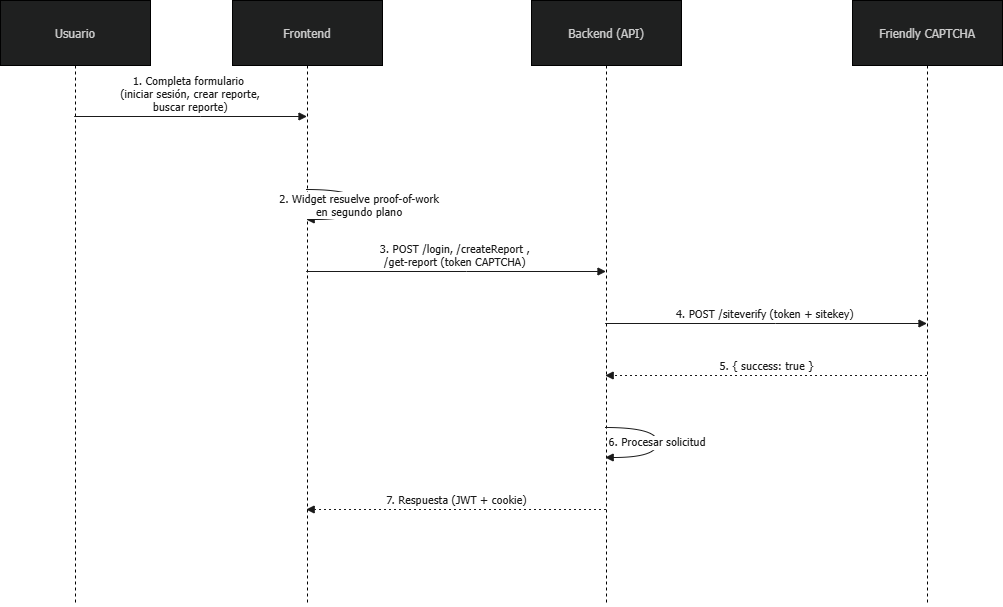
\includegraphics[width=0.85\textwidth]{Graphics/Cap4/captcha_completo.png}
    \caption{Flujo de verificación de Friendly CAPTCHA en endpoints públicos.}
    \label{fig:captcha_flow}
\end{figure}


\subsubsection{Limitación de velocidad}

La limitación de velocidad (en inglés, \textit{rate limiting}) restringe el número de solicitudes que un cliente puede realizar a la API en un período de tiempo determinado. Su propósito es proteger el sistema contra ataques de fuerza bruta, enumeración de recursos y denegación de servicio \cite{microsoft_rate_limiting}. Además, evita que picos de tráfico legítimo o bucles accidentales en el frontend consuman todos los recursos del servidor y degraden la experiencia del resto de usuarios.

Los endpoints públicos del sistema ya cuentan con CAPTCHA como primera barrera, según se describió anteriormente.
El rate limiting actúa como segunda barrera: si un atacante resuelve el CAPTCHA para cada intento, el límite de solicitudes por minuto hace inviable cualquier ataque masivo. Para los endpoints protegidos con JWT, el rate limiting constituye la defensa principal contra el abuso por parte de usuarios autenticados o tokens comprometidos.

\paragraph{Limitación por IP y por sesión}

El sistema aplica un limitador global que contabiliza todas las solicitudes de un mismo cliente, independientemente del endpoint al que se dirijan. Para clientes anónimos —como un reportante que envía un formulario público—, el límite se aplica por dirección IP: 100 solicitudes por minuto. Para usuarios autenticados, el límite se aplica por identificador de sesión extraído del JWT: 200 solicitudes por minuto. Esta diferenciación evita que usuarios legítimos que comparten red —como el personal de un mismo centro de salud— resulten bloqueados por el comportamiento de un tercero, y otorga mayor margen a quienes ya superaron la barrera de autenticación. Una solicitud solo se procesa si el limitador global lo permite.

\paragraph{Políticas complementarias por tipo de operación}

Sobre esta base, el sistema añade políticas específicas que restringen aún más ciertos endpoints según la criticidad de la operación. 
Cada política define un límite de solicitudes, una ventana de tiempo y un comportamiento de encolamiento. 
La ventana fija restablece el contador al cumplirse el intervalo; la ventana deslizante distribuye el límite en segmentos para suavizar los picos de tráfico legítimo. 
El encolamiento permite retener las solicitudes excedentes durante un breve período antes de rechazarlas, lo que evita que un pico puntual de actividad legítima genere errores inmediatos al cliente \cite{microsoft_rate_limiting}.

\begin{itemize}
    \item \texttt{Auth}: 3 solicitudes por minuto para endpoints de autenticación, sin encolamiento. Un usuario legítimo inicia sesión pocas veces al día; tres intentos por minuto bastan para la operación normal y hacen inviable un ataque de fuerza bruta incluso si el atacante resuelve el CAPTCHA en cada intento.
    \item \texttt{Command}: 5 solicitudes por minuto para operaciones de escritura estándar, como la creación de reportes ESAVI, con cola de hasta 5 solicitudes. Equivale a un reporte cada 12 segundos, ritmo suficiente para un centro de salud con múltiples reportantes simultáneos.
    \item \texttt{ReportDaily}: 30 solicitudes por día para la creación de reportes desde una misma IP, mediante ventana deslizante de 24 horas dividida en 24 segmentos. Cubre la actividad diaria de un centro de salud activo y acota el daño máximo de un ataque automatizado a 30 reportes falsos, los cuales pueden identificarse y eliminarse manualmente.
    \item \texttt{CommandDaily}: 20 solicitudes por día para operaciones administrativas como la asignación de reportes o la finalización de revisiones médicas. Refleja el ritmo real de trabajo de un jefe de vacunación municipal o médico evaluador.
    \item \texttt{Query}: 60 solicitudes por minuto para operaciones de lectura, con ventana deslizante dividida en 3 segmentos y cola de hasta 10 solicitudes. Las consultas no modifican el estado del sistema; una consulta por segundo permite una navegación fluida mientras dificulta la extracción masiva de datos.
\end{itemize}

El siguiente fragmento muestra la configuración de dos de estas políticas dentro de la clase \texttt{RateLimitingMiddleware}:

\begin{lstlisting}[language={[Sharp]C}, caption={Configuración de políticas de rate limiting}, label={lst:ratelimiting}]
// Autenticación: muy restrictivo
options.AddFixedWindowLimiter("Auth", config =>
{
    config.PermitLimit = 3;
    config.Window = TimeSpan.FromMinutes(1);
    config.QueueProcessingOrder = QueueProcessingOrder.OldestFirst;
    config.QueueLimit = 0;
});

// Comandos estándar: restrictivo
options.AddFixedWindowLimiter("Command", config =>
{
    config.PermitLimit = 5;
    config.Window = TimeSpan.FromMinutes(1);
    config.QueueProcessingOrder = QueueProcessingOrder.OldestFirst;
    config.QueueLimit = 5;
});
\end{lstlisting}




\paragraph{Aplicación a endpoints}
El atributo \texttt{[EnableRate\-Limiting]} aplica las políticas sobre controladores completos o endpoints específicos. Un mismo endpoint puede combinar múltiples políticas cuando requiere protección en distintas ventanas de tiempo. Por ejemplo, el controlador de autenticación declara únicamente \texttt{Auth} a nivel de clase:

\begin{lstlisting}[language={[Sharp]C}, caption={Aplicación del rate limiting a controladores y endpoints}, label={lst:ratelimitingapplication}]
[ApiController]
[Route("api/[controller]")]
[EnableRateLimiting("Auth")]
public class AuthenticationController : ControllerBase { }
\end{lstlisting}

El endpoint de creación de reportes, en cambio, combina dos políticas: \texttt{Command} limita la tasa por minuto y \texttt{ReportDaily} impone un límite diario por IP. Ambas se evalúan en conjunto con el limitador global: la solicitud solo se procesa si las tres capas lo permiten.

\begin{lstlisting}[language={[Sharp]C}, caption={Combinación de políticas en un mismo endpoint}, label={lst:ratelimitingcombination}]
[HttpPost]
[EnableRateLimiting("Command")]
[EnableRateLimiting("ReportDaily")]
public async Task<IActionResult> Create(CreateReportDto dto) { }
\end{lstlisting}


\paragraph{Alcance de las defensas implementadas}

Aun con estas barreras, un atacante necesitaría resolver múltiples desafíos de proof-of-work y mantenerse por debajo de los umbrales de rate limiting simultáneamente. 
El costo computacional de esta estrategia la vuelve inviable para ataques masivos con los recursos actuales.



















\section{Implementación de la interfaz de usuario}
\label{section:frontend}

El frontend del sistema se construye como una Single Page Application (SPA) en React con TypeScript. La aplicación consume la API REST del backend y ofrece una interfaz accesible tanto para la población que reporta eventos adversos como para el personal del Instituto Finlay que gestiona las revisiones.

\subsection{Arquitectura y enrutamiento}

La aplicación utiliza enrutamiento interno sin depender de librerías externas como React Router. Un componente principal mantiene el estado de la página actual y sincroniza la ruta del navegador con el componente correspondiente mediante un mapa de rutas. Esta decisión reduce el tamaño del bundle final y permite animaciones de transición entre páginas. El acceso a las páginas restringidas se protege mediante un contexto de autenticación que redirige al usuario a la página de inicio de sesión si no hay una sesión activa. Los contextos globales de autenticación y reportes envuelven toda la aplicación y comparten el estado sin necesidad de pasarlo manualmente entre componentes.

\subsection{Gestión del estado y comunicación con la API}

El estado global de autenticación reside en un contexto de React que expone los datos del usuario, el estado de la sesión y las funciones de inicio y cierre de sesión. Al cargar la aplicación, este contexto intenta restaurar la sesión mediante el endpoint de refresco de token, lo que evita que el usuario deba iniciar sesión nuevamente si su token de acceso expiró.

La comunicación con el backend se centraliza en una instancia de Axios configurada con interceptores para la gestión automática de tokens. El interceptor de solicitud inyecta el encabezado de autorización con el token de acceso; el interceptor de respuesta detecta los códigos 401, intenta renovar el token y reenvía la solicitud original. El refresco excluye los endpoints de autenticación para evitar bucles y preserva los encabezados originales en el reintento. Si la renovación falla, la sesión se cierra automáticamente y el usuario regresa a la página de inicio de sesión.

\subsection{Almacenamiento del JWT en memoria}

El token de acceso se mantiene exclusivamente en memoria, sin persistencia en almacenamiento local o de sesión. Esta decisión reduce el riesgo de robo por lecturas desde almacenamiento persistente, aunque no protege contra scripts inyectados que se ejecuten en la página. Por ello, el patrón de seguridad completo combina el token de acceso en memoria con un refresh token almacenado en una cookie HttpOnly, Secure y con SameSite estricta, que el frontend no manipula y por tanto no es vulnerable a ataques de cross-site scripting.

Esta estrategia conlleva un riesgo: el token de acceso se pierde al recargar la página. Para mitigarlo, el contexto de autenticación invoca el endpoint de refresco al cargar la aplicación. Si el refresco tiene éxito, el nuevo token se almacena en memoria y la sesión se restaura sin interrupción para el usuario.

\subsection{Validación en tiempo real}

Los formularios del sistema aplican validación en tiempo real mediante las librerías \texttt{react-hook-form} y \texttt{zod}. La primera reduce el número de renderizaciones al no almacenar el estado de cada campo individualmente, lo que mejora el rendimiento en formularios extensos como el de registro de reportes. La segunda define esquemas declarativos que especifican el formato esperado de cada campo —correo electrónico válido, longitud mínima de contraseña, coincidencia entre campos— y los mensajes de error correspondientes. La integración de ambas permite que el usuario reciba retroalimentación inmediata mientras escribe, sin esperar a enviar el formulario, lo que reduce la cantidad de solicitudes fallidas al backend y mejora la experiencia de uso.

\subsection{Construcción de interfaces de usuario y diseño responsivo}

La interfaz se compone de componentes reutilizables construidos con Tailwind CSS y Radix UI. Tailwind CSS proporciona utilidades de diseño que permiten crear interfaces responsivas sin escribir hojas de estilo personalizadas: las cuadrículas reorganizan sus columnas según el ancho de la pantalla, la navegación alterna entre un menú de escritorio y un menú lateral en dispositivos móviles, y los formularios mantienen un aspecto adecuado en cualquier tamaño de pantalla. Radix UI aporta componentes accesibles —diálogos, selectores, pestañas— que garantizan la compatibilidad con lectores de pantalla y navegación por teclado, en cumplimiento de los requisitos de accesibilidad.

Los gráficos del panel de control utilizan \texttt{recharts}, una librería de visualización de datos para React. Cada gráfico se envuelve en un contenedor responsivo que adapta su tamaño al ancho disponible, y los datos se preprocesan en el backend para reducir el volumen de información transferida al cliente. Los componentes visuales emplean memoización para evitar renderizaciones innecesarias y mantener un rendimiento fluido durante la navegación.

\subsection{Manejo de autenticación en el cliente}

Al iniciar sesión, el cliente decodifica el JWT para extraer el rol del usuario y mostrar únicamente las rutas y opciones correspondientes a ese perfil. 
Esta diferenciación garantiza que cada perfil acceda exclusivamente a las funcionalidades que le corresponden, en cumplimiento de los requisitos de autorización definidos en el Capítulo \ref{chapter:proposal}.



% \section{Implementación del frontend}
% \label{section:frontend}

% El frontend del sistema se construye como una Single Page Application (SPA) en React con TypeScript. La aplicación consume la API REST del backend y ofrece una interfaz accesible tanto para la población que reporta eventos adversos como para el personal del Instituto Finlay que gestiona las revisiones.

% \subsection{Arquitectura y enrutamiento}

% La aplicación utiliza enrutamiento interno controlado por el componente principal \texttt{App.tsx}, que mantiene el estado de la página actual y sincroniza la ruta del navegador con el componente correspondiente mediante un mapa de rutas. Esta decisión evita la dependencia de librerías externas de enrutamiento, reduce el tamaño del bundle final y permite animaciones de transición entre páginas. El acceso a las páginas restringidas se protege mediante el contexto de autenticación (\texttt{AuthContext.tsx}), que redirige al usuario a la página de inicio de sesión si no hay una sesión activa. Los contextos \texttt{AuthProvider} y \texttt{ReportProvider} envuelven toda la aplicación y comparten el estado global sin necesidad de pasarlo manualmente entre componentes.

% \subsection{Gestión del estado y comunicación con la API}

% El estado global de autenticación reside en \texttt{AuthContext.tsx}, que expone los datos del usuario, el estado de la sesión y las funciones de inicio y cierre de sesión. Al cargar la aplicación, el contexto intenta restaurar la sesión mediante el endpoint de refresco de token, lo que evita que el usuario deba iniciar sesión nuevamente si su token de acceso expiró.

% La comunicación con el backend se centraliza en una instancia de Axios (\texttt{api.ts}) configurada con interceptores para la gestión automática de tokens. El interceptor de solicitud inyecta el encabezado \texttt{Authorization} con el token de acceso; el interceptor de respuesta detecta los códigos 401, intenta renovar el token mediante el servicio de autenticación (\texttt{auth.service.ts}) y reenvía la solicitud original. El refresco excluye explícitamente los endpoints de autenticación para evitar bucles, y preserva los encabezados originales en el reintento:

% \begin{lstlisting}[language={TypeScript}, caption={Interceptores de Axios para manejo de tokens (api.ts)}, label={lst:axios}]
% api.interceptors.request.use((config) => {
%     const token = tokenManager.getAccessToken();
%     if (token) config.headers.Authorization = `Bearer ${token}`;
%     return config;
% });

% api.interceptors.response.use(
%     (response) => response,
%     async (error) => {
%         const originalRequest = error.config;
%         if (error.response?.status === 401 
%             && !originalRequest._retry
%             && !originalRequest.url?.includes('/Authentication/')) {
%             originalRequest._retry = true;
%             try {
%                 const { accessToken } = await authService.refreshToken();
%                 tokenManager.setAccessToken(accessToken);
%                 originalRequest.headers.Authorization = `Bearer ${accessToken}`;
%                 return api(originalRequest);
%             } catch (refreshError) {
%                 tokenManager.clearAccessToken();
%                 window.location.href = '/login';
%                 return Promise.reject(refreshError);
%             }
%         }
%         return Promise.reject(error);
%     }
% );
% \end{lstlisting}

% \subsection{Almacenamiento del JWT en memoria}

% El token de acceso se mantiene en memoria mediante el módulo \texttt{token-manager.ts} para evitar su persistencia en \texttt{localStorage} o \texttt{sessionStorage}. Esta decisión reduce el riesgo de robo por lecturas desde almacenamiento persistente, aunque no protege contra scripts inyectados que se ejecuten en la página. Por ello, el patrón de seguridad completo combina el token de acceso en memoria con un refresh token almacenado en una cookie HttpOnly, Secure y con SameSite estricta, que el frontend no manipula y por tanto no es vulnerable a XSS.

% Esta estrategia conlleva un riesgo: el token de acceso se pierde al recargar la página. Para mitigarlo, el contexto de autenticación invoca el endpoint de refresco al cargar la aplicación. Si el refresco tiene éxito, el nuevo token de acceso se almacena en memoria y la sesión se restaura sin que el usuario perciba interrupción alguna. El backend debe reforzar esta protección aplicando tasas límite al endpoint de refresco, rotando los refresh tokens y revocándolos ante uso indebido.

% \subsection{Validación en tiempo real}

% Los formularios del sistema —presentes en páginas como \texttt{login-page.tsx} y \texttt{activate-account-page.tsx}— aplican validación en tiempo real mediante las librerías \texttt{react-hook-form} y \texttt{zod}. \texttt{react-hook-form} reduce el número de renderizaciones al no almacenar el estado de cada campo individualmente, lo que mejora el rendimiento en formularios extensos como el de registro de reportes. \texttt{zod} define esquemas declarativos que especifican el formato esperado de cada campo y los mensajes de error correspondientes. La integración de ambas librerías mediante \texttt{@hookform/resolvers} permite que el usuario reciba retroalimentación inmediata mientras escribe, sin esperar a enviar el formulario:

% \begin{lstlisting}[language={TypeScript}, caption={Validación en tiempo real con react-hook-form y zod}, label={lst:validation}]
% import { useForm } from 'react-hook-form';
% import { z } from 'zod';
% import { zodResolver } from '@hookform/resolvers/zod';

% const schema = z.object({
%     email: z.string().email('Email inválido'),
%     password: z.string().min(8, 'Mínimo 8 caracteres'),
%     confirmPassword: z.string(),
% }).superRefine(({ password, confirmPassword }, ctx) => {
%     if (password !== confirmPassword)
%         ctx.addIssue({
%             code: 'custom',
%             message: 'Las contraseñas no coinciden',
%             path: ['confirmPassword']
%         });
% });

% function AccountForm() {
%     const { register, handleSubmit, formState } = useForm({
%         resolver: zodResolver(schema),
%         mode: 'onChange',
%     });

%     return (
%         <form onSubmit={handleSubmit(onSubmit)}>
%             <input {...register('email')} />
%             {formState.errors.email && <span>{formState.errors.email.message}</span>}
%             <button type="submit" disabled={!formState.isValid}>Enviar</button>
%         </form>
%     );
% }
% \end{lstlisting}

% \subsection{Construcción de interfaces de usuario y diseño responsivo}

% La interfaz se compone de componentes reutilizables construidos con Tailwind CSS y Radix UI, una librería de componentes accesibles que garantiza la compatibilidad con lectores de pantalla y navegación por teclado. Cada página —inicio de sesión, activación de cuenta, panel de reportes, formulario de registro— se implementa como un componente independiente que consume los contextos globales y los servicios de API.

% La responsividad se logra mediante las utilidades de Tailwind CSS. Las cuadrículas reorganizan sus columnas según el ancho de la pantalla, la navegación alterna entre un menú de escritorio y un menú lateral en dispositivos móviles, y los gráficos del panel de control utilizan \texttt{ResponsiveContainer} de \texttt{recharts} para adaptarse automáticamente al tamaño del contenedor. Para garantizar un rendimiento fluido, los datos de los gráficos se preprocesan en el backend y los componentes visuales emplean \texttt{useMemo} para evitar renderizaciones innecesarias. El siguiente fragmento muestra un gráfico de líneas responsivo:

% \begin{lstlisting}[language={TypeScript}, caption={Gráfico responsivo con recharts}, label={lst:recharts}]
% <ResponsiveContainer width="100%" height={300}>
%     <LineChart data={eventsByMonth}>
%         <CartesianGrid strokeDasharray="3 3" />
%         <XAxis dataKey="month" />
%         <YAxis />
%         <Tooltip />
%         <Line type="monotone" dataKey="total" stroke="#0A4B8F" />
%     </LineChart>
% </ResponsiveContainer>
% \end{lstlisting}

% \subsection{Manejo de autenticación en el cliente}

% Al iniciar sesión, el cliente decodifica el JWT para extraer el rol del usuario y mostrar únicamente las rutas y opciones correspondientes a ese rol. El componente de navegación (\texttt{navigation.tsx}) utiliza \texttt{useAuth()} para renderizar menús diferentes según el perfil: un jefe de vacunación ve opciones de asignación y estadísticas; un revisor médico ve únicamente los reportes asignados; un ciudadano solo accede al formulario de reporte público y a la consulta por número de notificación.






% \section{Implementación de funcionalidades principales}
% \label{section:functionalities}

% \subsection{Registro de reportes de ESAVI}

% \subsection{Gestión de revisiones médicas}

% \subsection{Asignación de responsables}

% \subsection{Gestión de causalidad}

% \subsection{Sistema de notificaciones}

% \subsection{Visualización y consulta de reportes}

\section{Despliegue de la solución}
\label{section:deployment}

El sistema se despliega en dos entornos diferenciados. Para desarrollo local, un archivo \texttt{docker-compose.yml} levanta los servicios de RabbitMQ y la API, mientras que la base de datos MySQL se ejecuta en el servidor local. 
Para demostración y pruebas, la API se despliega en Railway, una plataforma como servicio que automatiza la construcción y publicación desde el repositorio de GitHub. 

La configuración se centraliza en un \texttt{Dockerfile} multietapa\footnote{Multietapa: técnica que divide la construcción en fases con imágenes base distintas, reduciendo el tamaño final.} que compila la aplicación en una imagen de SDK\footnote{SDK: imagen con compilador y herramientas de desarrollo.} y la publica en una imagen de runtime\footnote{Runtime: imagen solo con las bibliotecas para ejecutar la aplicación.}, y en variables de entorno que inyectan las credenciales de base de datos, las claves de JWT y las API keys de los servicios externos sin exponerlas en el código fuente.

La migración a servidores físicos del Instituto Finlay, prevista para la etapa de producción, mantendrá la misma configuración de contenedores y variables de entorno, lo que garantiza que el entorno de producción sea idéntico al de desarrollo.



\section{Conclusiones del capítulo}
\label{section:chapter_conclusions}

En este capítulo se presentaron los principales detalles relacionados con la implementación de la plataforma desarrollada, describiendo las tecnologías empleadas, la organización arquitectónica de la solución y los mecanismos utilizados en el backend y el frontend. Además, se abordaron aspectos asociados a la seguridad, la integración entre componentes y el despliegue del sistema, evidenciando la materialización práctica de la propuesta presentada en el capítulo anterior.

\chapter{Validación de la aplicación}\label{chapter:result}


% \section{Propósito de la validación}

% La validación del sistema persigue demostrar cuatro afirmaciones concretas:

% \begin{enumerate}
%     \item \textbf{Los flujos principales operan correctamente.} El registro de reportes, la asignación a revisores, la gestión de revisiones y las notificaciones automáticas funcionan conforme a los requerimientos funcionales definidos en el Capítulo \ref{chapter:proposal}.
%     \item \textbf{El sistema responde en menos de 5 segundos.} El envío de un reporte completo —desde la recepción de la solicitud hasta la respuesta de confirmación— no supera el límite establecido en el RNF-05, excluyendo la latencia de red externa.
%     \item \textbf{Los mecanismos de seguridad operan según lo diseñado.} Los endpoints protegidos rechazan solicitudes sin token, con token expirado o con rol insuficiente; el rate limiting bloquea el exceso de solicitudes; y el CAPTCHA impide el envío automatizado de formularios.
%     \item \textbf{Los usuarios finales consideran la interfaz útil y fácil de usar.} La evaluación mediante el cuestionario SUS (System Usability Scale) debe arrojar una puntuación superior a 68, umbral que define la usabilidad aceptable según el estándar del cuestionario \cite{brooke1996sus}.
% \end{enumerate}

% \section{Entorno y metodología}

% \subsection{Hardware}

% Las pruebas se ejecutaron sobre una máquina con las siguientes características:

% \begin{itemize}
%     \item \textbf{Procesador:} Intel Core i5-8250 CPU @ 1.80GHz
%     \item \textbf{Memoria RAM:} 16 GB DDR4
%     \item \textbf{Almacenamiento:} SSD KINGSTON de 512 GB
% \end{itemize}

% \subsection{Software}

% El entorno de pruebas replicó la configuración de desarrollo local definida en el Capítulo \ref{chapter:implementation}:

% \begin{itemize}
%     \item \textbf{Sistema operativo:} Windows 11 Pro

%     \item \textbf{Base de datos:} MySQL 8.0
%     \item \textbf{Backend:} .NET 8, ejecutado mediante Docker Compose
%     \item \textbf{Frontend:} Vite + React 18, ejecutado en modo desarrollo
%     \item \textbf{Navegador:} Google Chrome 124
% \end{itemize}

% \subsection{Red}

% Todas las pruebas se ejecutaron en entorno local, con la API y la base de datos corriendo en la misma máquina. Esta configuración excluye la latencia de red externa de las mediciones de rendimiento, conforme al RNF-05.

% \subsection{Datos de prueba}

% La base de datos se pobló con datos sintéticos que simulan el escenario real del Instituto Finlay:

% \begin{itemize}
%     \item \textbf{Provincias y municipios:} 16 provincias y 32 municipios, correspondientes a la división político-administrativa de Cuba.
%     \item \textbf{Vacunas:} 5 vacunas activas con sus respectivos fabricantes.
%     \item \textbf{Síntomas:} 15 síntomas activos.
%     \item \textbf{Usuarios:} 1 administrador, 2 jefes de vacunación municipales, 3 médicos evaluadores y 2 ciudadanos de prueba.
%     \item \textbf{Reportes:} 20 reportes de ESAVI con distintos estados, severidades y asignaciones.
% \end{itemize}

% \subsection{Metodología}

% La validación combinó cuatro enfoques complementarios:

% \begin{itemize}
%     \item \textbf{Pruebas funcionales manuales:} ejecución de los flujos principales del sistema por parte del desarrollador, verificando que cada paso produce el resultado esperado según los requerimientos funcionales.
%     \item \textbf{Pruebas unitarias automatizadas:} validación de reglas de negocio mediante xUnit sobre los validadores de la capa de aplicación, con dependencias simuladas.
%     \item \textbf{Pruebas de rendimiento:} medición de tiempos de respuesta con K6, ejecutando 100 solicitudes por endpoint.
%     \item \textbf{Pruebas de usabilidad:} evaluación con usuarios representativos mediante el método de pensamiento en voz alta y el cuestionario SUS.
% \end{itemize}

\section{Pruebas funcionales}

Las pruebas funcionales verificaron que los flujos principales del sistema operan conforme a los requerimientos funcionales definidos en el Capítulo \ref{chapter:proposal}. La Tabla \ref{tab:pruebas_funcionales} resume los casos de prueba ejecutados, seleccionados por su representatividad dentro del flujo de farmacovigilancia.

\begin{table}[H]
\centering
\caption{Resumen de casos de prueba funcionales}
\label{tab:pruebas_funcionales}
\begin{tabular}{|p{1.2cm}|p{3.5cm}|p{3.5cm}|p{3cm}|c|}
\hline
\textbf{ID} & \textbf{Caso de prueba} & \textbf{Datos de entrada} & \textbf{Resultado esperado} & \textbf{¿Pasó?} \\
\hline
CP01 & Registro de reporte público & Datos completos de sujeto, vacuna y síntoma & Código 201 y número de notificación & \checkmark \\
\hline
CP02 & Registro con campos vacíos & Formulario sin datos obligatorios & Código 400 con errores de validación & \checkmark \\
\hline
CP03 & Inicio de sesión con credenciales válidas & Correo y contraseña correctos & JWT, cookie de refresh y redirección al panel & \checkmark \\
\hline
CP04 & Inicio de sesión con credenciales inválidas & Correo y contraseña incorrectos & Código 400 con mensaje de error & \checkmark \\
\hline
CP05 & Asignación de reporte a revisor & Reporte pendiente y revisor disponible & Asignación creada y notificación enviada & \checkmark \\
\hline
CP06 & Consulta de reportes por municipio & Municipio con 5 reportes registrados & Lista con 5 reportes & \checkmark \\
\hline
CP07 & Finalización de revisión médica & Reporte en estado: \textit{En revisión} & Estado actualizado a \texttt{Revisado} & \checkmark \\
\hline
CP08 & Exportación de reporte a PDF & Reporte con datos completos & Archivo PDF generado correctamente & \checkmark \\
\hline
CP09 & Consultar estado de reporte válido & Número de notificación & Estado detallado & \checkmark \\
\hline
\end{tabular}
\end{table}


\section{Pruebas de rendimiento}

\section{Pruebas de usabilidad}

\section{Discusión de resultados}

\section{Resumen de hallazgos}

\backmatter

  \begin{conclusions}
   
% El desarrollo del sistema de autorreporte de eventos adversos a vacunas para el Instituto Finlay de Vacunas permitió materializar los objetivos planteados al inicio de este trabajo. A continuación se sintetizan los principales logros alcanzados:

% \begin{itemize}
%     \item \textbf{Se diseñó e implementó una arquitectura limpia en capas} que separa el dominio, la aplicación, la infraestructura y la presentación. Esta arquitectura permitió migrar entre proveedores de correo electrónico sin modificar la lógica de negocio e incorporar nuevos mecanismos de notificación sin afectar los casos de uso existentes.

%     \item \textbf{Se desarrolló una API REST segura} con autenticación basada en JWT con refresh tokens en cookies HttpOnly, autorización por roles, protección contra ataques automatizados mediante CAPTCHA y rate limiting, y validación de solicitudes en dos niveles —formato y reglas de negocio—.

%     \item \textbf{Se construyó un sistema de notificaciones asíncrono} que desacopla el envío de correos de la lógica de negocio mediante RabbitMQ, lo que permitió que el usuario reciba respuesta inmediata mientras las notificaciones se procesan en segundo plano.

%     \item \textbf{Se implementó una interfaz de usuario responsiva} que permite a la población reportar eventos adversos sin autenticación previa, y al personal del IFV gestionar revisiones y asignaciones según su perfil, con validación en tiempo real y almacenamiento seguro del token de acceso.

%     \item \textbf{Se contenerizó la solución con Docker} y se desplegó en Railway y Vercel para facilitar las pruebas remotas por parte de los investigadores del IFV, con la misma configuración prevista para la migración a servidores físicos institucionales.
% \end{itemize}

% La experiencia adquirida a lo largo de este proyecto abarcó desde el análisis de requisitos con expertos del dominio hasta la implementación de mecanismos de seguridad con fundamento criptográfico, pasando por la selección de tecnologías adecuadas al contexto cubano. El sistema resultante constituye una base funcional sobre la cual el Instituto Finlay puede construir las próximas iteraciones que se describen a continuación.


El desarrollo del sistema permitió materializar los objetivos planteados al inicio de este trabajo. Los principales logros alcanzados fueron:

\begin{itemize}
    \item \textbf{Una arquitectura limpia en capas} que separa el dominio, la aplicación, la infraestructura y la presentación, y permitió migrar entre proveedores de correo sin modificar la lógica de negocio.

    \item \textbf{Una API REST segura} con autenticación basada en JWT, autorización por roles, CAPTCHA, rate limiting y validación en dos niveles.

    \item \textbf{Un sistema de notificaciones asíncrono} que desacopla el envío de correos mediante RabbitMQ, permitiendo que el usuario reciba respuesta inmediata.

    \item \textbf{Una interfaz de usuario responsiva} para que la población reporte eventos adversos y el personal del IFV gestione revisiones y asignaciones según su perfil.

    \item \textbf{La contenerización de la solución con Docker} y su despliegue en Railway y Vercel, con la misma configuración prevista para servidores físicos institucionales.
\end{itemize}

La experiencia abarcó desde el análisis de requisitos con expertos del dominio hasta la implementación de mecanismos de seguridad con fundamento criptográfico, pasando por la selección de tecnologías adecuadas al contexto cubano. El sistema resultante constituye una base funcional sobre la cual el Instituto Finlay puede construir las próximas iteraciones.


\end{conclusions}

  \begin{recomendations}
\label{ref:recomendations}

Frente a las limitaciones identificadas, las siguientes acciones permitirán llevar el sistema a su pleno potencial operativo:

\begin{enumerate}
    \item \textbf{Migrar los canales de notificación a producción.} Reemplazar EmailJS y OpenWA por un servidor SMTP institucional y la API oficial de WhatsApp Business, incorporando SMS como canal complementario para usuarios sin datos móviles.

    \item \textbf{Completar las pruebas de usabilidad con médicos y jefes municipales.} Aplicar el recorrido cognitivo y el cuestionario SUS a al menos 3 participantes de cada perfil en sesiones presenciales, registrando tiempos de ejecución y tasa de errores.

    \item \textbf{Replicar las pruebas de rendimiento en infraestructura institucional.} Ejecutar nuevamente las pruebas de carga sobre los servidores físicos del IFV para obtener umbrales reales, sin las limitaciones del entorno de desarrollo.

    \item \textbf{Optimizar los recursos estáticos del frontend.} Aplicar las mejoras detectadas por Lighthouse: compresión de imágenes a formatos WebP, eliminación de JavaScript no utilizado y precarga de estilos críticos.

    \item \textbf{Implementar fusión inteligente de duplicados.} Al confirmar un duplicado, preservar los datos únicos de la copia en el reporte original, siempre bajo supervisión del jefe de vacunación.

    \item \textbf{Migrar a servidores físicos del Instituto Finlay.} Trasladar el sistema desde Railway y Vercel a los servidores institucionales utilizando la misma configuración de contenedores Docker, garantizando el control sobre los datos de farmacovigilancia.

    \item \textbf{Desarrollar una aplicación móvil nativa.} Evaluar la creación de una aplicación para iOS y Android que aproveche notificaciones push y acceso sin conexión, apoyándose en la API actual sin requerir modificaciones.
\end{enumerate}

\end{recomendations}
\appendix

% \chapter{Resultados de farmacovigilancia pasiva en Cuba y las Américas}

% \section{Reporte de RAM notificadas por farmacovigilancia pasiva en Cuba}
% \label{app:reportes_cuba_2020}

% En el Anexo~\ref{app:reportes_cuba_2020} se presenta una figura con la evolución de las notificaciones de reacciones adversas a medicamentos (RAM) en Cuba entre 2014 y 2020. Estos datos corresponden al sistema de \textbf{farmacovigilancia pasiva}, basado en la notificación espontánea de sospechas de RAM por parte del personal sanitario.

% \begin{figure}[H]
%     \centering
%     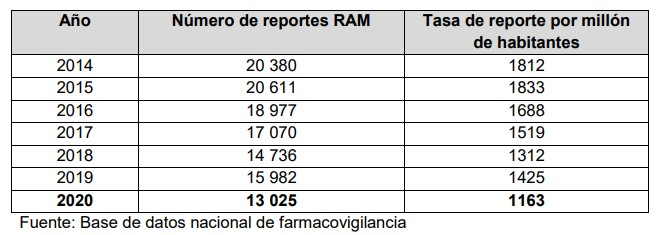
\includegraphics[scale=1.2]{Graphics/Cap1/ram_en_cuba_2020.jpg}
%     \caption{Notificaciones de \gls{reacción adversa a medicamentos (RAM)} declaradas mediante farmacovigilancia pasiva en Cuba (2014-2020). Fuente: \gls{cecmed}, Informe Anual 2020 \cite{cecmed_farmacovigilancia_cuba_2020}.}
%     \label{fig:reporte_ram_cuba_2020}
% \end{figure}

% \section{Reporte según grupo farmacológico}
% \label{app:grupo_farmacologico}

% En el Anexo~\ref{app:grupo_farmacologico} se incluye una figura que muestra los reportes de \gls{reacción adversa a medicamentos (RAM)} según el grupo farmacológico, a partir de la farmacovigilancia pasiva del año 2020.

% \begin{figure}[H]
%     \centering
%     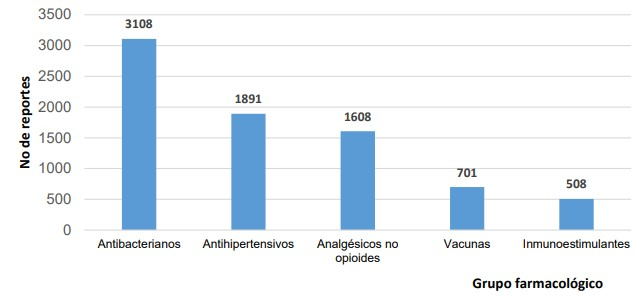
\includegraphics[scale=1.5]{Graphics/Cap1/grupo_farmacologico.jpg}
%     \caption{Reporte de \gls{reacción adversa a medicamentos (RAM)} según grupo farmacológico. Farmacovigilancia pasiva, 2020. Adaptado de \cite{cecmed_farmacovigilancia_cuba_2020}}
%     \label{fig:grupo_farmacologico_ram}
% \end{figure}



% \section{Notificaciones de ESAVI por países de la región de las Américas}
% \label{app:esavi_por_paises}

% En el Anexo~\ref{app:esavi_por_paises} se incluye una figura que presenta el número de \gls{esavi} notificados por los países de la región de las Américas.

% \begin{figure}[H]
%     \centering
%     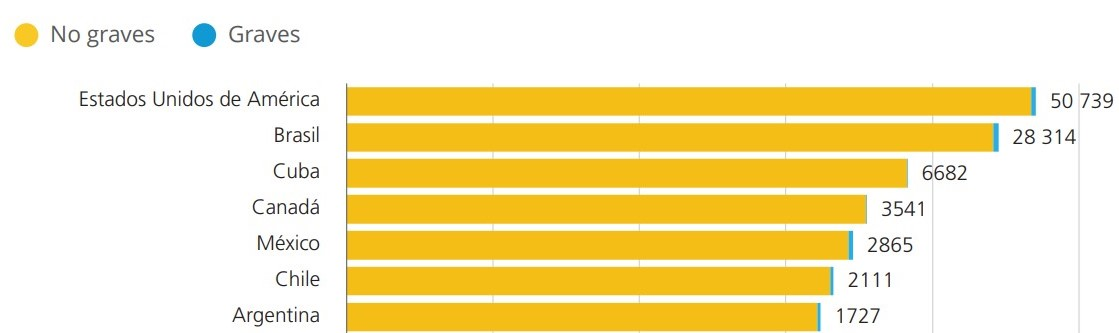
\includegraphics[scale=0.8]{Graphics/Cap1/copia_paises_ram.jpg}
%     \caption{Número de \gls{esavi} notificados por los países de la región de las Américas. Adaptado de \cite{ops_manual_esavi_2021}}
%     \label{fig:esavi_paises_americas}
% \end{figure}

% \section{Estructura del Sistema de Vigilancia de Medicamentos en Cuba}
% \label{app:estructura_vigilancia}

% En el Anexo~\ref{app:estructura_vigilancia} se incluye una figura que presenta la organización del sistema cubano de vigilancia de medicamentos.

% \begin{figure}[htbp]
%     \centering
%     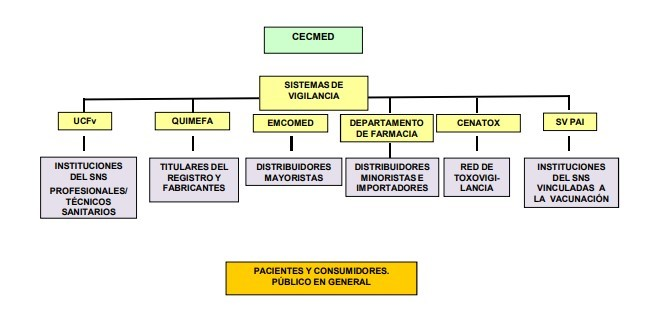
\includegraphics[scale=1.2]{Graphics/Cap1/estructura_vigilancia_medicamentos_cuba2.jpg}
%     \caption{Estructura del Sistema de Vigilancia de Medicamentos en Cuba. Adaptado de: \cite{paho_vigilancia_medicamentos_cuba}}
%     \label{fig:estructura_vigilancia_medicamentos_cuba}
% \end{figure}


% El sistema de vigilancia de medicamentos en Cuba se estructura bajo la rectoría del \gls{cecmed}, autoridad reguladora nacional encargada de la evaluación, control y toma de decisiones sobre la seguridad de los medicamentos a partir de la información generada en el sistema.

% Para el cumplimiento de estas funciones, se articula una red de vigilancia integrada por diversos componentes que interactúan de manera coordinada (ver Figura \ref{fig:estructura_vigilancia_medicamentos_cuba}) \cite{paho_vigilancia_medicamentos_cuba}:

% \begin{itemize} 
%     \item \textbf{\gls{ucnfv} (\gls{minsap}):} Cohesiona la Red de Farmacoepidemiología en los 169 municipios del país y actúa como el canal central para la \gls{notificación espontánea} de profesionales y pacientes, siendo las vacunas la excepción gestionada de forma especializada por el \gls{pai} \cite{paho_vigilancia_medicamentos_cuba,normas_farmacovigilancia_cuba_2012}. 
%     \item \textbf{Fabricantes y Titulares de Registro (QUIMEFA):} Involucra a las 24 empresas farmacéuticas nacionales, donde cada una cuenta con personal designado para la vigilancia y reporta directamente sobre la seguridad y calidad de sus productos \cite{paho_vigilancia_medicamentos_cuba}. 
%     \item \textbf{Distribución Mayorista (EMCOMED):} Coordina la vigilancia en las 24 droguerías del país, detectando problemas de calidad durante el almacenamiento y transportación \cite{paho_vigilancia_medicamentos_cuba}. 
%     \item \textbf{Distribución Minorista (Departamento de Farmacia):} Supervisa la vigilancia en las más de 2,000 farmacias comunitarias y hospitalarias del Sistema Nacional de Salud \cite{paho_vigilancia_medicamentos_cuba}.  
%     \item \textbf{\gls{cenatox}:} Lidera la red de toxicovigilancia, supervisando las intoxicaciones y reacciones adversas de naturaleza \gls{toxica} \cite{paho_vigilancia_medicamentos_cuba}. 
%     \item \textbf{SV \gls{pai}:} Realiza la vigilancia especializada de vacunas mediante el monitoreo de los \gls{esavi}, bajo la supervisión del Viceministerio de Higiene y Epidemiología \cite{paho_vigilancia_medicamentos_cuba}. 
% \end{itemize}

% Toda la información captada por estos efectores fluye hacia el Observatorio de Vigilancia Postcomercialización del \gls{cecmed}, donde se evalúa la relación beneficio-riesgo para emitir alertas farmacológicas, retirar lotes o modificar registros sanitarios en tiempo real \cite{paho_vigilancia_medicamentos_cuba}. 



























% \chapter{Modelos oficiales de notificación en Cuba}
% \label{app:modelos_formularios}

% \section{Modelo 33-36-02}
% \label{app:modelo_33-36-02}

% En el Anexo \ref{app:modelo_33-36-02} se incluye el \textbf{Modelo 33-36-02}, el formulario oficial utilizado por los profesionales de la salud en Cuba para la notificación de sospechas de reacciones adversas a medicamentos dentro del sistema nacional de farmacovigilancia.

% \begin{figure}[H]
%     \centering
%     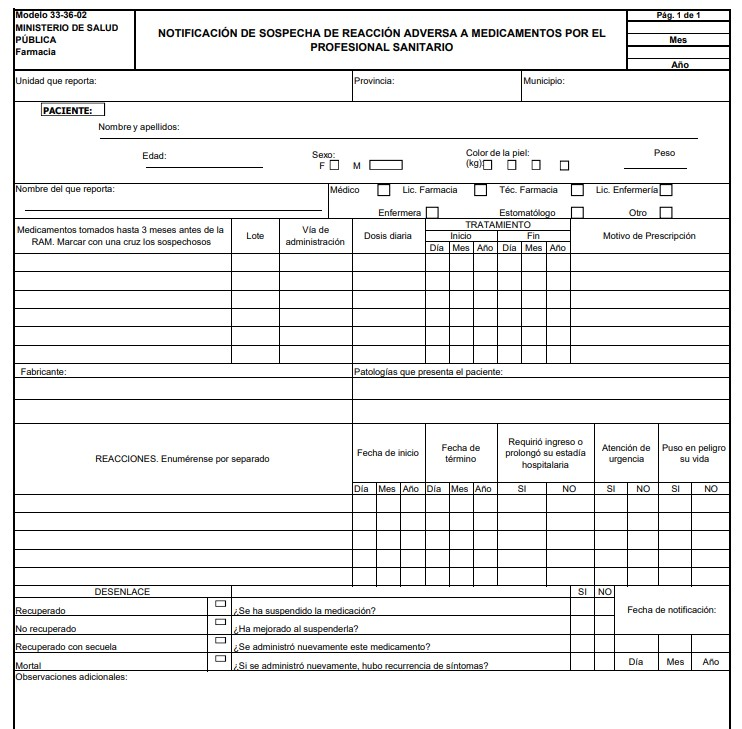
\includegraphics[width=\textwidth]{Graphics/Cap1/modelo_cubano_33_36_02.jpg}
%     \caption{Modelo 33-36-02: Notificación de sospechas de Reacciones Adversas a Medicamentos por el Profesional Sanitario. Adaptado de \cite{normas_farmacovigilancia_cuba_2012}}
% \end{figure}

% % El formulario incluye instrucciones detalladas para la notificación de reacciones adversas, abarcando desde la identificación del medicamento sospechoso hasta la descripción clínica del evento, con el objetivo de garantizar la completitud y calidad de los reportes dentro del sistema de farmacovigilancia.
% \newpage

% \begin{figure}[H]
%     \centering
%     
\includegraphics[width=\textwidth]{Graphics/Cap1/dorso_modelo_33_36_02.jpg}
%     \caption{Instructivo en el dorso del modelo 33-36-02: Notificación de sospechas de Reacciones Adversas a Medicamentos por el Profesional Sanitario, Adaptado de \cite{normas_farmacovigilancia_cuba_2012}}
% \end{figure}

% \newpage

% \section{Modelo 33-36-03}
% \label{app:modelo_33-36-03}

% En el Anexo \ref{app:modelo_33-36-03} se incluye el \textbf{Modelo 33-36-03}, el formulario oficial utilizado por los pacientes en Cuba para la notificación de sospechas de reacciones adversas a medicamentos dentro del sistema nacional de farmacovigilancia.

% \begin{figure}[H]
%     \centering
%     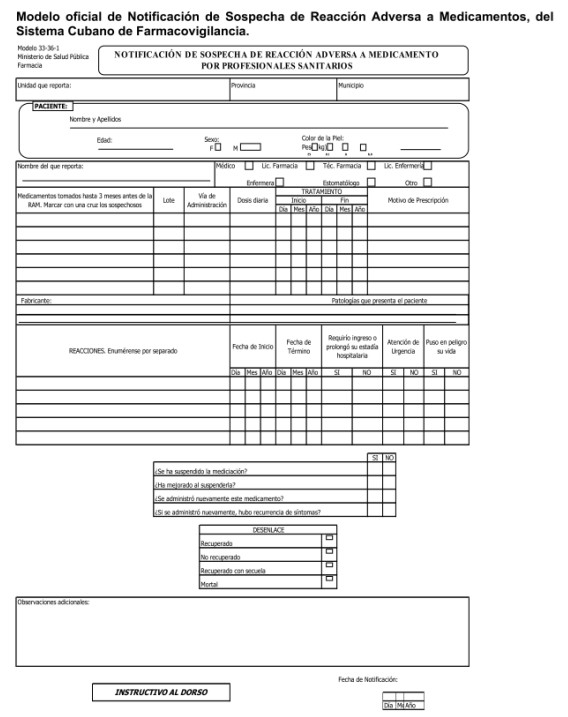
\includegraphics[width=\textwidth]{Graphics/Cap1/modelo_33_36_03.jpg}
%     \caption{Modelo 33-36-03: Notificación de sospechas de Reacciones Adversas a Medicamentos por el Paciente. Adaptado de \cite{normas_farmacovigilancia_cuba_2012}}
% \end{figure}


% \begin{figure}[H]
%     \centering
%     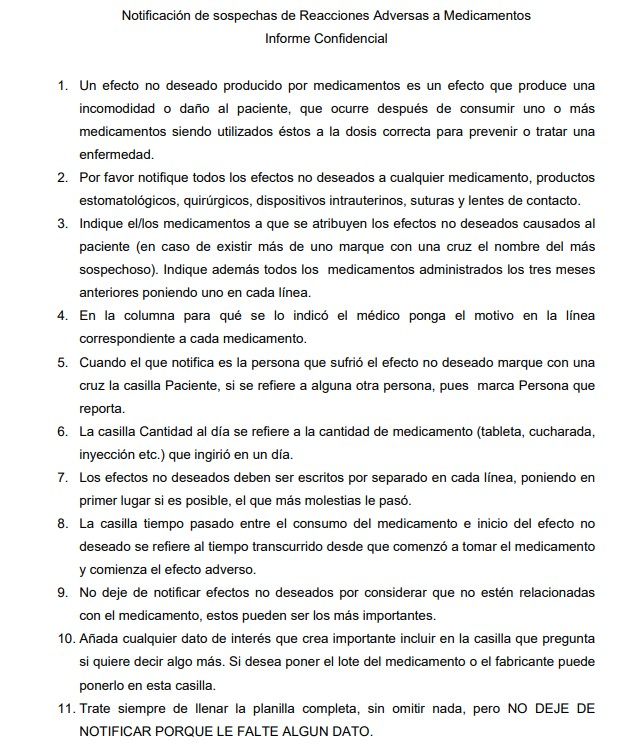
\includegraphics[width=\textwidth]{Graphics/Cap1/dorso_modelo_33_36_03.jpg}
%     \caption{Instructivo en el dorso del modelo 33-36-03: Notificación de sospechas de Reacciones Adversas a Medicamentos por el Paciente. Adaptado de \cite{normas_farmacovigilancia_cuba_2012}}
% \end{figure}


% \newpage

% \section{Modelo 84-30-2}
% \label{app:modelo_84-30-2}
% En el Anexo \ref{app:modelo_84-30-2} se incluye el \textbf{Modelo 84-30-2}, el formulario oficial utilizado por los profesionales de la salud en Cuba para la notificación de sospechas de eventos supuestamente atribuibles a la vacunación o inmunización (ESAVI) dentro del sistema nacional de farmacovigilancia.

% \begin{figure}[H]
%     \centering
%     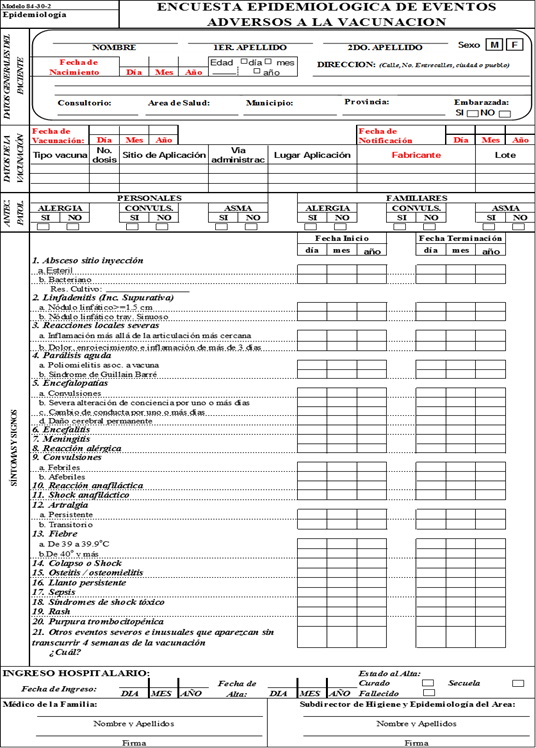
\includegraphics[width=\textwidth]{Graphics/Cap1/modelo_84_30_2.png}
%     \caption{Modelo 84-30-2: Notificación de sospechas de Eventos Supuestamente Atribuibles a la Vacunación o Inmunización (ESAVI). Adaptado de \cite{cecmed_ar_00_515}}
% \end{figure}




% \newpage
% \chapter{Base de Datos Central de Farmacovigilancia (FarmaVigiC)}

% \section{Campos de la base de datos central de farmacovigilancia (FarmaVigiC)}
% \label{app:base_datos_farmavigic}

% En el Anexo \ref{app:base_datos_farmavigic} se describen los campos de la base de datos central de farmacovigilancia (FarmaVigiC) utilizada en Cuba.

% \renewcommand{\arraystretch}{1.3}

% \begin{longtable}{|p{3.2cm}|p{9.3cm}|}
% \caption{Campos de la base de datos central de farmacovigilancia (FarmaVigiC). Elaboración propia a partir de \cite{normas_farmacovigilancia_cuba_2012} (p. 42).}
% \label{tab:base_datos_farmavigic}\\

% \hline
% \textbf{Grupos de campos} & \textbf{Variables o campos} \\
% \hline
% \endfirsthead

% \hline
% \textbf{Grupos de campos} & \textbf{Variables o campos} \\
% \hline
% \endhead
		

% \hline
% \endfoot

		
% 		Paciente & \makecell[l]{Nombre y apellidos\\Edad\\Sexo \\ Raza \\ Antecedentes patológicos personales \\ Requirió ingreso \\ Requirió atención de urgencia \\ Requirió reposo \\ Fue baja laboral o escolar \\ Peligró su vida} \\
%         \hline

%         Notificador & \makecell[l]{Unidad que reporta\\Provincia\\Municipio\\Nombre y apellidos \\ Especialidad} \\
%         \hline

%         Medicamentos & \makecell[l]{Medicamento sospechoso\\Presentación cantidad\\Presentación unidad\\Forma farmacéutica\\Fabricante\\Diluyente\\Lote\\ Vía de administración \\ Dosis cantidad \\ Dosis unidad \\ Dosis frecuencia \\ Fecha de inicio del tratamiento \\ Fecha fin del tratamiento \\ Continuación \\ Motivo de prescripción \\ Otro fármaco 1 \\ Otro fármaco 2 \\ Otro fármaco 3 \\ Otro fármaco 4 \\ Otro fármaco 5 \\ Otro fármaco 6 \\ Vía, dosis, lote de otros fármacos \\ Fecha de administración de otros fármacos} \\
%         \hline

%         Reacciones adversas & \makecell[l]{Reacción principal\\Otra RAM 1\\Otra RAM 2\\Otra RAM 3\\Otra RAM 4\\Otra RAM 5\\Otra RAM 6 \\ Fecha de inicio RAM \\ Fecha fin de RAM \\ Continuación} \\[6pt]
% 		\hline
		
% 		Clasificación & \makecell[l]{Grupo de edades\\Sexo\\Nivel de atención\\Especialidad\\Grupo farmacológico\\Sistema de órgano afectado\\Severidad\\Causalidad\\Importancia\\Frecuencia} \\[6pt]
% 		\hline
		
% 		Desenlace & \makecell[l]{Suspendió la medicación\\Supresión positiva\\Re exposición\\Recurrencia de síntomas\\Desenlace\\Recuperado\\No recuperado \\ Recuperado con secuela} \\[6pt]
% 		\hline

%         Organización e información adicional & \makecell[l]{Mes de entrada a la base\\Secuencia temporal\\Observaciones\\Comentarios\\Resultados de necropsia\\Fecha de notificación} \\[6pt]
% 		\hline

%         Evaluación de la calidad & \makecell[l]{E1 (evalúa al notificador)\\E2 (evalúa al revisor) \\ E3 (evalúa calidad del llenado de la base)} \\[6pt]
% 		\hline
	
% \end{longtable}

% \begin{itemize}
%     \item A nivel municipal se trabajan 71 campos
%     \item A nivel provincial se trabajan 72 campos
%     \item A nivel nacional se trabajan 75 campos
% \end{itemize}

% \newpage

% \chapter{Formularios de referencia}

% \section{Formulario VAERS - Octubre 2025}
% \label{app:vaers-form-oct2025}

% En el Anexo \ref{app:vaers-form-oct2025} se incluye el formulario oficial del Vaccine Adverse Event Reporting System (VAERS) correspondiente a octubre de 2025. Este formulario constituye el instrumento estándar utilizado para la notificación de eventos adversos posteriores a la vacunación en los Estados Unidos.

% \begin{figure}[H]
%     \centering
%     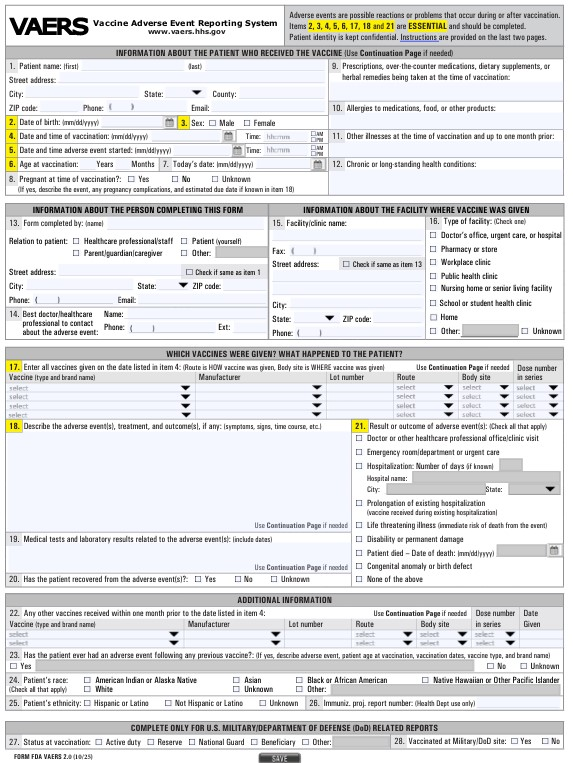
\includegraphics[width=\textwidth]{Graphics/Cap2/vaers-formulario.jpg}
%     \caption{Formulario VAERS - Octubre 2025}
% \end{figure}


% \newpage



% \section{Formulario v-safe - Enero 2021}
% \label{app:vsafe-form-ene2021}

% En el Anexo \ref{app:vsafe-form-ene2021} se incluyen capturas del sistema v-safe del CDC correspondientes a enero de 2021. 
% Este sistema constituye una herramienta de seguimiento activo utilizada para monitorizar síntomas y eventos adversos posteriores a la vacunación.

% \begin{figure}[htpb]
%     \centering
    
%     % Fila 1
%     \begin{minipage}[t]{0.45\textwidth}
%         \centering
%         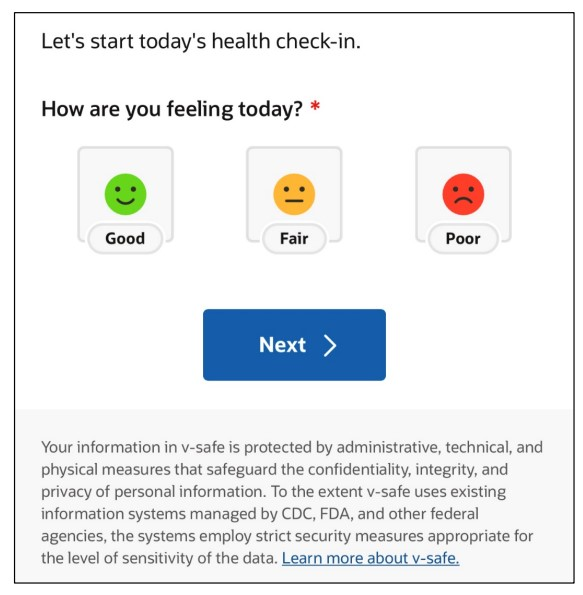
\includegraphics[width=\linewidth]{Graphics/Cap2/feeling.jpg}
%         \caption{Estado general}
%     \end{minipage}
%     \hfill
%     \begin{minipage}[t]{0.45\textwidth}
%         \centering
%         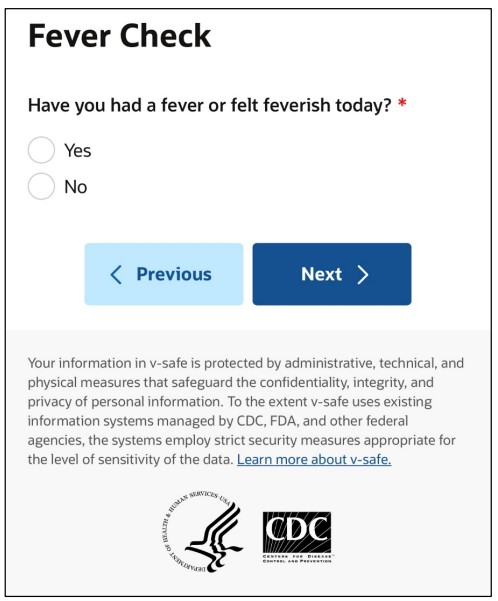
\includegraphics[width=\linewidth]{Graphics/Cap2/fever.jpg}
%         \caption{Verificación de fiebre}
%     \end{minipage}

%     \vspace{0.5cm}
    
%     % Fila 2
%     \begin{minipage}[t]{0.45\textwidth}
%         \centering
%         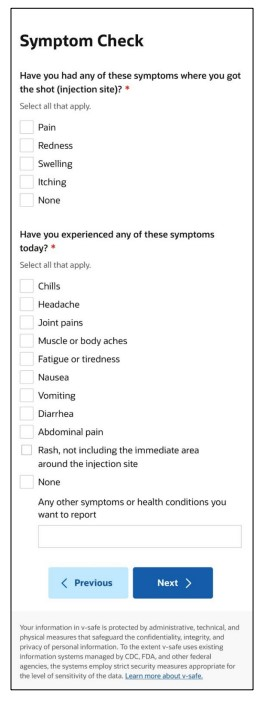
\includegraphics[width=0.5\linewidth]{Graphics/Cap2/symptom.jpg}
%         \caption{Verificación de síntomas}
%     \end{minipage}
%     \hfill
%     \begin{minipage}[t]{0.45\textwidth}
%         \centering
%         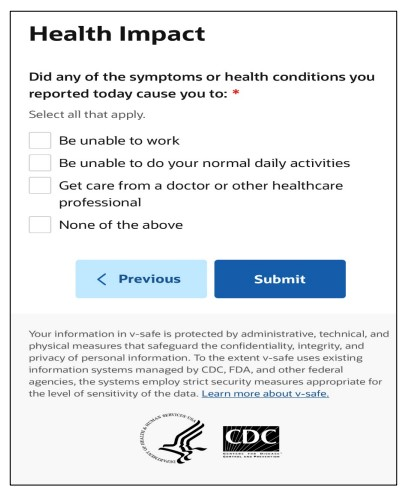
\includegraphics[width=\linewidth]{Graphics/Cap2/health.jpg}
%         \caption{Impacto en la salud}
%     \end{minipage}

%     \caption{Capturas del sistema v-safe para el seguimiento de síntomas posteriores a la vacunación}
%     \label{fig:vsafe-form}
% \end{figure}












% \chapter{Entidades de infraestructura}
% \label{anexo:entidades_infraestructura}

% \section{RefreshToken}

% La entidad \texttt{RefreshToken} permite la renovación de sesiones sin que el usuario deba iniciar sesión nuevamente. Cuando un usuario se autentica, el sistema genera un token de acceso JWT de corta duración y un token de actualización que persiste en esta tabla. Al expirar el token de acceso, el cliente presenta el token de actualización y obtiene uno nuevo.

% \begin{lstlisting}[language={[Sharp]C}, caption={Entidad RefreshToken}, label={lst:refreshtoken}]
% public class RefreshToken : GuidEntity
% {
%     public string Token { get; set; } = null!;
%     public DateTime ExpiresAt { get; set; }
%     public bool Revoked { get; set; }
%     public Guid UserId { get; set; }
%     public User User { get; set; } = null!;
% }
% \end{lstlisting}

% \texttt{Token} almacena el valor del token de actualización. \texttt{ExpiresAt} define su vencimiento. \texttt{Revoked} permite invalidarlo antes de esa fecha. \texttt{UserId} y \texttt{User} asocian cada token con su usuario.


% \section{AuditLog}

% La entidad \texttt{AuditLog} registra las operaciones realizadas sobre el sistema y constituye la base para las funcionalidades de auditoría y trazabilidad descritas en la sección \ref{section:backend} del Capítulo 4. Contempla tanto usuarios autenticados como reporteros anónimos.

% \begin{table}[H]
% \centering
% \caption{Campos de la entidad \texttt{AuditLog}}
% \label{tab:auditlog}
% \begin{tabular}{|l|l|p{6cm}|}
% \hline
% \textbf{Campo} & \textbf{Tipo} & \textbf{Descripción} \\
% \hline
% \texttt{UserId} & \texttt{Guid?} & Usuario autenticado (nulo si es anónimo) \\
% \texttt{UserEmail} & \texttt{string?} & Correo del usuario autenticado \\
% \texttt{ReporterName} & \texttt{string?} & Nombre del reportero anónimo \\
% \texttt{ReporterEmail} & \texttt{string?} & Correo del reportero anónimo \\
% \texttt{Action} & \texttt{string} & Operación: Create, Update, Delete, View \\
% \texttt{EntityName} & \texttt{string} & Entidad afectada (ej. AefiReport) \\
% \texttt{EntityId} & \texttt{Guid?} & Identificador del registro afectado \\
% \texttt{Details} & \texttt{string?} & Descripción legible de la acción \\
% \texttt{OldValues} & \texttt{string?} & Datos antes del cambio (JSON) \\
% \texttt{NewValues} & \texttt{string?} & Datos después del cambio (JSON) \\
% \texttt{IpAddress} & \texttt{string?} & Dirección IP de origen \\
% \texttt{CreatedAt} & \texttt{DateTime} & Fecha y hora de la operación \\
% \hline
% \end{tabular}
% \end{table}




\chapter{Código de las pruebas de rendimiento}
\label{anexo:k6}

A continuación se presentan los scripts de k6 utilizados en las pruebas de rendimiento del Capítulo 5, así como la configuración del entorno de pruebas.

\section{Prueba de carga: creación de reporte ESAVI}
\label{anexo:k6-creacion}

\subsection{Configuración del entorno de prueba}

Cada solicitud de creación incluye: 13 vacunas del Instituto Finlay, 10 lotes por cada vacuna con número de lote, dosis, sitio de administración y fecha; datos del reportante y del paciente generados dinámicamente; y fechas de administración, inicio y fin del evento adverso predefinidas. Para evitar una base de datos completamente vacía, cada prueba se ejecutó con 1000 reportes precargados.

Cada prueba se configuró con etapas de rampa, carga estable y enfriamiento: 1 minuto de subida hasta el objetivo de VUs, 3 minutos de carga estable y 1 minuto de bajada a cero. Las pruebas fueron independientes para cada nivel de carga: 5, 10, 30, 50, 70, 80, 100, 150 y 200 VUs.


\subsection{Script principal (load\_test.js)}

\begin{lstlisting}[language=Java]
import http from 'k6/http';
import { check } from 'k6';
import { buildReport } from './payload.js';

const API_BASE = __ENV.API_BASE || 'http://192.168.XXX.XXX:5137/api';
const TARGET = __ENV.TARGET || 100;

export const options = {
    stages: [
        { duration: '1m', target: Number(TARGET) },
        { duration: '3m', target: Number(TARGET) },
        { duration: '1m', target: 0 },
    ],
};

export default function () {
    const payload = buildReport(__VU, __ITER);

    const res = http.post(
        `${API_BASE}/Report/createPublic`,
        JSON.stringify(payload),
        { headers: { 'Content-Type': 'application/json' } }
    );

    check(res, {
        'status 201': (r) => r.status === 201,
        'tiempo < 3000ms': (r) => r.timings.duration < 3000,
    });
}
\end{lstlisting}

\subsection{Tabla de resultados completos}

La Tabla \ref{tab:anexo-creacion} presenta los valores detallados obtenidos en cada nivel de carga.


\begin{table}[H]
\centering
\caption{Resultados completos de la prueba de carga para creación de reportes.}
\label{tab:anexo-creacion}
\footnotesize
\begin{tabular}{lccccc}
\hline
\textbf{VUs} & \textbf{Latencia (ms)} & \textbf{p(95) (ms)} & \textbf{Lat. sin red (ms)} & \textbf{Throug. (r/s)} & \textbf{<3000ms} \\
\hline
5   & 106.6  & 177.4   & [valor] & 23.1 & 100\% \\
10  & 188.6  & 327.7   & [valor] & 26.8 & 100\% \\
30  & 304.1  & 627.9   & [valor] & 24.6 & 100\% \\
50  & 546.2  & 1192.8  & [valor] & 23.0 & 100\% \\
70  & 975.6  & 2214.1  & [valor] & 20.3 & 100\% \\
80  & 1882.1 & 2956.2  & [valor] & 22.2 & 95.8\% \\
100 & 2246.9 & 4056.4  & [valor] & 20.1 & 74.8\% \\
150 & 4721.3 & 6728.2  & [valor] & 21.0 & 19.1\% \\
200 & 5404.2 & 8011.1  & [valor] & 25.0 & 10.7\% \\
\hline
\end{tabular}
\end{table}


\section{Prueba de carga: búsqueda de reporte ESAVI}
\label{anexo:k6-busqueda}

\subsection{Configuración del Entorno para la Búsqueda}

Las solicitudes de búsqueda seleccionan aleatoriamente un número de notificación de un archivo CSV con identificadores reales, generado para cada tamaño de base de datos (1k, 10k, 50k, 100k). Se empleó la misma configuración de etapas que en la prueba de creación. Los mecanismos de CAPTCHA y limitación por IP se desactivaron temporalmente, ya que las pruebas automatizadas no pueden resolverlos, lo que confirma que estas políticas de seguridad cumplen su función de frenar bots.

\subsection{Script principal (search\_test.js)}

\begin{lstlisting}[language=Java]
import http from 'k6/http';
import { check } from 'k6';
import papaparse from 'https://jslib.k6.io/papaparse/5.1.1/index.js';

const CSV_FILE = __ENV.CSV_FILE || 'reports_1k.csv';
const csvData = papaparse.parse(open(`./${CSV_FILE}`), { header: true }).data;
const BASE_URL = __ENV.API_BASE || 'http://192.168.XXX.XXX:5137/api';
const TARGET = __ENV.TARGET || 10;

export const options = {
    stages: [
        { duration: '1m', target: Number(TARGET) },
        { duration: '3m', target: Number(TARGET) },
        { duration: '1m', target: 0 },
    ],
};

export default function () {
    const registro = csvData[Math.floor(Math.random() * csvData.length)];
    const notificationNumber = registro.notificationNumber;

    const res = http.get(
        `${BASE_URL}/Report/get-report?notificationNumber=${notificationNumber}&token=token-captcha`
    );

    check(res, {
        'status 202': (r) => r.status === 202,
        'tiempo < 3000ms': (r) => r.timings.duration < 3000,
    });
}
\end{lstlisting}

\subsection{Tabla de resultados completos}

La Tabla \ref{tab:anexo-busqueda} presenta los valores detallados obtenidos en cada combinación de tamaño de base de datos y usuarios concurrentes.

\begin{table}[H]
\centering
\caption{Resultados completos de la prueba de carga para búsqueda de reportes.}
\label{tab:anexo-busqueda}
\footnotesize
\begin{tabular}{lccccc}
\hline
\textbf{VUs} & \textbf{BD 1k (ms)} & \textbf{BD 10k (ms)} & \textbf{BD 50k (ms)} & \textbf{BD 100k (ms)} & \textbf{<3000ms} \\
\hline
5   & [valor] & [valor] & [valor] & [valor] & [\%] \\
10  & [valor] & [valor] & [valor] & [valor] & [\%] \\
30  & [valor] & [valor] & [valor] & [valor] & [\%] \\
50  & [valor] & [valor] & [valor] & [valor] & [\%] \\
100 & [valor] & [valor] & [valor] & [valor] & [\%] \\
\hline
\end{tabular}
\end{table}

\section{Prueba de carga: escenario combinado}
\label{anexo:k6-combinado}

\subsection{Configuración del entorno}

El escenario combinado integra los tres perfiles de uso del sistema en una sola prueba: tráfico público (75 VUs, alternando 65\% creación de reportes y 35\% búsqueda por notificación, con pausas de 1 a 3 segundos), tráfico de jefes municipales (10 VUs, consultando el dashboard y asignando reportes a médicos, con pausas de 2 a 6 segundos) y tráfico de médicos (15 VUs, revisando su bandeja de asignaciones y evaluando reportes, con pausas de 1 a 4 segundos). Las pausas simulan el comportamiento humano real y evitan la saturación artificial. Las métricas se aislaron mediante tags para obtener resultados independientes por cada tipo de operación.

Los mecanismos de CAPTCHA y limitación por IP se desactivaron temporalmente por las mismas razones expuestas en la prueba de búsqueda.

\subsection{Ejecución y procesamiento}

La prueba se ejecutó con el siguiente comando, generando dos archivos de salida:

\begin{verbatim}
k6 run --out json=raw.json --summary-export=summary.json mixted2.js
\end{verbatim}

El archivo \texttt{summary.json} contiene las métricas agregadas que el ecosistema de k6 calcula automáticamente: promedio, mediana, p(95), mínimo, máximo y número de solicitudes por cada tag definido. El archivo \texttt{raw.json} registra cada solicitud individual con su latencia y tag asociado. Este archivo crudo se procesó con un script de Python para calcular las métricas adicionales requeridas por los diagramas de caja: cuartiles (Q1, Q3) y valores atípicos (outliers), definidos como aquellas solicitudes cuya latencia supera Q3 + 1.5 $\times$ (Q3 $-$ Q1).

\subsection{Script principal (mixted2.js)}

\begin{lstlisting}[language=Java]
import http from 'k6/http';
import { check, sleep } from 'k6';
import papaparse from './papaparse.js';
import { buildReport } from './create_report/base.js';

const BASE_URL = 'http://192.168.XXX.XXX:5137/api';
const csvData = papaparse.parse(open('./reports_1k.csv'), { header: true }).data;

const DASHBOARD_ENDPOINTS = [
    '/MunicipalDashboard/overview',
    '/MunicipalDashboard/doctors-performance',
    '/MunicipalDashboard/stats_municipal',
];

export const options = {
    scenarios: {
        trafico_publico: {
            executor: 'constant-vus',
            vus: 75,
            duration: '1m',
            exec: 'escenarioPublico',
        },
        trafico_jefes: {
            executor: 'constant-vus',
            vus: 10,
            duration: '1m',
            exec: 'escenarioJefes',
        },
        trafico_medicos: {
            executor: 'constant-vus',
            vus: 15,
            duration: '1m',
            exec: 'escenarioMedicos',
        },
    },
    thresholds: {
        'http_req_duration{name:CrearReporte}': ['p(95)<3000'],
        'http_req_duration{name:BuscarReporte}': ['p(95)<3000'],
        'http_req_duration{name:Dashboard_jefe}': ['p(95)<4000'],
        // resto de thresholds por cada nombre relevante
    },
};

export function escenarioPublico() {
    const rand = Math.random();
    if (rand < 0.65) {
        const createReport = buildReport(__ITER);
    } else {
        const getReport = getReport(_ITER);
    }
    sleep(Math.random() * 2 + 1);
}

export function escenarioJefes() {
    const rand = Math.random();

    if (rand < 0.65) {
        // Obtener reportes pendientes y evaluadores
        const pendingRes = getReportsPendings(__ITER);

        // asignar
        const assignRes = assignReportToDoctor(__ITER);
    } else {
        const resDashboard = getDashboardData(__ITER);
    }
    sleep(Math.random() * 4 + 2);
}

export function escenarioMedicos() {

    // buscar las asignaciones
    const assignments = getMyAssignments(__ITER);

    // evaluar
    const evalRes = evaluateReport(__ITER, assignments);

    sleep(Math.random() * 3 + 1);
}
\end{lstlisting}

\subsection{Tabla de resultados completos}

La Tabla \ref{tab:anexo-combinado} presenta las métricas detalladas obtenidas para cada operación en el escenario combinado.

\begin{table}[H]
\centering
\caption{Resultados completos del escenario combinado con 100 VUs.}
\label{tab:anexo-combinado}
\footnotesize
\begin{tabular}{lcccccccc}
\hline
\textbf{Métrica} & Crear & Buscar & Pendientes & Médicos & Asignar & Asignaciones & Evaluar & Dashboard \\
\hline
Solicitudes & 1078 & 581 & 84 & 84 & 84 & 365 & 68 & 38 \\
Promedio (ms) & 1021.37 & 268.04 & 423.15 & 275.19 & 603.64 & 348.86 & 433.61 & 428.00 \\
Mediana (ms) & 858.28 & 235.99 & 364.01 & 222.53 & 433.23 & 278.22 & 382.17 & 368.06 \\
Q1 (ms) & 616.87 & 157.37 & 223.25 & 153.75 & 291.09 & 180.81 & 276.81 & 208.54 \\
Q3 (ms) & 1170.59 & 324.28 & 484.20 & 358.44 & 626.59 & 427.35 & 515.97 & 480.45 \\
p(95) (ms) & 2468.39 & 551.48 & 1143.59 & 637.15 & 1805.32 & 783.83 & 911.90 & 1209.34 \\
Mínimo (ms) & 151.15 & 24.89 & 68.61 & 54.73 & 101.22 & 46.62 & 81.17 & 60.88 \\
Máximo (ms) & 4389.06 & 1389.79 & 1320.05 & 887.75 & 2571.61 & 1928.12 & 1262.24 & 1255.79 \\
Outliers & 80 & 25 & 8 & 4 & 12 & 18 & 4 & 4 \\
\% éxito & 100\% & 100\% & 100\% & 100\% & 100\% & 100\% & 100\% & 100\% \\
\hline
\end{tabular}
\end{table}

\section{Resultados completos de la auditoría Lighthouse}
\label{anexo:lighthouse}

La Tabla \ref{tab:anexo-categorias} resume los puntajes por categoría para todas las páginas del sistema. En cada celda, el valor superior corresponde al entorno de escritorio y el inferior al móvil.


\begin{table}[H]
\centering
\caption{Puntajes generales de Lighthouse para todas las páginas del sistema.}
\label{tab:anexo-categorias}
\footnotesize
\begin{tabular}{lcccc}
\hline
\textbf{Página} & \textbf{Rendimiento} & \textbf{Accesibilidad} & \textbf{Recomendaciones} & \textbf{SEO} \\
\hline
Página principal (E)   & 100 & 98 & \multirow{2}{*}{96} & \multirow{2}{*}{91} \\
Página principal (M)   & 90  & 93 & & \\ \hline
Registro de ESAVI (E)  & 100 & 89 & \multirow{2}{*}{96} & \multirow{2}{*}{91} \\
Registro de ESAVI (M)  & 96  & 89 & & \\ \hline
Panel informativo (E)  & 100 & 98 & \multirow{2}{*}{96} & \multirow{2}{*}{91} \\
Panel informativo (M)  & 95  & 95 & & \\ \hline
Consulta de reportes (E) & [ ] & [ ] & \multirow{2}{*}{96} & \multirow{2}{*}{91} \\
Consulta de reportes (M) & [ ] & [ ] & & \\ \hline
Gestión de reportes (E)  & [ ] & [ ] & \multirow{2}{*}{96} & \multirow{2}{*}{91} \\
Gestión de reportes (M)  & [ ] & [ ] & & \\ \hline
Gestión de médicos (E)   & [ ] & [ ] & \multirow{2}{*}{96} & \multirow{2}{*}{91} \\
Gestión de médicos (M)   & [ ] & [ ] & & \\ \hline
Gestión de jefes (E)     & [ ] & [ ] & \multirow{2}{*}{96} & \multirow{2}{*}{91} \\
Gestión de jefes (M)     & [ ] & [ ] & & \\ \hline
Gestión de catálogo (E)  & 100 & 94 & \multirow{2}{*}{100} & \multirow{2}{*}{91} \\
Gestión de catálogo (M)  & 95 & 94 & & \\ \hline
Dashboard municipal (E)  & [ ] & [ ] & \multirow{2}{*}{96} & \multirow{2}{*}{91} \\
Dashboard municipal (M)  & [ ] & [ ] & & \\ \hline
Inicio de sesión (E)     & [ ] & [ ] & \multirow{2}{*}{96} & \multirow{2}{*}{91} \\
Inicio de sesión (M)     & [ ] & [ ] & & \\ \hline
\multicolumn{5}{l}{\footnotesize (E) = Escritorio, (M) = Móvil. Mejores Prácticas y SEO son uniformes en todas las páginas.} \\
\end{tabular}
\end{table}

La Tabla \ref{tab:anexo-rendimiento} presenta las métricas de rendimiento detalladas para todas las páginas del sistema.

\begin{table}[H]
\centering
\caption{Métricas de rendimiento para todas las páginas del sistema.}
\label{tab:anexo-rendimiento}
\footnotesize
\begin{tabular}{lcccccccc}
\hline
\textbf{Página} & \textbf{Puntaje} & \textbf{FCP} & \textbf{LCP} & \textbf{TBT} & \textbf{SI} & \textbf{CLS} \\
 & E / M & E / M & E / M & E / M & E / M & E / M \\
\hline
Página principal &
    \makecell{100 \\ 90} &
    \makecell{0.4 s \\ 2.2 s} &
    \makecell{0.6 s \\ 2.9 s} &
    \makecell{0 ms \\ 0 ms} &
    \makecell{0.7 s \\ 4.6 s} &
    \makecell{0.00 \\ 0.00} \\
% \hline
% Registro de ESAVI &
%     \makecell{100 \\ 96} &
%     \makecell{0.4 s \\ 1.7 s} &
%     \makecell{0.6 s \\ 2.7 s} &
%     \makecell{0 ms \\ 0 ms} &
%     \makecell{0.6 s \\ 1.7 s} &
%     \makecell{0.00 \\ 0.00} \\
% \hline
% Panel informativo &
%     \makecell{100 \\ 95} &
%     \makecell{0.4 s \\ 1.7 s} &
%     \makecell{0.6 s \\ 2.4 s} &
%     \makecell{0 ms \\ 0 ms} &
%     \makecell{0.5 s \\ 3.9 s} &
%     \makecell{0.00 \\ 0.00} \\
% \hline
% Consulta de reportes &
%     \makecell{[ ] \\ [ ]} &
%     \makecell{[ ] \\ [ ]} &
%     \makecell{[ ] \\ [ ]} &
%     \makecell{[ ] \\ [ ]} &
%     \makecell{[ ] \\ [ ]} &
%     \makecell{[ ] \\ [ ]} \\
% \hline
% Gestión de reportes &
%     \makecell{[ ] \\ [ ]} &
%     \makecell{[ ] \\ [ ]} &
%     \makecell{[ ] \\ [ ]} &
%     \makecell{[ ] \\ [ ]} &
%     \makecell{[ ] \\ [ ]} &
%     \makecell{[ ] \\ [ ]} \\
% \hline
% Gestión de médicos &
%     \makecell{[ ] \\ [ ]} &
%     \makecell{[ ] \\ [ ]} &
%     \makecell{[ ] \\ [ ]} &
%     \makecell{[ ] \\ [ ]} &
%     \makecell{[ ] \\ [ ]} &
%     \makecell{[ ] \\ [ ]} \\
% \hline
% Gestión de jefes &
%     \makecell{[ ] \\ [ ]} &
%     \makecell{[ ] \\ [ ]} &
%     \makecell{[ ] \\ [ ]} &
%     \makecell{[ ] \\ [ ]} &
%     \makecell{[ ] \\ [ ]} &
%     \makecell{[ ] \\ [ ]} \\
\hline
Gestión de catálogo &
    \makecell{100 \\ 95} &
    \makecell{0.4 s \\ 1.8 s} &
    \makecell{0.4 s \\ 2.6 s} &
    \makecell{0 ms \\ 70 ms} &
    \makecell{0.6 s \\ 2.9 s} &
    \makecell{0.029 \\ 0.00} \\
% \hline
% Dashboard municipal &
%     \makecell{[ ] \\ [ ]} &
%     \makecell{[ ] \\ [ ]} &
%     \makecell{[ ] \\ [ ]} &
%     \makecell{[ ] \\ [ ]} &
%     \makecell{[ ] \\ [ ]} &
%     \makecell{[ ] \\ [ ]} \\
% \hline
% Inicio de sesión &
%     \makecell{[ ] \\ [ ]} &
%     \makecell{[ ] \\ [ ]} &
%     \makecell{[ ] \\ [ ]} &
%     \makecell{[ ] \\ [ ]} &
%     \makecell{[ ] \\ [ ]} &
%     \makecell{[ ] \\ [ ]} \\
\hline
\multicolumn{8}{l}{\footnotesize En cada celda: valor superior = Escritorio (E), valor inferior = Móvil (M).} \\
\end{tabular}
\end{table}
% \newglossaryentry{desidentificados}{
    name={desidentificados},
    description={Proceso mediante el cual se eliminan o transforman datos que permiten identificar a una persona de forma directa o indirecta (nombres, números de identificación, datos de ubicación, fechas) para proteger la privacidad de los individuos}
}


\newglossaryentry{esquema}{
    name={esquema},
    description={Conjunto de reglas y estructuras que definen cómo se organiza el dato en la base de datos}
}

\newglossaryentry{datos no estructurados}{
    name={datos no estructurados},
    description={ Información que carece de un formato predefinido, como fotos (.JPG), audios (MP3) o videos}
}


\newglossaryentry{normalización}{
    name={normalización},
    description={Proceso de diseño en SQL para organizar datos, eliminar duplicados y asegurar relaciones lógicas}
}


\newglossaryentry{Sharding}{
    name={Sharding},
    description={Técnica de fragmentación de datos que consiste en dividir una base de datos en partes más pequeñas (fragmentos) distribuidas entre múltiples servidores \cite{uva_nosql_sql_2019}}
}


\newglossaryentry{ACID}{
    name={ACID},
    description={Conjunto de propiedades que garantizan la fiabilidad de las transacciones en bases de datos relacionales: Atomicidad (todo o nada), Consistencia (estados válidos), Aislamiento (ejecución independiente de transacciones) y Durabilidad (persistencia de los datos ante fallos del sistema)}
}


\newglossaryentry{BASE}{
    name={BASE},
    description={Modelo que prioriza la disponibilidad y el rendimiento. El estado del sistema puede cambiar con el tiempo y la consistencia se alcanza de forma eventual}
}

\newglossaryentry{CAP}{
    name={CAP},
    description={Teorema que establece que en un sistema distribuido no es posible garantizar simultáneamente Consistencia, Disponibilidad y Tolerancia a Particiones. 
    La Consistencia implica que todos los nodos ven los mismos datos al mismo tiempo; 
    la Disponibilidad garantiza que cada solicitud recibe una respuesta, incluso en presencia de fallos; 
    y la Tolerancia a Particiones se refiere a la capacidad del sistema para continuar operando a pesar de fallos de comunicación o desconexiones entre nodos de la red. 
    Por lo tanto, se deben priorizar dos de estas propiedades según el diseño del sistema}
}

\newglossaryentry{cluster}{
    name={cluster},
    description={Conjunto de servidores interconectados que trabajan de forma coordinada para actuar como un único sistema, distribuyendo la carga de trabajo y aumentando la disponibilidad}
}

\newglossaryentry{medicamento}{
    name={medicamento},
    description={Sustancia o combinación de sustancias (fármaco + excipiente) con propiedades para prevenir, diagnosticar, tratar, aliviar o curar enfermedades en humanos o animales}
}

\newglossaryentry{vacuna}{
    name={vacuna},
    description={Sustancia o grupo de sustancias destinadas a estimular la respuesta del sistema inmunitario ante un tumor o ante microorganismos, como bacterias o virus}
}

\newglossaryentry{esavi}{
    name={evento supuestamente atribuible a la vacunación o inmunización (ESAVI)},
    description={Cualquier evento adverso que se sospecha está relacionado con la administración de una vacuna}
}

\newglossaryentry{reacción adversa a medicamentos (RAM)}{
    name={reacción adversa a medicamentos (RAM)},
    description={Según la OMS, "reacción nociva y no
                deseada que se presenta tras la administración de un medicamento, a dosis
                utilizadas habitualmente en la especie humana, para prevenir, diagnosticar o tratar
                una enfermedad, o para modificar cualquier función biológica". Nótese que esta
                definición implica una relación de causalidad entre la administración del
                medicamento y la aparición de la reacción
                }
}

\newglossaryentry{farmacovigilancia}{
    name={farmacovigilancia},
    description={Conjunto de actividades relacionadas con la detección, evaluación, comprensión y prevención de los efectos adversos o cualquier otro problema relacionado con los medicamentos}
}

\newglossaryentry{FarmaVigiC}{
    name={FarmaVigiC},
    description={Base nacional de farmacovigilancia de Cuba, gestionada por la Unidad Coordinadora Nacional de Farmacovigilancia (UCNFV) del Ministerio de Salud Pública (MINSAP)}
}

\newglossaryentry{WHO-ART}{
    name={WHO-ART (The WHO Adverse reaction terminology)},
    description={Diccionario de terminología de
                reacciones adversas de medicamentos que contiene un sistema de codificación de los
                mismos}
}

\newglossaryentry{ICD-10}{
    name={ICD-10},
    description={Es un sistema de codificación alfanumérico utilizado a nivel mundial para estandarizar la clasificación, diagnóstico, síntomas y causas externas de enfermedades, lesiones y muertes}
}

\newglossaryentry{VigiBase}{
    name={VigiBase},
    description={Base de datos internacional de vigilancia de medicamentos de la OMS}
}


\newglossaryentry{ips}{
    name={Informes Periódicos de Seguridad (IPS)},
    description={Son documentos oficiales que los laboratorios deben presentar de forma estandarizada a la autoridad reguladora (CECMED). Estos informes resumen la experiencia nacional e internacional sobre la seguridad de un medicamento en periodos definidos (cada 6 meses los primeros dos años, y luego anualmente)}
}

\newglossaryentry{fda}{
    name={FDA (Food and Drug Administration)},
    description={Agencia reguladora de medicamentos y alimentos de los Estados Unidos}
}

\newglossaryentry{formularios}{
    name={formulario},
    description={Documento estructurado que se utiliza para recopilar información de manera sistemática, siguiendo un formato predefinido}
}

\newglossaryentry{repositorios}{
    name={repositorio},
    description={Lugar centralizado donde se almacenan y mantienen datos o información de manera organizada y accesible}
}

\newglossaryentry{notificación espontánea}{
    name={notificación espontánea},
    description={Sistema de reporte voluntario en el que profesionales de la salud, pacientes o cualquier persona pueden informar sobre sospechas de reacciones adversas a medicamentos sin necesidad de una solicitud formal}
}

\newglossaryentry{faers}{
    name={FAERS (FDA Adverse Event Reporting System)},
    description={Base de datos de la FDA que recopila informes de eventos adversos relacionados con medicamentos y productos biológicos en los Estados Unidos}
}

\newglossaryentry{aems}{
    name={AEMS (Adverse Event Monitoring System)},
    description={Ecosistema inteligente desarrollado por la FDA para la monitorización de eventos adversos, que integra análisis avanzados y aprendizaje automático para detectar señales de seguridad en tiempo real}
}

\newglossaryentry{toxica}{
    name={tóxica},
    description={Relacionada con sustancias dañinas, venenosas o nocivas para la salud de los organismos vivos}
}

\newglossaryentry{biocubafarma}{
    name={BioCubaFarma},
    description={Grupo Empresarial de la Industria Biotecnológica y Farmacéutica de Cuba, que integra a todas las empresas estatales dedicadas a la investigación, desarrollo, producción y comercialización de productos biotecnológicos y farmacéuticos en el país}
}

\newglossaryentry{infranotificacion}{
    name={infranotificación},
    description={Es el fenómeno que ocurre cuando el registro de sospechas de reacciones adversas a medicamentos (RAM) es inferior a lo que sucede en la realidad.}
}

\newglossaryentry{autorreporte}{
    name={autorreporte},
    description={Proceso mediante el cual los pacientes o usuarios de medicamentos informan directamente sobre sus experiencias con reacciones adversas a medicamentos, sin intermediación de profesionales de la salud}
}

\newglossaryentry{SOLID}{
    name={SOLID},
    description={Los principios SOLID son cinco reglas de disepo de software orientado a objetos que buscan crear código más comprensible, flexible, mantenible y escalable.Estos son principio de responsabilidad única; principio de abierto/cerrado; principio de sustitución de Liskov; principio de segregación de interfaz; principio de inversión de dependencias}
}

\newglossaryentry{Repository}{
    name={Patrón Repository},
    description={Patrón de diseño que abstrae el acceso a los datos mediante una interfaz, permitiendo desacoplar la lógica de negocio de la fuente de almacenamiento}
}

\newglossaryentry{SUS}{
    name={System Usability Scale (SUS)},
    description={Cuestionario estandarizado de diez ítems utilizado para evaluar la usabilidad percibida de un sistema de forma rápida y confiable}
}

\newglossaryentry{JSON Schema}{
    name={JSON Schema},
    description={Especificación que permite definir la estructura, tipos de datos y restricciones de documentos JSON para validar su contenido}
}

\newglossaryentry{asíncrona}{
    name={asincronía},
    description={Modelo de ejecución en el que las tareas se realizan sin bloquear el flujo principal, permitiendo que múltiples operaciones se procesen de manera concurrente}
}


\newglossaryentry{vaers}{
    name={VAERS},
    description={Sistema de notificación de eventos adversos posteriores a la vacunación en Estados Unidos, utilizado para la vigilancia de la seguridad de las vacunas}
}


% \newglossaryentry{minería de datos}{
%     name={mineria de datos},
%     description={Proceso de análisis de grandes volúmenes de datos para descubrir patrones, tendencias y relaciones útiles mediante técnicas estadísticas y de aprendizaje automático}
% }


\newglossaryentry{hl7fhir}{
    name={HL7/FHIR},
    description={HL7 (Health Level Seven International) es el organismo de estandarización para el intercambio de información sanitaria. FHIR (Fast Healthcare Interoperability Resources) es un estándar moderno que define recursos y APIs REST para la interoperabilidad en salud}
}

\newglossaryentry{captcha}{
    name={CAPTCHA},
    description={Acrónimo de \textit{Completely Automated Public Turing test to tell Computers and Humans Apart}. Prueba de seguridad diseñada para distinguir entre usuarios humanos y bots automatizados, consistente típicamente en reconocer caracteres distorsionados, imágenes o resolver pequeños desafíos lógicos. En el contexto del sistema, se utiliza para prevenir el envío masivo y automatizado de reportes falsos}
}

\newglossaryentry{spam}{
    name={spam},
    description={Término utilizado para referirse a mensajes no solicitados, generalmente enviados de forma masiva y automatizada. En el contexto del sistema, se refiere al envío reiterado y malintencionado de reportes falsos o duplicados de ESAVI, lo que podría contaminar la base de datos y generar señales de alerta erróneas}
}

\newglossaryentry{rate limiting}{
    name={rate limiting},
    description={Técnica que limita el número de solicitudes por usuario o IP en un intervalo de tiempo determinado, utilizada para prevenir ataques de denegación de servicio y envío automatizado masivo de datos}
}

\newglossaryentry{rate timing}{
    name={rate timing},
    description={Técnica complementaria al rate limiting que analiza los patrones temporales entre solicitudes para detectar comportamientos automatizados (bots) que evaden los límites tradicionales}
}

\printglossaries
 %\section*{Lista de acrónimos}

% \begin{itemize}

% 	\item ESAVI - Evento Supuestamente Atribuible a la Vacunación o Inmunización: término utilizado para describir cualquier evento adverso que se sospecha está relacionado con la administración de una vacuna.

% 	\item VAERS — Vaccine Adverse Event Reporting System: sistema nacional de vigilancia pasiva de eventos adversos en Estados Unidos.
	
% 	\item V-safe — Vaccine Safety Assessment System (CDC): sistema de vigilancia activa mediante encuestas digitales post-vacunación.
	
% 	\item CDC WONDER — Wide-ranging Online Data for Epidemiologic Research: plataforma de acceso público a datos epidemiológicos anonimizados del CDC.
	
% 	\item VSD — Vaccine Safety Datalink: red de vigilancia activa que integra datos de múltiples organizaciones de atención médica para estudios de seguridad vacunal.
	
% 	\item CISA — Clinical Immunization Safety Assessment: programa de evaluación clínica de eventos adversos asociados a la vacunación.
	
% 	\item FDA — Food and Drug Administration: agencia reguladora de medicamentos y alimentos en Estados Unidos.
	
% 	\item CDC — Centers for Disease Control and Prevention: agencia federal responsable del control y prevención de enfermedades.
	
% 	\item AEMPS — Agencia Española de Medicamentos y Productos Sanitarios: organismo regulador de medicamentos en España.
	
% 	\item SEFV-H — Sistema Español de Farmacovigilancia de Medicamentos de Uso Humano: red nacional de notificación de reacciones adversas.
	
% 	\item FEDRA — Farmacovigilancia Española, Datos de Reacciones Adversas: base de datos nacional de eventos adversos.
	
% 	\item OMS — Organización Mundial de la Salud: organismo internacional responsable de la salud pública global.
	
% 	\item VigiBase — base de datos global de farmacovigilancia gestionada por el Centro de Monitoreo de Uppsala en colaboración con la OMS.

% 	\item EudraVigilance — sistema de la Agencia Europea de Medicamentos (EMA) para la gestión y análisis de notificaciones de sospechas de reacciones adversas a medicamentos.
	
% 	\item EMA — European Medicines Agency: agencia reguladora de medicamentos de la Unión Europea.



% 	\item ACID — Atomicity, Consistency, Isolation, Durability: conjunto de propiedades que garantizan la integridad de las transacciones en bases de datos relacionales.
	
% 	\item BASE — Basically Available, Soft state, Eventual consistency: modelo que prioriza la disponibilidad constante del sistema, incluso a costa de la consistencia inmediata, común en bases de datos NoSQL.
	


% \end{itemize}


\newacronym{esavi}{ESAVI}{Evento Supuestamente Atribuible a la Vacunación o Inmunización}
\newacronym{vaers}{VAERS}{Vaccine Adverse Event Reporting System}
\newacronym{vsafe}{v-safe}{Vaccine Safety Assessment System}
\newacronym{cdcwonder}{CDC WONDER}{Wide-ranging Online Data for Epidemiologic Research}
\newacronym{vsd}{VSD}{Vaccine Safety Datalink}
\newacronym{cisa}{CISA}{Clinical Immunization Safety Assessment}
\newacronym{fda}{FDA}{Food and Drug Administration}
\newacronym{cdc}{CDC}{Centers for Disease Control and Prevention}
\newacronym{aemps}{AEMPS}{Agencia Española de Medicamentos y Productos Sanitarios}
\newacronym{sefv}{SEFV-H}{Sistema Español de Farmacovigilancia de Medicamentos de Uso Humano}
\newacronym{fedra}{FEDRA}{Farmacovigilancia Española, Datos de Reacciones Adversas}
\newacronym{oms}{OMS}{Organización Mundial de la Salud}
\newacronym{ema}{EMA}{European Medicines Agency}
\newacronym{acid}{ACID}{Atomicity, Consistency, Isolation, Durability}
\newacronym{base}{BASE}{Basically Available, Soft state, Eventual consistency}


\printglossary[type=\acronymtype, title={Lista de acrónimos}]
\include{BackMatter/Bibliography}

\end{document}